%% (Master) Thesis template
% Template version used: v1.4
%
% Largely adapted from Adrian Nievergelt's template for the ADPS
% (lecture notes) project.


%% We use the memoir class because it offers a many easy to use features.
\documentclass[11pt,a4paper,titlepage]{memoir}

%% Packages
%% ========

%% LaTeX Font encoding -- DO NOT CHANGE
\usepackage[OT1]{fontenc}

%% Babel provides support for languages.  'english' uses British
%% English hyphenation and text snippets like "Figure" and
%% "Theorem". Use the option 'ngerman' if your document is in German.
%% Use 'american' for American English.  Note that if you change this,
%% the next LaTeX run may show spurious errors.  Simply run it again.
%% If they persist, remove the .aux file and try again.
\usepackage[english]{babel}

%% Input encoding 'utf8'. In some cases you might need 'utf8x' for
%% extra symbols. Not all editors, especially on Windows, are UTF-8
%% capable, so you may want to use 'latin1' instead.
\usepackage[utf8]{inputenc}

%% This changes default fonts for both text and math mode to use Herman Zapfs
%% excellent Palatino font.  Do not change this.
\usepackage[sc]{mathpazo}

%% The AMS-LaTeX extensions for mathematical typesetting.  Do not
%% remove.
\usepackage{amsmath,amssymb,amsfonts,mathrsfs}

%% NTheorem is a reimplementation of the AMS Theorem package. This
%% will allow us to typeset theorems like examples, proofs and
%% similar.  Do not remove.
%% NOTE: Must be loaded AFTER amsmath, or the \qed placement will
%% break
\usepackage[amsmath,thmmarks]{ntheorem}

%% LaTeX' own graphics handling
\usepackage{graphicx}

%% We unfortunately need this for the Rules chapter.  Remove it
%% afterwards; or at least NEVER use its underlining features.
\usepackage{soul}

%% This allows you to add .pdf files. It is used to add the
%% declaration of originality.
\usepackage{pdfpages}

%% Some more packages that you may want to use.  Have a look at the
%% file, and consult the package docs for each.
%% See the TeXed file for more explanations

%% [OPT] Multi-rowed cells in tabulars
%\usepackage{multirow}

%% [REC] Intelligent cross reference package. This allows for nice
%% combined references that include the reference and a hint to where
%% to look for it.
\usepackage{varioref}

%% [OPT] Easily changeable quotes with \enquote{Text}
%\usepackage[german=swiss]{csquotes}

%% [REC] Format dates and time depending on locale
\usepackage{datetime}

%% [OPT] Provides a \cancel{} command to stroke through mathematics.
%\usepackage{cancel}

%% [NEED] This allows for additional typesetting tools in mathmode.
%% See its excellent documentation.
\usepackage{mathtools}

%% [ADV] Conditional commands
%\usepackage{ifthen}

%% [OPT] Manual large braces or other delimiters.
%\usepackage{bigdelim, bigstrut}

%% [REC] Alternate vector arrows. Use the command \vv{} to get scaled
%% vector arrows.
\usepackage[h]{esvect}

%% [NEED] Some extensions to tabulars and array environments.
\usepackage{array}

%% [OPT] Postscript support via pstricks graphics package. Very
%% diverse applications.
%\usepackage{pstricks,pst-all}

%% [?] This seems to allow us to define some additional counters.
%\usepackage{etex}

%% [ADV] XY-Pic to typeset some matrix-style graphics
%\usepackage[all]{xy}

%% [OPT] This is needed to generate an index at the end of the
%% document.
%\usepackage{makeidx}

%% [OPT] Fancy package for source code listings.  The template text
%% needs it for some LaTeX snippets; remove/adapt the \lstset when you
%% remove the template content.
\usepackage{listings}
\lstset{language=TeX,basicstyle={\normalfont\ttfamily}}

%% [REC] Fancy character protrusion.  Must be loaded after all fonts.
\usepackage[activate]{pdfcprot}

%% [REC] Nicer tables.  Read the excellent documentation.
\usepackage{booktabs}

\usepackage[acronym]{glossaries}

\usepackage{braket}
\usepackage{subcaption}
\captionsetup[figure]{labelfont={sf, bf,small}, labelsep=period, textfont={small},skip=0.6\baselineskip}

\usepackage{float}
%\usepackage{biblatex}


%% Our layout configuration.  DO NOT CHANGE.
%% Memoir layout setup

%% NOTE: You are strongly advised not to change any of them unless you
%% know what you are doing.  These settings strongly interact in the
%% final look of the document.

% Dependencies
\usepackage{ETHlogo}

% Turn extra space before chapter headings off.
\setlength{\beforechapskip}{0pt}

\nonzeroparskip
\parindent=0pt
\defaultlists

% Chapter style redefinition
\makeatletter

\if@twoside
  \pagestyle{Ruled}
  \copypagestyle{chapter}{Ruled}
\else
  \pagestyle{ruled}
  \copypagestyle{chapter}{ruled}
\fi
\makeoddhead{chapter}{}{}{}
\makeevenhead{chapter}{}{}{}
\makeheadrule{chapter}{\textwidth}{0pt}
\copypagestyle{abstract}{empty}

\makechapterstyle{bianchimod}{%
  \chapterstyle{default}
  \renewcommand*{\chapnamefont}{\normalfont\Large\sffamily}
  \renewcommand*{\chapnumfont}{\normalfont\Large\sffamily}
  \renewcommand*{\printchaptername}{%
    \chapnamefont\centering\@chapapp}
  \renewcommand*{\printchapternum}{\chapnumfont {\thechapter}}
  \renewcommand*{\chaptitlefont}{\normalfont\huge\sffamily}
  \renewcommand*{\printchaptertitle}[1]{%
    \hrule\vskip\onelineskip \centering \chaptitlefont\textbf{\vphantom{gyM}##1}\par}
  \renewcommand*{\afterchaptertitle}{\vskip\onelineskip \hrule\vskip
    \afterchapskip}
  \renewcommand*{\printchapternonum}{%
    \vphantom{\chapnumfont {9}}\afterchapternum}}

% Use the newly defined style
\chapterstyle{bianchimod}

\setsecheadstyle{\Large\bfseries\sffamily}
\setsubsecheadstyle{\large\bfseries\sffamily}
\setsubsubsecheadstyle{\bfseries\sffamily}
\setparaheadstyle{\normalsize\bfseries\sffamily}
\setsubparaheadstyle{\normalsize\itshape\sffamily}
\setsubparaindent{0pt}

% Set captions to a more separated style for clearness
\captionnamefont{\sffamily\bfseries\footnotesize}
\captiontitlefont{\sffamily\footnotesize}
\setlength{\intextsep}{16pt}
\setlength{\belowcaptionskip}{1pt}

% Set section and TOC numbering depth to subsection
\setsecnumdepth{subsection}
\settocdepth{subsection}
%%begin novalidate
%% Titlepage adjustments
\pretitle{\vspace{1.5in}\begin{center}\huge\sffamily\bfseries}
\posttitle{\end{center}\par}
\preauthor{\par\begin{center}\let\and\\\LARGE\sffamily}
\postauthor{\end{center}}
\predate{\par\begin{center}\Large\sffamily\@thesistype\end{center}
\par\begin{center}\Large\sffamily}
\postdate{\end{center}}
%%end novalidate
\def\@advisors{}
\newcommand{\advisors}[1]{\def\@advisors{#1}}
\def\@department{}
\newcommand{\department}[1]{\def\@department{#1}}
\def\@thesistype{}
\newcommand{\thesistype}[1]{\def\@thesistype{#1}}

\renewcommand{\maketitlehooka}{\noindent\ETHlogo[2in]}

\renewcommand{\maketitlehookb}{\vspace{0.5in}%
  }

\renewcommand{\maketitlehookd}{%
\vspace{0.4in}
\begin{center}
    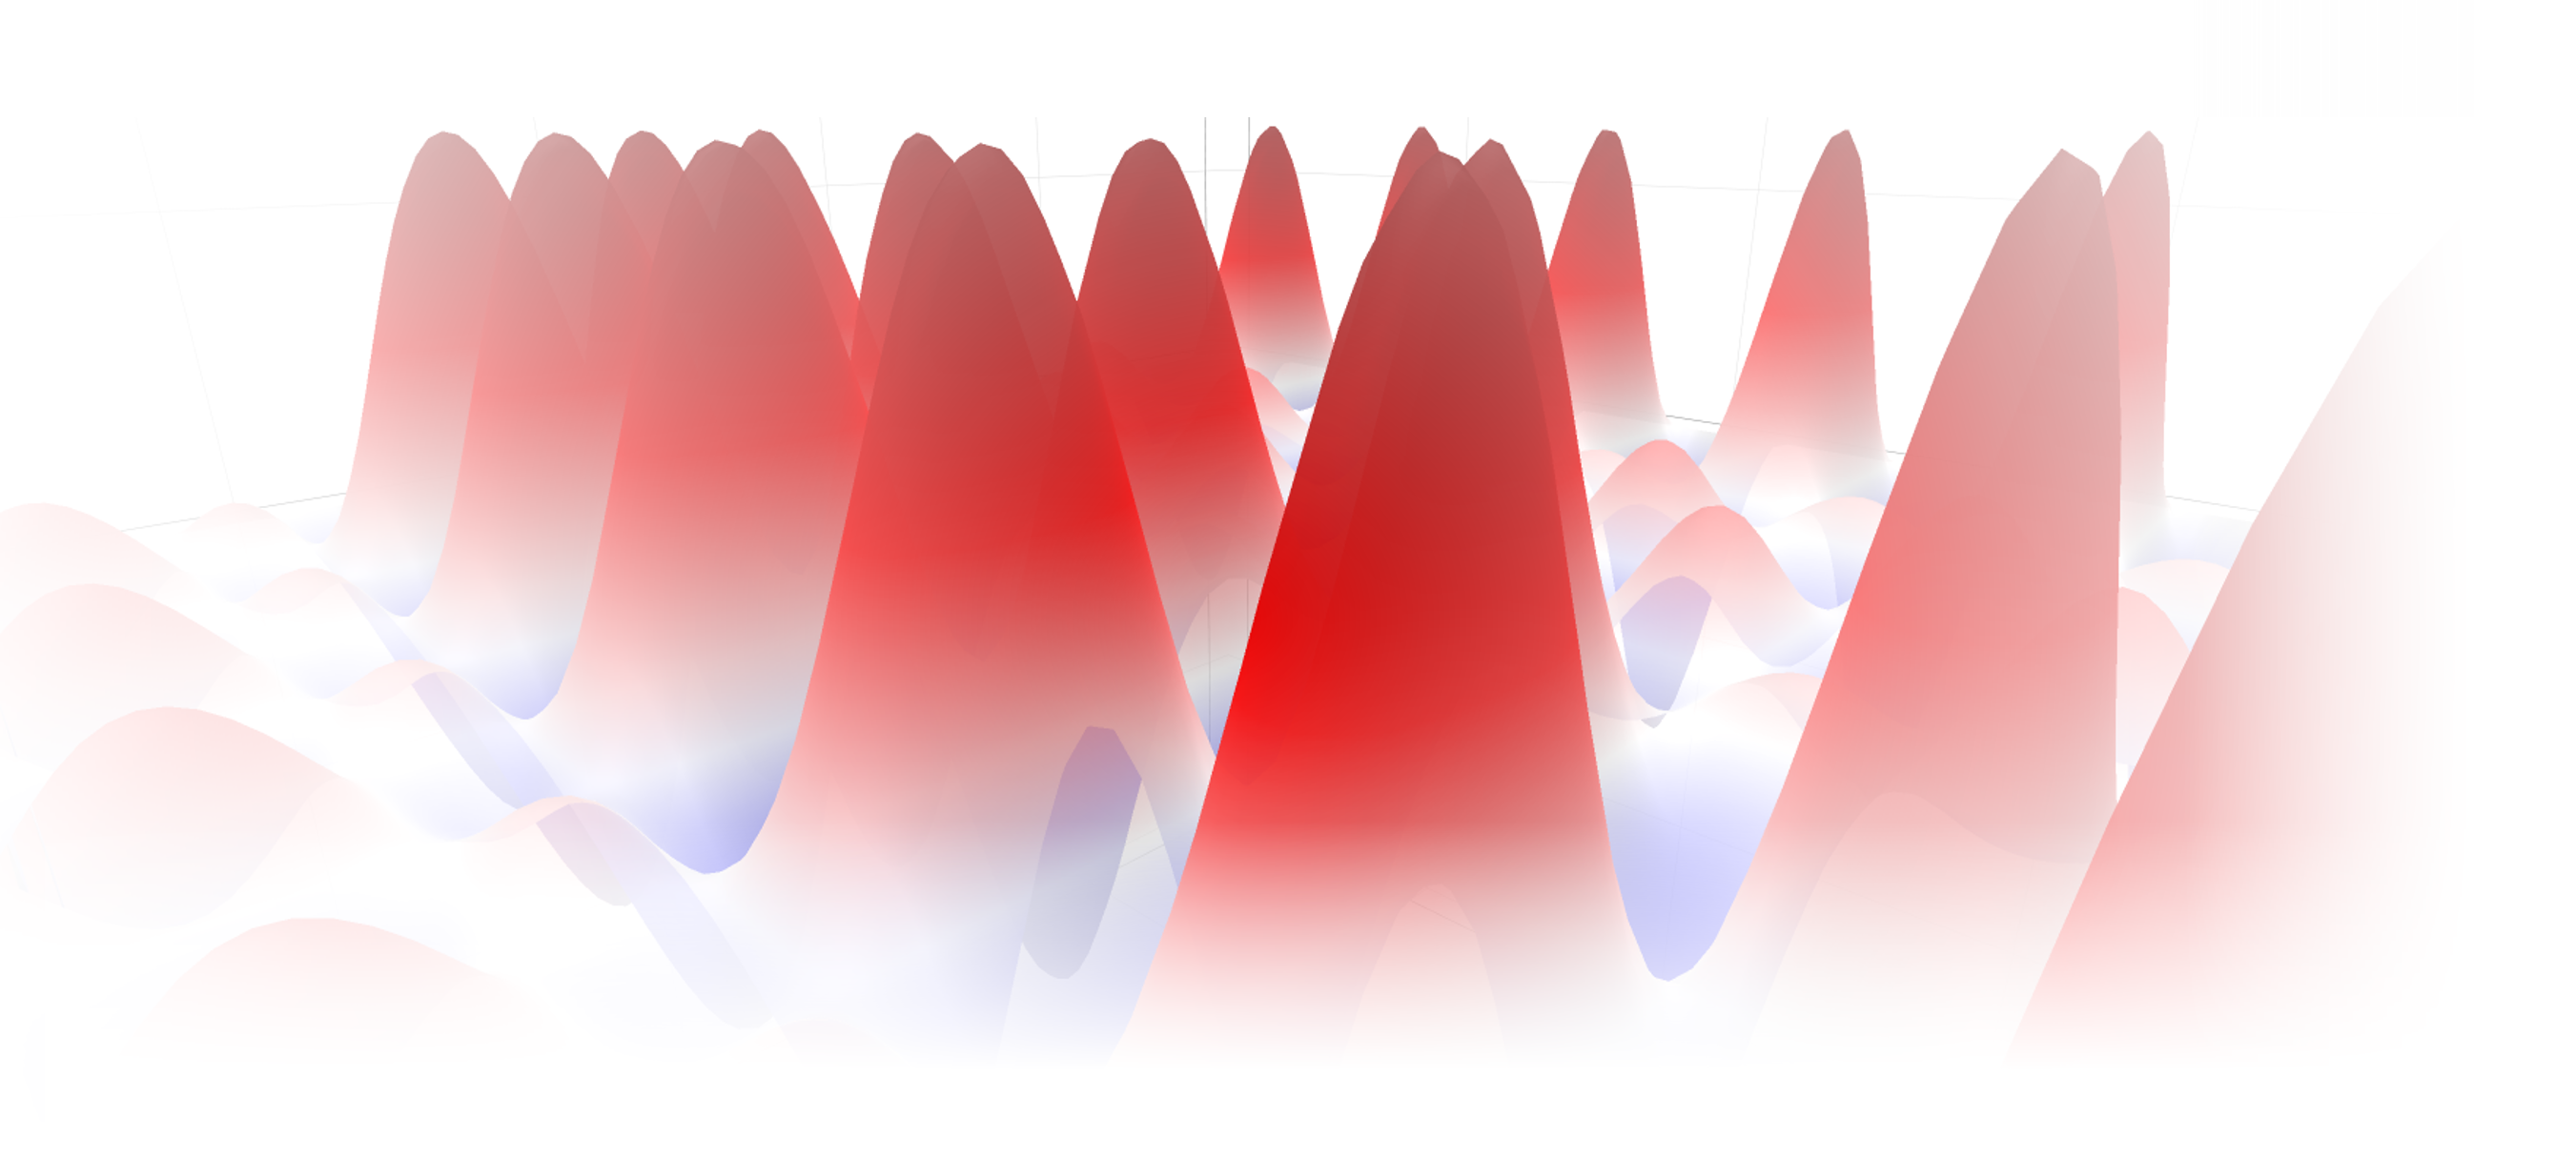
\includegraphics[width=1\textwidth, 
    trim={0cm 0 0 2.3cm}, clip]{cover_picture.png}
\end{center}

  \vfill\par
  \begin{flushright}
    \sffamily
    \@advisors\par
    \@department, ETH Z\"urich
  \end{flushright}
}

\checkandfixthelayout

\setlength{\droptitle}{-48pt}

\makeatother

% This defines how theorems should look. Best leave as is.
\theoremstyle{plain}
\setlength\theorempostskipamount{0pt}

%%% Local Variables:
%%% mode: latex
%%% TeX-master: "thesis"
%%% End:


%% Theorem environments.  You will have to adapt this for a German
%% thesis.
%% Theorem-like environments

%% This can be changed according to language. You can comment out the ones you
%% don't need.

\numberwithin{equation}{chapter}

%% German theorems
%\newtheorem{satz}{Satz}[chapter]
%\newtheorem{beispiel}[satz]{Beispiel}
%\newtheorem{bemerkung}[satz]{Bemerkung}
%\newtheorem{korrolar}[satz]{Korrolar}
%\newtheorem{definition}[satz]{Definition}
%\newtheorem{lemma}[satz]{Lemma}
%\newtheorem{proposition}[satz]{Proposition}

%% English variants
\newtheorem{theorem}{Theorem}[chapter]
\newtheorem{example}[theorem]{Example}
\newtheorem{remark}[theorem]{Remark}
\newtheorem{corollary}[theorem]{Corollary}
\newtheorem{definition}[theorem]{Definition}
\newtheorem{lemma}[theorem]{Lemma}
\newtheorem{proposition}[theorem]{Proposition}

%% Proof environment with a small square as a "qed" symbol
\theoremstyle{nonumberplain}
\theorembodyfont{\normalfont}
\theoremsymbol{\ensuremath{\square}}
\newtheorem{proof}{Proof}
%\newtheorem{beweis}{Beweis}


%% Helpful macros.
%% Custom commands
%% ===============

%% Special characters for number sets, e.g. real or complex numbers.
\newcommand{\C}{\mathbb{C}}
\newcommand{\K}{\mathbb{K}}
\newcommand{\N}{\mathbb{N}}
\newcommand{\Q}{\mathbb{Q}}
\newcommand{\R}{\mathbb{R}}
\newcommand{\Z}{\mathbb{Z}}
\newcommand{\X}{\mathbb{X}}

%% Fixed/scaling delimiter examples (see mathtools documentation)
\DeclarePairedDelimiter\abs{\lvert}{\rvert}
\DeclarePairedDelimiter\norm{\lVert}{\rVert}

%% Use the alternative epsilon per default and define the old one as \oldepsilon
\let\oldepsilon\epsilon
\renewcommand{\epsilon}{\ensuremath\varepsilon}

% physics stuff
% quantum states
\newcommand{\oo}{\ensuremath{\ket{11}}}
\newcommand{\zz}{\ensuremath{\ket{00}}}
\newcommand{\oz}{\ensuremath{\ket{10}}}
\newcommand{\zo}{\ensuremath{\ket{01}}}
\newcommand{\tz}{\ensuremath{\ket{20}}}
\newcommand{\zt}{\ensuremath{\ket{02}}}

\newcommand{\0}{\ensuremath{\ket{0}}}
\newcommand{\1}{\ensuremath{\ket{1}}}
\newcommand{\2}{\ensuremath{\ket{2}}}

\newcommand{\g}{\ensuremath{\ket{g}}}
\newcommand{\e}{\ensuremath{\ket{e}}}
\newcommand{\f}{\ensuremath{\ket{f}}}

% units
\newcommand{\degree}{\ensuremath{^\circ}}
% Math
% straight symbols
\renewcommand{\i}{\mathrm i}
\let\d\undefined 
\newcommand{\d}{\ensuremath{\,\mathrm d}}
\newcommand{\unit}[1]{\ensuremath{\,\mathrm{#1}}}
\newcommand{\sexp}[1]{\ensuremath{\mathrm e^{#1}}}
\newcommand{\us}{\ensuremath{\,\mu\textrm{s}}}

\newcommand{\transpose}[1]{\ensuremath{#1^\intercal}}

% quantum stuff
\newcommand{\costhamiltonian}{\ensuremath{\hat C}}
\newcommand{\ry}[1]{\ensuremath{Y(#1)}}
\newcommand{\rx}[1]{\ensuremath{X(#1)}}
\newcommand{\szsz}[2]{\ensuremath{\sigma_{#1}^z \sigma_{#2}^z}}
\renewcommand{\t}[1]{\ensuremath{T_{#1}}}

% qaoa stuff
\newcommand{\cost}{\ensuremath{C(\vec\gamma, \vec\beta)}}
\newcommand{\costh}{\ensuremath{\hat C}} % cost hamiltonian
\newcommand{\qaoa}[1]{\gls{qaoa}$_{#1}$}

\newcommand{\qaoaMeasuredState}{\ensuremath{|\vec{\gamma}, \vec{\beta}\rangle}}
\newcommand{\optimalstate}{\ensuremath{\ket{\psi_\mathrm{opt}}}}

\DeclareMathOperator*{\argmin}{arg\,min}
\DeclareMathOperator*{\argmax}{arg\,max}

% table stuff
\newcommand{\STAB}[1]{\begin{tabular}{@{}c@{}}#1\end{tabular}}
\newcommand{\HRule}{\rule{\linewidth}{0.5mm}}

%% Make document internal hyperlinks wherever possible. (TOC, references)
%% This MUST be loaded after varioref, which is loaded in 'extrapackages'
%% above.  We just load it last to be safe.
\usepackage[linkcolor=black,colorlinks=true,citecolor=black,filecolor=black, backref=page]{hyperref}
% configure back references
\renewcommand*{\backref}[1]{}
\renewcommand*{\backrefalt}[4]{{%
    \ifcase #1 Not cited.%
          \or Cited on page~#2.%
          \else Cited on pages #2.%
    \fi%
    }}


\makeglossaries

%% Document information
%% ====================

\title{Implemention of three-level readout and controlled arbitrary phase gates for quantum optimization algorithms with superconducting circuits}
\author{N. Lacroix}
\thesistype{Master Thesis}
\advisors{Advisors: Prof.\ Dr.\ A. Wallraff, Dr.\ C.K. Andersen}
\department{Department of Solid States Physics}
\date{January 14, 2020}

\begin{document}

\frontmatter

%% Title page is autogenerated from document information above.  DO
%% NOT CHANGE.
\begin{titlingpage}
  \calccentering{\unitlength}
  \begin{adjustwidth*}{\unitlength-24pt}{-\unitlength-24pt}
    \maketitle
  \end{adjustwidth*}
\end{titlingpage}

%% The abstract of your thesis.  Edit the file as needed.
\chapter{Abstract}
Large-scale, fault-tolerant quantum computing has the potential to impact numerous fields such as medical research, material science and information security. However, near-term quantum computers will only have a limited number of quantum bits and a limited quantum circuit size that can be executed reliably.

\Glspl{vqa} mitigate the consequences of these constraints by outsourcing part of the computation to classical computers and seeking approximate -- instead of exact -- solutions.  However, the gate sequence length that can be executed still remains limited by noise, in particular decoherence. Hence, most implementations so far are restricted to problem instances that can be solved with low depth circuits. Nevertheless, real-world applications involving a higher number of qubits will most likely require deeper circuits to approximate solutions accurately. 

In this thesis, we present and implement a two-qubit gate that takes advantage of the structure in the \gls{qaoa} to reduce the sequence length of the algorithm. Namely, we extend the standard \gls{cz} to a \gls{carb} by exploiting off-resonant interaction mechanisms and careful calibration of gate length, interaction strength and dynamic phases. Our implementation of the \gls{carb} achieves an average process fidelity of 97.7\%, which we measure with process tomography.

In addition, we demonstrate the advantage of \glspl{carb} on a 3-qubit \gls{qaoa} implementation solving an exact cover problem instance. We reduce the two-qubit gate-count by 50\% and the sequence length by a factor of 3 compared to a decomposed implementation with standard CZ gates. Consequently, we achieve a higher success probability with the direct implementation (0.84 versus 0.64) and foresee an increasing advantage for larger-scale problems because  the  number  of  layers  required  for a good approximate solution typically  scales with the number of  qubits in the problem.

% TODO:
% qaoa landscape symmetries
% outlook surface 7 experiment. + check qaoa plan

\glsresetall{}

%% TOC with the proper setup, do not change.
\cleartorecto
\tableofcontents
\cleartorecto
\listoffigures
\cleartorecto
\listoftables
\cleartorecto
\newacronym{carb}{C-ARB gate}{Controlled arbitrary angle phase gate}
\newacronym{cz}{CZ gate}{Controlled phase gate}
\newacronym{vqa}{VQA}{Variational quantum algorithm}
\newacronym{qaoa}{QAOA}{Quantum approximative optimization algorithm}
\newacronym{vqe}{VQE}{Variational quantum eigensolver}
\newacronym{cqed}{cQED}{Circuit quantum electrodynamics}
\newacronym{nisq}{NISQ}{Noisy intermediate scale quantum}
\newacronym{iir}{IIR}{Infinite Impulse Response}
\newacronym{fir}{FIR}{Finite Impulse Response}
\newacronym{qpt}{QPT}{Quantum process tomography}
\newacronym{pp}{pp.}{Percentage point}
\printglossary[type=\acronymtype] 

\mainmatter

%% Your real content!
% Some commands used in this file
\newcommand{\package}{\emph}

\chapter{Introduction}

This is version \verb-v1.4- of the template.

We assume that you found this template on our institute's website, so
we do not repeat everything stated there.  Consult the website again
for pointers to further reading about \LaTeX{}.  This chapter only
gives a brief overview of the files you are looking at.

\section{Features}
\label{sec:features}

The rest of this document shows off a few features of the template
files.  Look at the source code to see which macros we used!

The template is divided into \TeX{} files as follows:
\begin{enumerate}
\item \texttt{thesis.tex} is the main file.
\item \texttt{extrapackages.tex} holds extra package includes.
\item \texttt{layoutsetup.tex} defines the style used in this document.
\item \texttt{theoremsetup.tex} declares the theorem-like environments.
\item \texttt{macrosetup.tex} defines extra macros that you may find
  useful.
\item \texttt{introduction.tex} contains this text.
\item \texttt{sections.tex} is a quick demo of each sectioning level
  available.
\item \texttt{refs.bib} is an example bibliography file.  You can use
  Bib\TeX{} to quote references.  For example, read
  \cite{bringhurst1996ets} if you can get a hold of it.
\end{enumerate}


\subsection{Extra package includes}

The file \texttt{extrapackages.tex} lists some packages that usually
come in handy.  Simply have a look at the source code.  We have
added the following comments based on our experiences:
\begin{description}
\item[REC] This package is recommended.
\item[OPT] This package is optional.  It usually solves a specific
  problem in a clever way.
\item[ADV] This package is for the advanced user, but solves a problem
  frequent enough that we mention it. Consult the package's
  documentation.
\end{description}

As a small example, here is a reference to the Section \emph{Features}
typeset with the recommended \package{varioref} package:
\begin{quote}
  See Section~\vref{sec:features}.
\end{quote}


\subsection{Layout setup}

This defines the overall look of the document -- for example, it
changes the chapter and section heading appearance.  We consider this
a `do not touch' area.  Take a look at the excellent \emph{Memoir}
documentation before changing it.

In fact, take a look at the excellent \emph{Memoir} documentation,
full stop.


\subsection{Theorem setup}

This file defines a bunch of theorem-like environments.

\begin{theorem}
  An example theorem.
\end{theorem}

\begin{proof}
  Proof text goes here.
\end{proof}

Note that the q.e.d.\ symbol moves to the correct place automatically
if you end the proof with an \texttt{enumerate} or
\texttt{displaymath}.  You do not need to use \verb-\qedhere- as with
\package{amsthm}.

\begin{theorem}[Some Famous Guy]
  Another example theorem.
\end{theorem}

\begin{proof}
  This proof
  \begin{enumerate}
  \item ends in an enumerate.
  \end{enumerate}
\end{proof}

\begin{proposition}
  Note that all theorem-like environments are by default numbered on
  the same counter.
\end{proposition}

\begin{proof}
  This proof ends in a display like so:
  \begin{displaymath}
    f(x) = x^2.
  \end{displaymath}
\end{proof}


\subsection{Macro setup}

For now the macro setup only shows how to define some basic macros,
and how to use a neat feature of the \package{mathtools} package:
\begin{displaymath}
  \abs{a}, \quad \abs*{\frac{a}{b}}, \quad \abs[\big]{\frac{a}{b}}.
\end{displaymath}

% \chapter{Writing scientific texts in English}

This chapter was originally a separate document written by Reto
Spöhel.  It is reprinted here so that the template can serve as a
quick guide to thesis writing, and to provide some more example
material to give you a feeling for good typesetting.

% We're going to need an extra theorem-like environment for this
% chapter
\theoremstyle{plain}
\theoremsymbol{}
\newtheorem{Rule}[theorem]{Rule}

\section{Basic writing rules}

The following rules need little further explanation; they are best
understood by looking at the example in the booklet by Knuth et al.,
§2--§3.

\begin{Rule}
  Write texts, not chains of formulas.
\end{Rule}

More specifically, write full sentences that are logically
interconnected by phrases like `Therefore', `However', `On the other
hand', etc.\ where appropriate.

\begin{Rule}
  Displayed formulas should be embedded in your text and punctuated
  with it.
\end{Rule}

In other words, your writing should not be divided into `text parts'
and `formula parts'; instead the formulas should be tied together by
your prose such that there is a natural flow to your writing.

\section{Being nice to the reader}

Try to write your text in such a way that a reader enjoys reading
it. That's of course a lofty goal, but nevertheless one you should
aspire to!

\begin{Rule}
  Be nice to the reader.
\end{Rule}

Give some intuition or easy example for definitions and theorems which
might be hard to digest. Remind the reader of notations you introduced
many pages ago -- chances are he has forgotten them. Illustrate your
writing with diagrams and pictures where this helps the reader. Etc.

\begin{Rule}
  Organize your writing.
\end{Rule}

Think carefully about how you subdivide your thesis into chapters,
sections, and possibly subsections.  Give overviews at the beginning
of your thesis and of each chapter, so the reader knows what to
expect. In proofs, outline the main ideas before going into technical
details. Give the reader the opportunity to `catch up with you' by
summing up your findings periodically.

\emph{Useful phrases:} `So far we have shown that \ldots', `It remains
to show that \ldots', `Recall that we want to prove inequality (7), as
this will allow us to deduce that \ldots', `Thus we can conclude that
\ldots. Next, we would like to find out whether \ldots', etc.

\begin{Rule}
  Don't say the same thing twice without telling the reader that you
  are saying it twice.
\end{Rule}

Repetition of key ideas is important and helpful. However, if you
present the same idea, definition or observation twice (in the same or
different words) without telling the reader, he will be looking for
something new where there is nothing new.

\emph{Useful phrases:} `Recall that [we have seen in Chapter 5 that]
\ldots', `As argued before / in the proof of Lemma 3, \ldots', `As
mentioned in the introduction, \ldots', `In other words, \ldots', etc.

\begin{Rule}
  Don't make statements that you will justify later without telling
  the reader that you will justify them later.
\end{Rule}

This rule also applies when the justification is coming right in the
next sentence!  The reasoning should be clear: if you violate it, the
reader will lose valuable time trying to figure out on his own what
you were going to explain to him anyway.

\emph{Useful phrases:} `Next we argue that \ldots', `As we shall see,
\ldots', `We will see in the next section that \ldots, etc.


\section{A few important grammar rules}

\begin{Rule}
  \label{rule:no-comma-before-that}
  There is (almost) \emph{never} a comma before `that'.
\end{Rule}

It's really that simple. Examples:
\begin{quote}
  We assume that \ldots\\
  \emph{Wir nehmen an, dass \ldots}

  It follows that \ldots\\
  \emph{Daraus folgt, dass \ldots}

  `thrice' is a word that is seldom used.\\
  \emph{`thrice' ist ein Wort, das selten verwendet wird.}
\end{quote}
Exceptions to this rule are rare and usually pretty obvious. For
example, you may end up with a comma before `that' because `i.e.' is
spelled out as `that is':
\begin{quote}
  For \(p(n)=\log n/n\) we have \ldots{} However, if we choose \(p\) a
  little bit higher, that is \(p(n)=(1+\varepsilon)\log n/n\) for some
  \(\varepsilon>0\), we obtain that\ldots
\end{quote}
Or you may get a comma before `that' because there is some additional
information inserted in the middle of your sentence:
\begin{quote}
  Thus we found a number, namely \(n_0\), that satisfies equation (13).
\end{quote}
If the additional information is left out, the sentence has no comma:
\begin{quote}
  Thus we found a number that satisfies equation (13).
\end{quote}
(For `that' as a relative pronoun, see also
Rules~\ref{rule:non-defining-has-comma}
and~\ref{rule:defining-without-comma} below.)

\begin{Rule}
  There is usually no comma before `if'.
\end{Rule}

Example:
\begin{quote}
  A graph is not \(3\)-colorable if it contains a \(4\)-clique.\\
  \emph{Ein Graph ist nicht \(3\)-färbbar, wenn er eine \(4\)-Clique
    enthält.}
\end{quote}
However, if the `if' clause comes first, it is usually separated from
the main clause by a comma:
\begin{quote}
  If a graph contains a \(4\)-clique, it is not \(3\)-colorable .\\
  \emph{Wenn ein Graph eine \(4\)-Clique enthält, ist er nicht
    \(3\)-färbbar.}
\end{quote}

There are more exceptions to these rules than to
Rule~\ref{rule:no-comma-before-that}, which is why we are not
discussing them here. Just keep in mind: don't put a comma before `if'
without good reason.

\begin{Rule}
  \label{rule:non-defining-has-comma}
  Non-defining relative clauses have commas.
\end{Rule}
\begin{Rule}
  \label{rule:defining-without-comma}
  Defining relative clauses have no commas.
\end{Rule}

In English, it is very important to distinguish between two types of
relative clauses: defining and non-defining ones. This is a
distinction you absolutely need to understand to write scientific
texts, because mistakes in this area actually distort the meaning of
your text!

It's probably easier to explain first what a \emph{non-defining}
relative clause is. A non-defining relative clauses simply gives
additional information \emph{that could also be left out} (or given in
a separate sentence). For example, the sentence
\begin{quote}
  The \textsc{WeirdSort} algorithm, which was found by the famous
  mathematician John Doe, is theoretically best possible but difficult
  to implement in practice.
\end{quote}
would be fully understandable if the relative clause were left out
completely. It could also be rephrased as two separate sentences:
\begin{quote}
  The \textsc{WeirdSort} algorithm is theoretically best possible but
  difficult to implement in practice. [By the way,] \textsc{WeirdSort}
  was found by the famous mathematician John Doe.
\end{quote}
This is what a non-defining relative clause is. \emph{Non-defining
  relative clauses are always written with commas.} As a corollary we
obtain that you cannot use `that' in non-defining relative clauses
(see Rule~\ref{rule:no-comma-before-that}!). It would be wrong to
write
\begin{quote}
  \st{The \textsc{WeirdSort} algorithm, that was found by the famous
    mathematician John Doe, is theoretically best possible but
    difficult to implement in practice.}
\end{quote}
A special case that warrants its own example is when `which' is
referring to the entire preceding sentence:
\begin{quote}
  Thus inequality (7) is true, which implies that the Riemann
  hypothesis holds.
\end{quote}
As before, this is a non-defining relative sentence (it could be left
out) and therefore needs a comma.

So let's discuss \emph{defining} relative clauses next. A defining
relative clause tells the reader \emph{which specific item the main
  clause is talking about}. Leaving it out either changes the meaning
of the sentence or renders it incomprehensible altogether.  Consider
the following example:

\begin{quote}
  The \textsc{WeirdSort} algorithm is difficult to implement in
  practice. In contrast, the algorithm that we suggest is very simple.
\end{quote}

Here the relative clause `that we suggest' cannot be left out -- the
remaining sentence would make no sense since the reader would not know
which algorithm it is talking about. This is what a defining relative
clause is. \textit{Defining relative clauses are never written with
  commas.} Usually, you can use both `that' and `which' in defining
relative clauses, although in many cases `that' sounds better.

As a final example, consider the following sentence:
\begin{quote}
  For the elements in \(\mathcal{B}\) which satisfy property (A), we
  know that equation (37) holds.
\end{quote}
This sentence does not make a statement about all elements in
\(\mathcal{B}\), only about those satisfying property (A). The relative
clause is \emph{defining}. (Thus we could also use `that' in place of
`which'.)

In contrast, if we add a comma the sentence reads
\begin{quote}
  For the elements in \(\mathcal{B}\), which satisfy property (A), we
  know that equation (37) holds.
\end{quote}

Now the relative clause is \emph{non-defining} -- it just mentions in
passing that all elements in \(\mathcal{B}\) satisfy property (A). The
main clause states that equation (37) holds for \emph{all} elements in
\(\mathcal{B}\). See the difference?


\section[Things you (usually) don't say in English]%
{Things you (usually) don't say in English -- and what to say
  instead}
\label{sec:list}

Table~\ref{tab:things-you-dont-say} lists some common mistakes and
alternatives.  The entries should not be taken as gospel -- they don't
necessarily mean that a given word or formulation is wrong under all
circumstances (obviously, this depends a lot on the context). However,
in nine out of ten instances the suggested alternative is the better
word to use.

\begin{table}
  \centering
  \caption{Things you (usually) don't say}
  \label{tab:things-you-dont-say}
  \begin{tabular}{lll}
    \toprule
    \st{It holds (that) \dots} & We have \dots & \emph{Es gilt \dots}\\
    \multicolumn{3}{l}{\quad\footnotesize(`Equation (5) holds.' is fine, though.)}\\
    \st{$x$ fulfills property $\mathcal{P}$.}& \(x\) satisfies property \(\mathcal{P}\). & \emph{\(x\) erfüllt Eigenschaft \(\mathcal{P}\).} \\
    \st{in average} & on average & \emph{im Durchschnitt}\\
    \st{estimation} & estimate   & \emph{Abschätzung}\\
    \st{composed number} & composite number & \emph{zusammengesetzte Zahl}\\
    \st{with the help of} & using & \emph{mit Hilfe von}\\
    \st{surely} & clearly & \emph{sicher, bestimmt}\\
    \st{monotonously increasing} & monotonically incr. & \emph{monoton steigend}\\
    \multicolumn{3}{l}{\quad\footnotesize(Actually, in most cases `increasing' is just fine.)}\\
    \bottomrule
  \end{tabular}
\end{table}

%%% Local Variables:
%%% mode: latex
%%% TeX-master: "thesis"
%%% End:

% \chapter{Typography}


\section{Punctuation}

\begin{Rule}
  Use opening (`) and closing (') quotation marks correctly.
\end{Rule}

In \LaTeX, the closing quotation mark is typed like a normal
apostrophe, while the opening quotation mark is typed using the French
\emph{accent grave} on your keyboard (the \emph{accent grave} is the
one going down, as in \emph{frère}).

Note that any punctuation that \emph{semantically} follows quoted
speech goes inside the quotes in American English, but outside in
Britain.  Also, Americans use double quotes first.  Oppose
\begin{quote}
  ``Using `lasers,' we punch a hole in \ldots\ the Ozone Layer,''
  Dr.\ Evil said.
\end{quote}
to
\begin{quote}
  `Using ``lasers'', we punch a hole in \ldots\ the Ozone Layer',
  Dr.\ Evil said.
\end{quote}

\begin{Rule}
  Use hyphens (-), en-dashes (--) and em-dashes (---) correctly.
\end{Rule}

A hyphen is only used in words like `well-known', `$3$-colorable'
etc., or to separate words that continue in the next line (which is
known as hyphenation).  It is entered as a single ASCII hyphen
character (\texttt{-}).

To denote ranges of numbers, chapters, etc., use an en-dash (entered
as two ASCII hyphens \texttt{--}) with no spaces on either side.  For
example, using Equations (1)--(3), we see\ldots

As the equivalent of the German \emph{Gedankenstrich}, use an en-dash
with spaces on both sides -- in the title of Section \ref{sec:list},
it would be wrong to use a hyphen instead of the dash. (Some English
authors use the even longer emdash (---) instead, which is typed as
three subsequent hyphens in \LaTeX. This emdash is used without spaces
around it---like so.)


\section{Spacing}

\begin{Rule}
  \label{rule:no-manual-spacing}
  Do not add spacing manually.
\end{Rule}

You should never use the commands \lstinline-\\- (except within
tabulars and arrays), \lstinline[showspaces=true]-\ - (except to
prevent a sentence-ending space after Dr.\ and such),
\lstinline-\vspace-, \lstinline-\hspace-, etc.  The choices programmed
into \LaTeX{} and this style should cover almost all cases.  Doing it
manually quickly leads to inconsistent spacing, which looks terrible.
Note that this list of commands is by no means conclusive.

\begin{Rule}
  Judiciously insert spacing in maths where it helps.
\end{Rule}

This directly contradicts Rule~\ref{rule:no-manual-spacing}, but in
some cases \TeX{} fails to correctly decide how much spacing is
required.  For example, consider
\begin{displaymath}
  f(a,b) = f(a+b, a-b).
\end{displaymath}
In such cases, inserting a thin math space \lstinline-\,- greatly
increases readability:
\begin{displaymath}
  f(a,b) = f(a+b,\, a-b).
\end{displaymath}

Along similar lines, there are variations of some symbols with
different spacing.  For example, Lagrange's Theorem states that
\(\abs{G}=[G:H]\abs{H}\), but the proof uses a bijection \(f\colon
aH\to bH\).  (Note how the first colon is symmetrically spaced, but
the second is not.)

\begin{Rule}
  Learn when to use \lstinline[showspaces=true]-\ - and
  \lstinline-\@-.
\end{Rule}

Unless you use `french spacing', the space at the end of a sentence is
slightly larger than the normal interword space.

The rule used by \TeX{} is that any space following a period,
exclamation mark or question mark is sentence-ending, except for
periods preceded by an upper-case letter.  Inserting \lstinline-\-
before a space turns it into an interword space, and inserting
\lstinline-\@- before a period makes it sentence-ending.  This means
you should write
\begin{lstlisting}
Prof.\ Dr.\ A. Steger is a member of CADMO\@.
If you want to write a thesis with her, you
should use this template.
\end{lstlisting}
which turns into
\begin{quote}
  Prof.\ Dr.\ A. Steger is a member of CADMO\@.  If you want to write
  a thesis with her, you should use this template.
\end{quote}
The effect becomes more dramatic in lines that are stretched slightly
during justification:
\begin{quote}
  \parbox{\linewidth}{\hbox to \linewidth{%
      Prof.\ Dr.\ A. Steger is a member of CADMO\@.  If you}}
\end{quote}

\begin{Rule}
  Place a non-breaking space (\lstinline-~-) right before references.
\end{Rule}

This is actually a slight simplification of the real rule, which
should invoke common sense.  Place non-breaking spaces where a line
break would look `funny' because it occurs right in the middle of a
construction, especially between a reference type (Chapter) and its
number.


\section{Choice of `fonts'}

Professional typography distinguishes many font attributes, such as
family, size, shape, and weight.  The choice for sectional divisions
and layout elements has been made, but you will still occasionally
want to switch to something else to get the reader's attention.  The
most important rule is very simple.

\begin{Rule}
  When emphasising a short bit of text, use \lstinline-\emph-.
\end{Rule}

In particular, \emph{never} use bold text (\lstinline-\textbf-).
Italics (or Roman type if used within italics) avoids distracting the
eye with the huge blobs of ink in the middle of the text that bold
text so quickly introduces.

Occasionally you will need more notation, for example, a consistent
typeface used to identify algorithms.

\begin{Rule}
  Vary one attribute at a time.
\end{Rule}

For example, for \textsc{WeirdSort} we only changed the shape to small
caps.  Changing two attributes, say, to bold small caps would be
excessive (\LaTeX{} does not even have this particular variation).
The same holds for mathematical notation: the reader can easily
distinguish \(g_n\), \(G(x)\), \(\mathcal{G}\) and \(\mathsf{G}\).

\begin{Rule}
  Never underline or uppercase.
\end{Rule}

No exceptions to this one, unless you are writing your thesis on a
typewriter.  Manually.  Uphill both ways.  In a blizzard.


\section{Displayed equations}

\begin{Rule}
  Insert paragraph breaks \emph{after} displays only where they
  belong.  Never insert paragraph breaks \emph{before} displays.
\end{Rule}

\LaTeX{} translates sequences of more than one linebreak (i.e., what
looks like an empty line in the source code) into a paragraph break in
almost all contexts.  This also happens before and after displays,
where extra spacing is inserted to give a visual indication of the
structure.  Adding a blank line in these places may look nice in the
sources, but compare the resulting display

\begin{displaymath}
  a = b
\end{displaymath}

to the following:
\begin{displaymath}
  a = b
\end{displaymath}
The first display is surrounded by blank lines, but the second is not.
It is bad style to start a paragraph with a display (you should always
tell the reader what the display means first), so the rule follows.

\begin{Rule}
  Never use \lstinline-eqnarray-.
\end{Rule}

It is at the root of most ill-spaced multiline displays.  The
\package{amsmath} package provides better alternatives, such as the
\lstinline-align- family
\begin{align*}
  f(x) &= \sin x, \\
  g(x) &= \cos x,
\end{align*}
and \lstinline-multline- which copes with excessively long equations:
\begin{multline*}
  \def\P{\mathrm P}
  \P\bigl[X_{t_0} \in (z_0, z_0+dz_0],\ldots, X_{t_n}\in(z_n,z_n+dz_n]\bigr]
  \\= \nu(dz_0) K_{t_1}(z_0,dz_1) K_{t_2-t_1}(z_1,dz_2)\cdots
  K_{t_n-t_{n-1}}(z_{n-1},dz_n).
\end{multline*}


\section{Floats}

By default this style provides floating environments for tables and
figures.  The general structure should be as follows:
\begin{lstlisting}
\begin{figure}
  \centering
  % content goes here
  \caption{A short caption}
  \label{some-short-label}
\end{figure}
\end{lstlisting}
Note that the label must follow the caption, otherwise the label will
refer to the surrounding section instead.  Also note that figures
should be captioned at the bottom, and tables at the top.

The whole point of floats is that they, well, \emph{float} to a place
where they fit without interrupting the text body.  This is a frequent
source of confusion and changes; please leave it as is.

\begin{Rule}
  Do not restrict float movement to only `here'
  \textnormal{(\lstinline-h-)}.
\end{Rule}

If you are still tempted, you should avoid the float altogether and
just show the figure or table inline, similar to a displayed equation.

%%% Local Variables:
%%% mode: latex
%%% TeX-master: "thesis"
%%% End:

\chapter{The Transmon and Circuit Quantum Electrodynamics}
\chapter{High fidelity qutrit single shot readout} \label{ch:qutrit_readout}
\chapter{Calibrating and Characterizing Controlled Arbitrary Phase Gates} \label{ch:carb}
\glsreset{carb}
This chapter details the concepts, calibration and characterization of \glspl{carb}. We start by explaining how this gate family can be seen as an extension of standard conditional phase gate (\glspl{cz}). Next, we demonstrate the implementation of a \gls{carb}, allowing us to reach continuous conditional phase in the range $[0, 2\pi[$. We describe the calibration procedure of the gate on qubit 2 and 3 of our quantum processor presented in Appendix~\ref{app:setup}. Next, perform quantum process tomography and evaluate the process fidelity as a function of conditional phase. By exploiting the 3-level readout discussed in Appendix~\ref{ch:qutrit_readout}, we then characterize conditional- and dynamic phase errors and leakage. We compare these phase errors and leakage values to the ones obtained with a \gls{cz} implemented on the same qubits.

\section{Theoretical description} \label{sec:c_arb_theory}
In this section, we derive the unitary evolution of the \gls{carb} and explain the physical mechanisms behind its implementation. The goal is to obtain a unitary operator $U_{\textrm{C-ARB}}$ in a two-qubit subspace which adds a controllable phase $\phi$ to the \oo{} state, 
\begin{equation} \label{eq:carb_unitary}
    U_{\textrm{C-ARB}}=
    \begin{pmatrix}
{1} & {0} & {0} & {0} \\
{0} & {1} & {0} & {0} \\
{0} & {0} & {1} & {0} \\
{0} & {0} & {0} & {e^{-\i \phi}}
\end{pmatrix}
\end{equation}

We obtain such unitary by exploiting the same effect as for the \gls{cz}, namely the collection of geometric phase on the \oo{} state due to the interaction of the \oo{} level and the non-computational \tz{} level~\cite{Strauch2003QuantumQubits, DiCarlo2009DemonstrationProcessor}. As pictured in Fig.~\ref{fig:carb_theory}(a),  the \oo{} and \tz{} levels hybridize strongly when they are brought close to resonance. In this regime, we can approximate their interaction as a two-level system where the ground (excited) state is the \oo{} (\tz{}) state. The system is characterized by the Hamiltonian
\begin{equation}
    \hat H/\hbar= \omega_{\ket{11}} \oo{} \bra{11} + \omega_{\ket{20}} \tz{} \bra{20} + J( \oo{}\bra{20}+ \tz{}\bra{11})
\end{equation}
where  $\omega_{\ket{11}}$ ($\omega_{\ket{20}}$) is the frequency of the energy level \oo{} (\tz{}), and $J$ is the fixed coupling strength between the two levels which is a chip design parameter fixed during fabrication. The first and second term in the Hamiltonian correspond to the energy in the \oo{} and \tz{} level respectively. The third term represents the coupling energy between the two levels in which the excitation is transferred from one level to the other and vice-versa. 

The same Hamiltonian can conveniently be written in matrix form with basis vectors \oo{} and \tz{},
\begin{equation}
\hat{H}/\hbar=
\begin{pmatrix}
\omega_{\oo} & J \\
J & \omega_{\tz}
\end{pmatrix}
\end{equation}
We shift the zero energy to $\omega_{\oo}$  and define the frequency detuning between the two levels $\Delta = \omega_{\tz}- \omega_{\oo}$ such that $\hat H$ becomes
\begin{equation}
\hat{H}/\hbar=
\begin{pmatrix}
0 & J \\
J & \Delta
\end{pmatrix}
\end{equation}

From Schr\"odinger's equation, it follows that the time evolution of an arbitrary state $\ket{\psi}$ in the \oo-\tz{} subspace is given by $|\psi(t)\rangle = U(t)\ket{\psi}$ where $U(t) = \sexp{-\i \hat H/\hbar t}$ is the unitary evolution of the Hamiltonian. Specifically, the unitary $U(t)$ is defined as,
\begin{equation}
\begin{split}
    &U(t) = \\
& \begin{pmatrix}
 \sexp{-\frac{1}{2} \i t \Delta } \left(\cos \left(\frac{1}{2} t \Tilde{J} \right)+\frac{\i \Delta  \sin \left(\frac{1}{2} t \Tilde{J}\right)}{\Tilde{J}}\right) & -\frac{2 \i e^{-\frac{1}{2} \i t
   \Delta } J \sin \left(\frac{1}{2} t \Tilde{J}\right)}{\Tilde{J}} \\
 -\frac{2 \i e^{-\frac{1}{2} \i t \Delta } J \sin \left(\frac{1}{2} t \Tilde{J}\right)}{\Tilde{J}} & \sexp{-\frac{1}{2} \i t \Delta }
   \left(\cos \left(\frac{1}{2} t \Tilde{J}\right)-\frac{\i \Delta 
   \sin \left(\frac{1}{2} t \Tilde{J}\right)}{\Tilde{J}}\right) \\
\end{pmatrix}
\end{split}
\end{equation}
where we have defined for clarity $\Tilde{J} := \sqrt{4J^2+\Delta^2}$ which we call the \textit{effective exchange coupling}.

When starting with an excitation in the \oo{} state (the ground-state of this two-level subsystem), the \oo{} population oscillates coherently as the excitation is swapped back and forth between the \oo{} and the \tz{} state,
\begin{equation}
P_{\oo{}}(t) = \mathrm{Tr}\left(U(t)\ket{11}\bra{11}U^\dag(t)\right) = \frac{\Delta ^2+2 J^2 (\cos \left(t \sqrt{4J^2+\Delta^2}\right)+1)}{4J^2+\Delta^2}
\end{equation}
with an oscillation period of $2\pi/\Tilde{J}$. 

The population as function of frequency detuning $\Delta$ and interaction time $t$ results in a Chevron pattern shown in Fig.~\ref{fig:carb_theory}(b). For the operating point of the \gls{cz}, $\Delta = 0$, the population is given by $P_{\oo{}} = \frac{1}{2} + \frac{1}{2}\cos{2Jt}$. This corresponds to a complete population exchange between the \oo{} and the \tz{} state and with an oscillation period of $\pi/J$. By contrast, $\Delta \neq 0$ results in a partial population exchange between the \oo{} and the \tz{} state. The oscillation period is also reduced due to the detuning $\Delta$ in the denominator. 

\begin{figure}
    \centering
    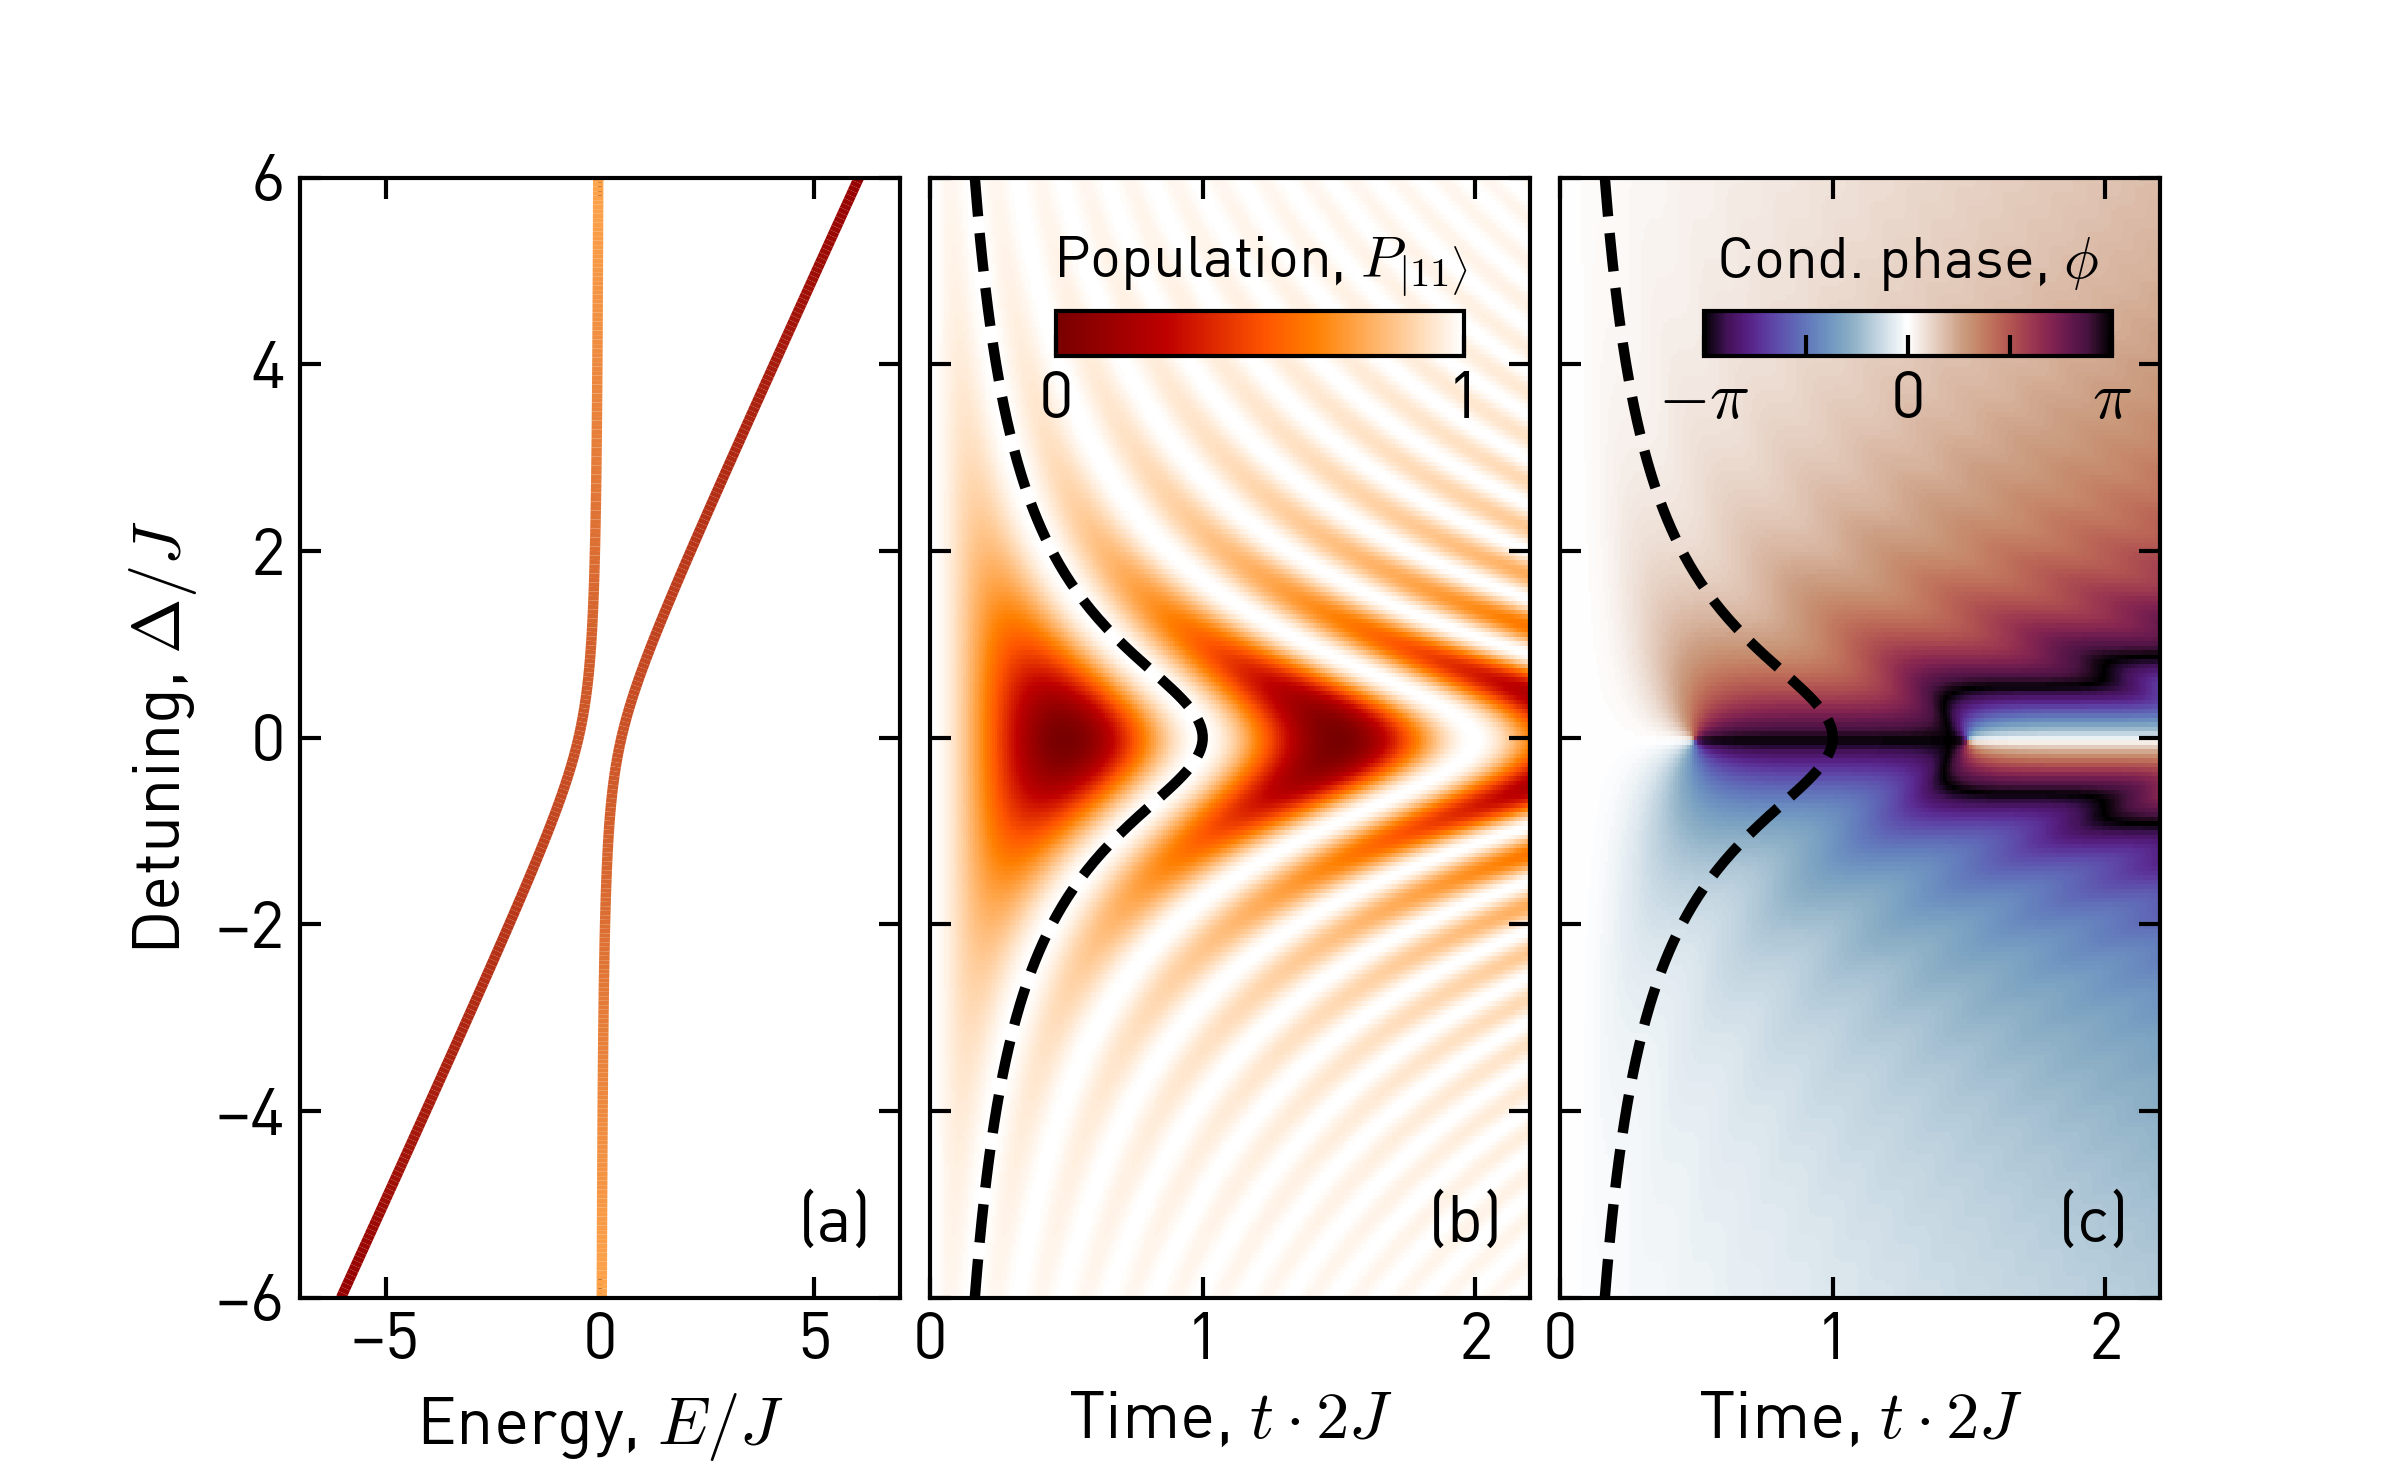
\includegraphics[width=1\textwidth]{chapters/carb_gate/figs/ch4_carb_theory_c3_20200312_095516.png}
    \caption{Simulation of the \gls{carb} as a generalization of the \gls{cz}. (a) Avoided crossing between the \oo{} (brown) and the \tz{} (orange) energy levels as function of detuning. (b) Population of the \oo{} state as function of frequency detuning $\Delta$ and interaction time $t$ (in units of $J$) visualizing the coherent population exchange due to hybridization. The dashed line corresponds to the frequency detunings and gate lengths resulting in the first maximum in population recovery in the computational subspace. (c) Conditional phase acquired on the \oo{} state resulting from the interaction of the two levels. We reach all conditional phases between 0 and $2\pi$ by sweeping the detuning and adapting the time accordingly to ensure population recovery (dashed line). }
    \label{fig:carb_theory}
\end{figure}

The gate length must be an integer multiple of the oscillation period to ensure a unitary operation within the computational subspace (i.e.\ full population recovery). In Fig.~\ref{fig:carb_theory}(b), we highlight (dashed line) the first oscillation period which corresponds to the shortest possible gate length as a function of the frequency detuning,
\begin{equation} \label{eq:carb_t_gate}
    t_{\textrm{C-ARB}} = \frac{2\pi}{\sqrt{4J^2+\Delta^2}}
\end{equation}

In  Fig.~\ref{fig:carb_theory}(c),  we illustrate the acquired conditional phase, $\phi$, as a function of detuning and gate length. For the gate lengths $t_{\textrm{C-ARB}}$, the corresponding phase on the \oo{} state acquired by the closed loop state evolution is
 \begin{equation} \label{eq:ch4_acquired_cond_phase}
     \phi = \mathrm{Arg}\Big(\bra{11}U(t_{\textrm{C-ARB}})\oo\Big) =  \pi \cdot \left( 1 + \frac { \Delta } { \sqrt { \Delta ^ { 2 } + 4 J ^ { 2 } } } \right)
 \end{equation}
which spans the interval $[0, 2\pi[$ for a sufficiently large detuning sweep, see dashed line in Fig.~\ref{fig:carb_theory}(c). As expected, a zero detuning yields a conditional phase of $\pi$ and therefore corresponds to the standard \gls{cz}.

In practice, we achieve these timed interactions with flux pulses\footnote{In fact, we apply a \textit{voltage} pulse at the output of the \gls{awg} and the latter creates a current in the flux line which results in magnetic flux through the SQUID loop} which shift the transition frequency of the individual qubits. For a gate in the off-state, we ensure $|\Delta|\gg J$ such that the acquired conditional phase is small. Ideally, the acquired phase should be zero but in practice it is not due to the residual $ZZ$-coupling between the \oo{} and the \tz{} state. To turn on the gate, we apply a square flux pulse with amplitude $a$ and length $l$ to one of the qubits via its flux line. The pulse shifts the \oo{} state non-adiabatically close to the \tz{} state. 

As mentioned in Section~\ref{sec:intro_building_qc}, the flux affects the Josephson energy~\cite[Eq.~2.18]{KochCharge-insensitiveBox}, 
\begin{equation}\
    E_J(a) = E _ { J , \max } \sqrt { \cos ^ { 2 } \left( \frac{\pi}{\Phi_0} \frac { \partial \Phi } { \partial V } a \right) + d ^ { 2 } \sin ^ { 2 } \left( \frac{\pi}{\Phi_0}\frac { \partial \Phi} { \partial V } a \right) }
\end{equation}
where $d$ is the asymmetry between the junctions in the SQUID loop of the transmon, $ \partial \Phi /\partial V $ is the flux sensitivity (voltage to flux conversion parameter), $\Phi_0 = h/2e$ is the superconducting flux quantum and $E _ { J , \max }$ is the maximal junction energy. 

In turn, the Josephson energy shifts the qubit transition frequency as defined by Eq.~\eqref{eq:qubit_frequency} such that
\begin{equation} \label{eq:carb_theory_freq01}
    \omega_{|01\rangle}(a) \simeq \sqrt{8  E _ { J , \max } \sqrt { \cos ^ { 2 } \left( \frac{\pi}{\Phi_0}\frac { \partial \Phi } {  \partial V } a \right) + d ^ { 2 } \sin ^ { 2 } \left( \frac{\pi}{\Phi_0}\frac { \partial \Phi} { \partial V } a \right)} E_{C}}-E_{C} 
\end{equation}
where we approximate $|E_c|$ to be equal to the anharmonicity $|\alpha_2|$ of the fluxed transmon~\cite[Eq. 2.12]{KochCharge-insensitiveBox}. 
The frequency detuning, $\Delta$, as function of the flux pulse amplitude is then simply
 \begin{equation}\label{eq:carb_detuning}
\begin{aligned} 
\Delta(a) & = \omega _ { | 20 \rangle } - \omega _ { | 11 \rangle } \\ 
& = 2 \omega _ { | 10 \rangle } - \alpha _ { 1 } - \left( \omega _ { | 10 \rangle } + \omega _ { | 01 \rangle }(a) \right) \\ 
& = \omega _ { | 10 \rangle } - \alpha _ { 1 } - \omega _ { | 01 \rangle }(a) 
\end{aligned}
\end{equation}
where $\alpha_1$ is the anharmonicity of the  transmon which is not fluxed.

It follows that varying the amplitude of the flux pulse indeed controls the frequency detuning between the \oo{} and the \tz{} state, which in turn controls the collected phase on the \oo{} state. To ensure full population recovery in the computational subspace, the length of the flux pulse must be $t_{\textrm{C-ARB}}$ which can be related back to the amplitude of the flux pulse by combining Eq.~\eqref{eq:carb_t_gate}, \eqref{eq:carb_theory_freq01} and \eqref{eq:carb_detuning},
\begin{equation} \label{eq:carb_t_gate_from_ampl}
\begin{split}
    &t_{\textrm{C-ARB}}(a)\simeq\\
    &   \frac{2\pi}{\sqrt{4J^2+\left(\omega _ { | 10 \rangle } - \alpha _ { 1 } - \sqrt{8  E _ { J , \max } \sqrt { \cos ^ { 2 } \left( \frac{\pi}{\Phi_0}\frac { \partial \Phi } {  \partial V } a \right) + d ^ { 2 } \sin ^ { 2 } \left( \frac{\pi}{\Phi_0}\frac { \partial \Phi} { \partial V } a \right)} \alpha_2} - \alpha_2 \right)^2}}
\end{split}
\end{equation}
In Section~\ref{sec:carb_calibration}, we fit Eq.~\eqref{eq:carb_t_gate_from_ampl} to experimental data to estimate $J$, $ \partial \Phi/ \partial V $ and $d$ and thereby also the expected conditional phase using Eq.~\eqref{eq:ch4_acquired_cond_phase}.

In addition to the conditional phase, the flux pulse also results in a dynamic phase $\phi_D$ on the fluxed qubit,  because it takes the qubit out of its rotating frame~\cite{DiCarlo2009DemonstrationProcessor},
\begin{equation} \label{eq:carb_dyn_phase}
    \phi_D = \int_0^l{(\omega(t)-\omega_{\textrm{park}})\d t}
\end{equation}
where $\omega(t)$ and $\omega_{\textrm{park}}$ denote the instantaneous qubit frequency during the pulse and the frequency at parking position\footnote{The parking position refers to the frequency of the qubit when the gate is off. We typically choose it to be where the derivative of the frequency with respect to flux is 0 to minimize the charge noise, a point we call the "sweet spot"~\cite{Vion2003QuantumProcessing}}, respectively. We compensate for this single-qubit phase shift with a virtual $Z$ gate after the \gls{carb}.

While the \gls{cz} is composed of from a single detuning and gate length, the \gls{carb} requires a careful interpolation of distinct detunings and corresponding gate lengths to span all possible conditional phases with high \oo{} population recovery. In addition, since the qubit frequency excursion depends on $\Delta$, dynamic phases have to be calibrated for all possible detuning/gate-length pairs. We detail the calibration procedure of these three continuous parameters in the next section.

\section{Calibration} \label{sec:carb_calibration}
This section describes the calibration procedure of a \gls{carb} using a square flux pulse on qubit 2 and 3 of the device presented in Appendix~\ref{app:setup}. To account for the finite rise-time and ensure a stable voltage at the output of the \gls{awg}, we filter the square pulse with a 1\unit{ns} Gaussian kernel. The calibration of the \gls{carb} consists of three measurements, illustrated in Fig.~\ref{fig:ch4_calibration_carb}.

First, we calibrate the pulse lengths to ensure maximum population recovery. We prepare the \oo{} state and perform a two-dimensional sweep of the flux pulse amplitude and length. For each amplitude and length, we measure the \1{} population of qubit 2 after the flux pulse using 3-level readout, yielding the Chevron pattern shown in Fig.~\ref{fig:ch4_calibration_carb}(a). Brighter areas correspond to high
level population of qubit 2, indicating the population is fully swapped back from the \2{} level into the computational subspace. To find the pulse lengths corresponding to the first period of the population exchange, we fit the \1{} population oscillation to a cosine for each pulse amplitude of the two-dimensional sweep. We then retrieve the pulse length corresponding to the first maximum of the population recovery.

We fit the pulse lengths corresponding the maximum population recovery to Eq.~\eqref{eq:carb_t_gate_from_ampl} to extract the flux sensitivity $\frac { \partial \Phi} { \partial V }$, the asymmetry between the junctions in the SQUID loop $d$  and the coupling strength $J$ between the \oo{} and \tz{} states. The fit is shown as a dashed line in Fig.~\ref{fig:ch4_calibration_carb}(a). We obtain a flux sensitivity of $\frac { \partial \Phi} { \partial V } / \Phi_0 = 0.34 \pm 0.01 \unit{\frac{1}{V}}$, an asymmetry of $0.7884 \pm 0.0003$ and a coupling of $J/2\pi =  4.72 \pm 0.05 \unit{MHz}$, all of which are consistent with previous characterization of this device~\cite{Andersen2019, Andersen2019a}.

Next, we measure the conditional phase as function of flux pulse amplitudes (see Fig.~\ref{fig:ch4_calibration_carb}(b)) while adapting the pulse length to maximize population recovery (see Fig.~\ref{fig:ch4_calibration_carb}(a), black circles). If necessary, pulse length is interpolated linearly between the calibration points of the pulse length calibration. The colored flux pulses shown in the pulse scheme in Fig.~\ref{fig:ch4_calibration_carb}(e) correspond to the diamond-shaped data points of respective color in ~\ref{fig:ch4_calibration_carb}(b). Using the parameter values obtained from the fit in Fig.~\ref{fig:ch4_calibration_carb}(a), we compute the expected conditional phase from  Eq.~\eqref{eq:ch4_acquired_cond_phase} and plot it in dashed line in Fig.~\ref{fig:ch4_calibration_carb}(b). The measured conditional phase saturates at a value of different than 0 due the phase acquired via the a residual $ZZ$-coupling of $\alpha_{ZZ} = 400\unit{kHz}$ over the period the pulse length and buffers (25ns) that separates the two $R_x^{\pi/2}$-pulses. 

Finally, we measure the dynamic phase the fluxed qubit acquires during its frequency excursion (see Fig.~\ref{fig:ch4_calibration_carb}(c)) with the pulse scheme presented in Fig.~\ref{fig:ch4_calibration_carb}(f)). With the approximation that its frequency is constant over the entire pulse at the value given by Eq.~\eqref{eq:carb_theory_freq01}, we compute the expected dynamic phase from Eq.~\eqref{eq:carb_dyn_phase} and show it with a dashed line. This measurement requires a high number of calibration points, as the dynamic phase grows rapidly as a function of detuning yet can only be measured in the $[0, 2\pi[$ interval (a minimum of 3 points per $[0, 2\pi[$ interval are required to ensure correct unwrapping). In Fig.~\ref{fig:ch4_calibration_carb}(c), only one out of three points is shown for clarity. 
\begin{figure}[H]
    \centering
    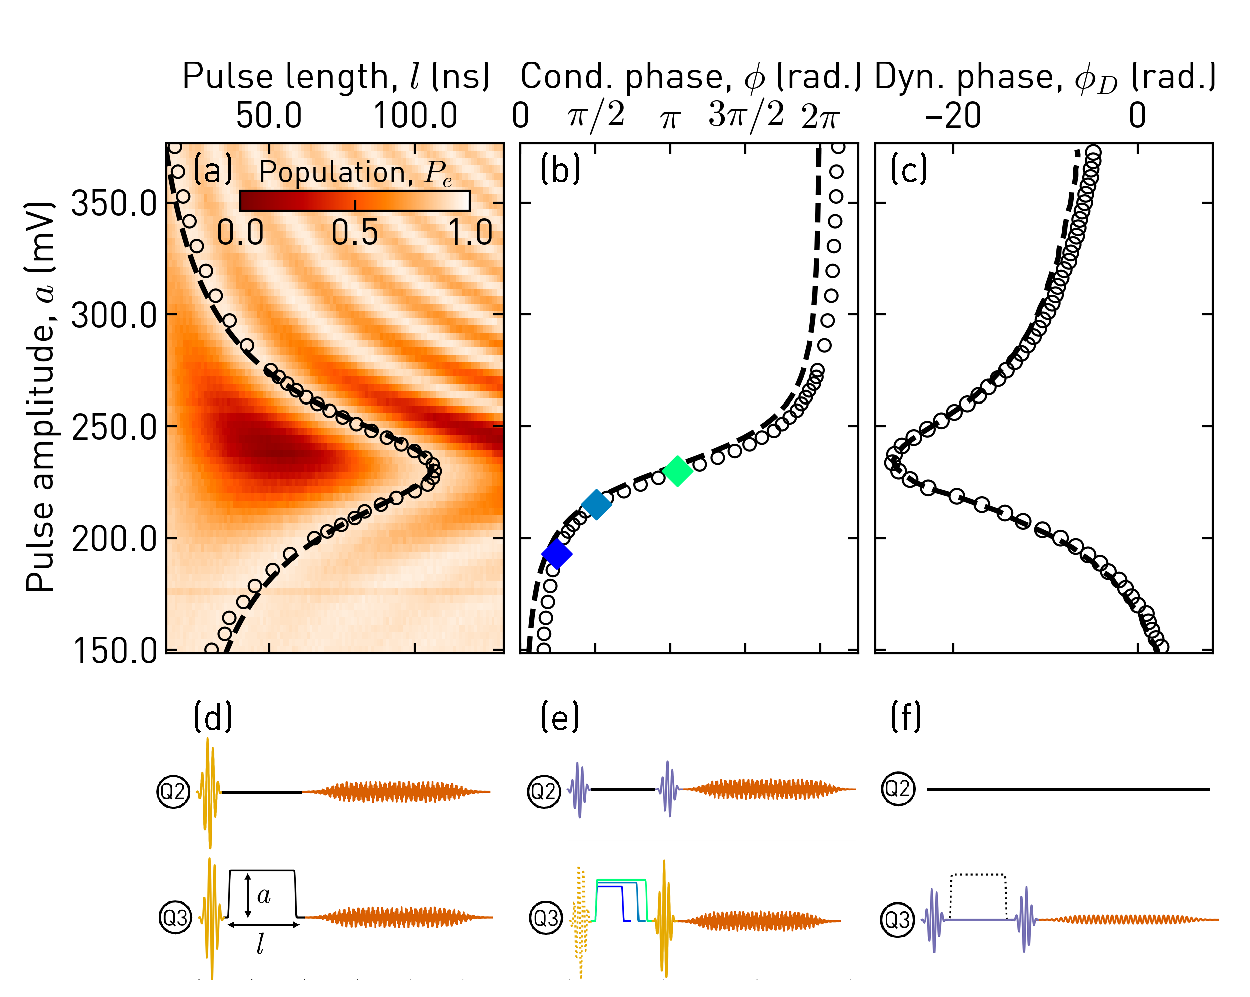
\includegraphics[width=\textwidth]{chapters/carb_gate/figs/ch4_carb_calibration_20200406_215519.pdf}
    \caption{Three calibration measurements (a, b, c) of a \gls{carb} and their corresponding pulse schemes (d, e, f).  (a) Qubit 2 \e{} level population as function of the flux pulse amplitude and length. The inset details the pulse scheme: the \oo{} state is prepared, the flux pluse (black) is  applied to qubit 3, the two qubits are read out with a multiplexed readout pulse. The scattered points correspond to the amplitudes and lengths used to calibrate the conditional phase (see b). The dashed line corresponds to the fit to the theoretical model. (b) Conditional phase as function of flux pulse amplitude. The amplitude sampling is not uniform to account for the non-linearity of the conditional phase. The dashed line indicates the phase predicted of the model (see main text for details).  (c) Unwrapped dynamic phase of qubit 3 as function of pulse amplitude. Only one out of three data point is shown for clarity.  The dashed line corresponds to the dynamic phase predicted by theory (see main text for details). (d) Pulse scheme corresponding to the two-dimensional parameter sweep shown in (a). The \oo{} state is prepared with two single-qubit $R_x^\pi$ (yellow), followed by the flux pulse (black) of amplitude $a$ and length $l$, and finally a readout pulse (orange). (e) Pulse scheme to measure conditional phase (see b). The phase is measured on qubit 2 with a Ramsey experiment (two $R_x^{\pi/2}$ pulses (purple)), while qubit 3 is fluxed once with and once without preceding single-qubit $R_x^{\pi}$ (dashed yellow). The difference between the two measurements yields the conditional phase. The different flux pulse colors result in the conditional phases indicated with diamonds of corresponding color in (b). (f) The dynamic phase is measured by comparing the phase of the qubit via a Ramsey experiment with and without flux pulse (dashed black).}
    \label{fig:ch4_calibration_carb}
\end{figure}

Due to flux cross-talk between the flux lines, the qubit staying at its parking position also acquires a non-zero dynamic phase. However, the latter is not calibrated, as flux cross-talk between the flux line of qubit 1 (3) and qubit 2 is smaller than 2\% (3\%) for the two two-qubit gates considered in this report~\cite{Andersen2018SampleB4QP3}.

The calibration time of the \gls{carb} on qubits 2 and 3 amounts to approximately 2 hours and 45 minutes i.e.\ about 5 to 8 times slower than a full calibration of a \gls{cz}. The high-resolution, two-dimensional amplitude/gate length sweep last for 1 hour, whilst for the conditional phase measurement (45 calibration points) requires 15 minutes, and the dynamic phase, 1 hour and 30 minutes. The following actions would reduce the calibration time:
\begin{itemize}
    \item[--] Use the active reset scheme discussed in Section~\ref{sec:active_reset}. This scheme allows an increase of the repetition rate by a factor of 5-10 leading to a total measurement time of 20-40 minutes.
    \item[--] Use a non-linear amplitude sampling for the dynamic phase based on the theoretical model. Namely, have an adaptable spacing between amplitudes at which the dynamic phase is calibrated based on whether the model predicts a large or small increase in dynamic phase. This would reduce the number of measurement point for the dynamic phase calibration by a factor of $\sim2$, compared to a dense linear pulse amplitude spacing.
    \item[--] Rewrite the dynamic phase measurement such that all waveforms are uploaded on the AWGs at once, instead of one at the time. This would reduce communication overhead.
\end{itemize}
Implementing these changes could in principle reduce the calibration time to under 20min per gate. Parallel tune up of two-qubit gates has the potential to decrease the calibration time of the device even further. 

In this section, we demonstrated the ability to calibrate a \gls{carb}. The next section details the characterization of the gate.

\begin{comment}
In addition to the pulse calibration, we use  \gls{iir} and \gls{fir} filters to predistort the pulses. compensate for the charge accumulation on the bias-tee and the frequency-dependent response of the flux line, we additionally pre-distort the pulse according to the procedure detailed in ~\cite{Butscher2018ShapingFiltering}
For the calibration of the \gls{iir} and \gls{fir} filters, which . The filters predistort the flux pulse to achieve the desired pulse shape at the quantum device.
\end{comment}

\section{Characterization} 
Randomized benchmarking -- the most common method to characterize two-qubit gates -- cannot be performed on the \gls{carb} because it is not part of the Clifford group~\cite{Magesan2011ScalableProcesses, Magesan2012CharacterizingBenchmarking}. Hence, we use another common method called quantum process tomography to characterize the \gls{carb}. Next, we perform a fine target phase sweep and characterize conditional and dynamic phase errors as well as leakage out of the computational subspace. Finally, we compare the performance of the \gls{carb} to the \gls{cz} and assess their  stability over a time (up to 15 hours after calibration).

\subsection{Quantum process tomography}
\Gls{qpt} is a method providing full description of a quantum process~\cite{Chuang1997PrescriptionBox, Poyatos1997CompleteGate}. In brief, it consists of preparing an ensemble of input states $\{\rho_1^\mathrm{in}, ..., \rho_k^\mathrm{in}\}$ spanning the Hilbert space of interest, passing them through the quantum process $\mathcal{E}$ and finally identifying the resultant states  $\{\rho_1^\mathrm{out}, ..., \rho_k^\mathrm{out}\}$ using quantum state tomography~\cite{Reed2013EntanglementQubits}. The output states are then
\begin{equation}
    \rho_k^{\mathrm{out}} = \mathcal{E}(\rho_k^\mathrm{in}) = \sum_{m n} \chi_{m n} P_n \rho_k^\mathrm{in} P_m^\dag
\end{equation}
 where $\chi$ is the process matrix and $P$ is the Pauli operator basis for 2 qubits: $P_n \in \{I, X, -\i Y, Z\}^{\otimes 2}$~\cite{HeinsooDigitalQubits}. The inversion of the above equation yields the desired process matrix $\chi$, which describes how the process affects an arbitrary input density matrix. 
 
The process fidelity $\mathcal{F}$ quantifies the closeness between the measured process matrix $\chi_\mathrm{exp}$ and the target matrix $\chi_\mathrm{targ}$~\cite{Schumacher1996SendingChannels}: 
 \begin{equation}
     \mathcal{F} = \mathrm{Tr}(\chi_\mathrm{exp} \chi_\mathrm{targ})
 \end{equation}
This metric quantifies how well the measured gate would act on half of a fully entangled system and if that action is identical to the target operation.
In the presence of leakage, the tomographic reconstruction of the computational subspace is not a trace-preserving map~\cite{Wood2018QuantificationErrors}. Therefore, we use the 3-level readout scheme discussed in Appendix~\ref{ch:qutrit_readout} to detect and exclude leakage events from the tomography measurement. We characterize leakage occuring during the gate separately in Section~\ref{sec:carb_characterization_phase_errors_leakage}. 
Readout noise can also lead to non-physical\footnote{A physical density matrix is positive semidefinite, Hermitian and trace preserving.} density matrix reconstructions. We use a maximum likelihood algorithm to find physical density matrices which are most likely to have been measured under the assumption of Gaussian noise~\cite{BaurRealizingQubits}. 
Finally, we correct for readout errors by multiplying the measured probabilities with the inverse of the readout probability matrix (see Section \ref{sec:qutrit_readout_correction} and Supplementary Material~\cite[suppl.~mat.]{Bialczak2010QuantumQubits}).

We perform \gls{qpt} for various target conditional phases of the \gls{carb}. Two resulting process matrices, $\chi^\pi$ and $\chi^{7\pi/4}$,  for target phases of $\pi$ and $7\pi/4$ respectively, are shown in Fig.~\ref{fig:carb_characterization_chi_matrices}. The black frame represents the target process matrices while the filled bars correspond to the reconstructed process matrices. We observe a good  agreement between them. In the chosen operator basis, a process matrix which can be described by a real unitary operator will also be real~\cite{Nielsen2000QuantumInformation}. This is the case for $\chi^\pi$, which is described by the real diagonal \gls{cz} unitary (see Eq.~\eqref{eq:carb_unitary} with $\phi = \pi$). By contrast, $\chi^{7\pi/4}$ is not described by a real unitary operator and therefore contains an imaginary part. On the diagonal of the real part, the same terms appear as in $\chi^{\pi}$, but with a different relative contribution. In particular, the $II$ contribution is higher, as adding a phase of $7\pi/4$ (nearly $2\pi$) on the \oo{} state is closer to an identity operation than adding a phase of $\pi$.

\begin{figure}[ht]
    \centering
    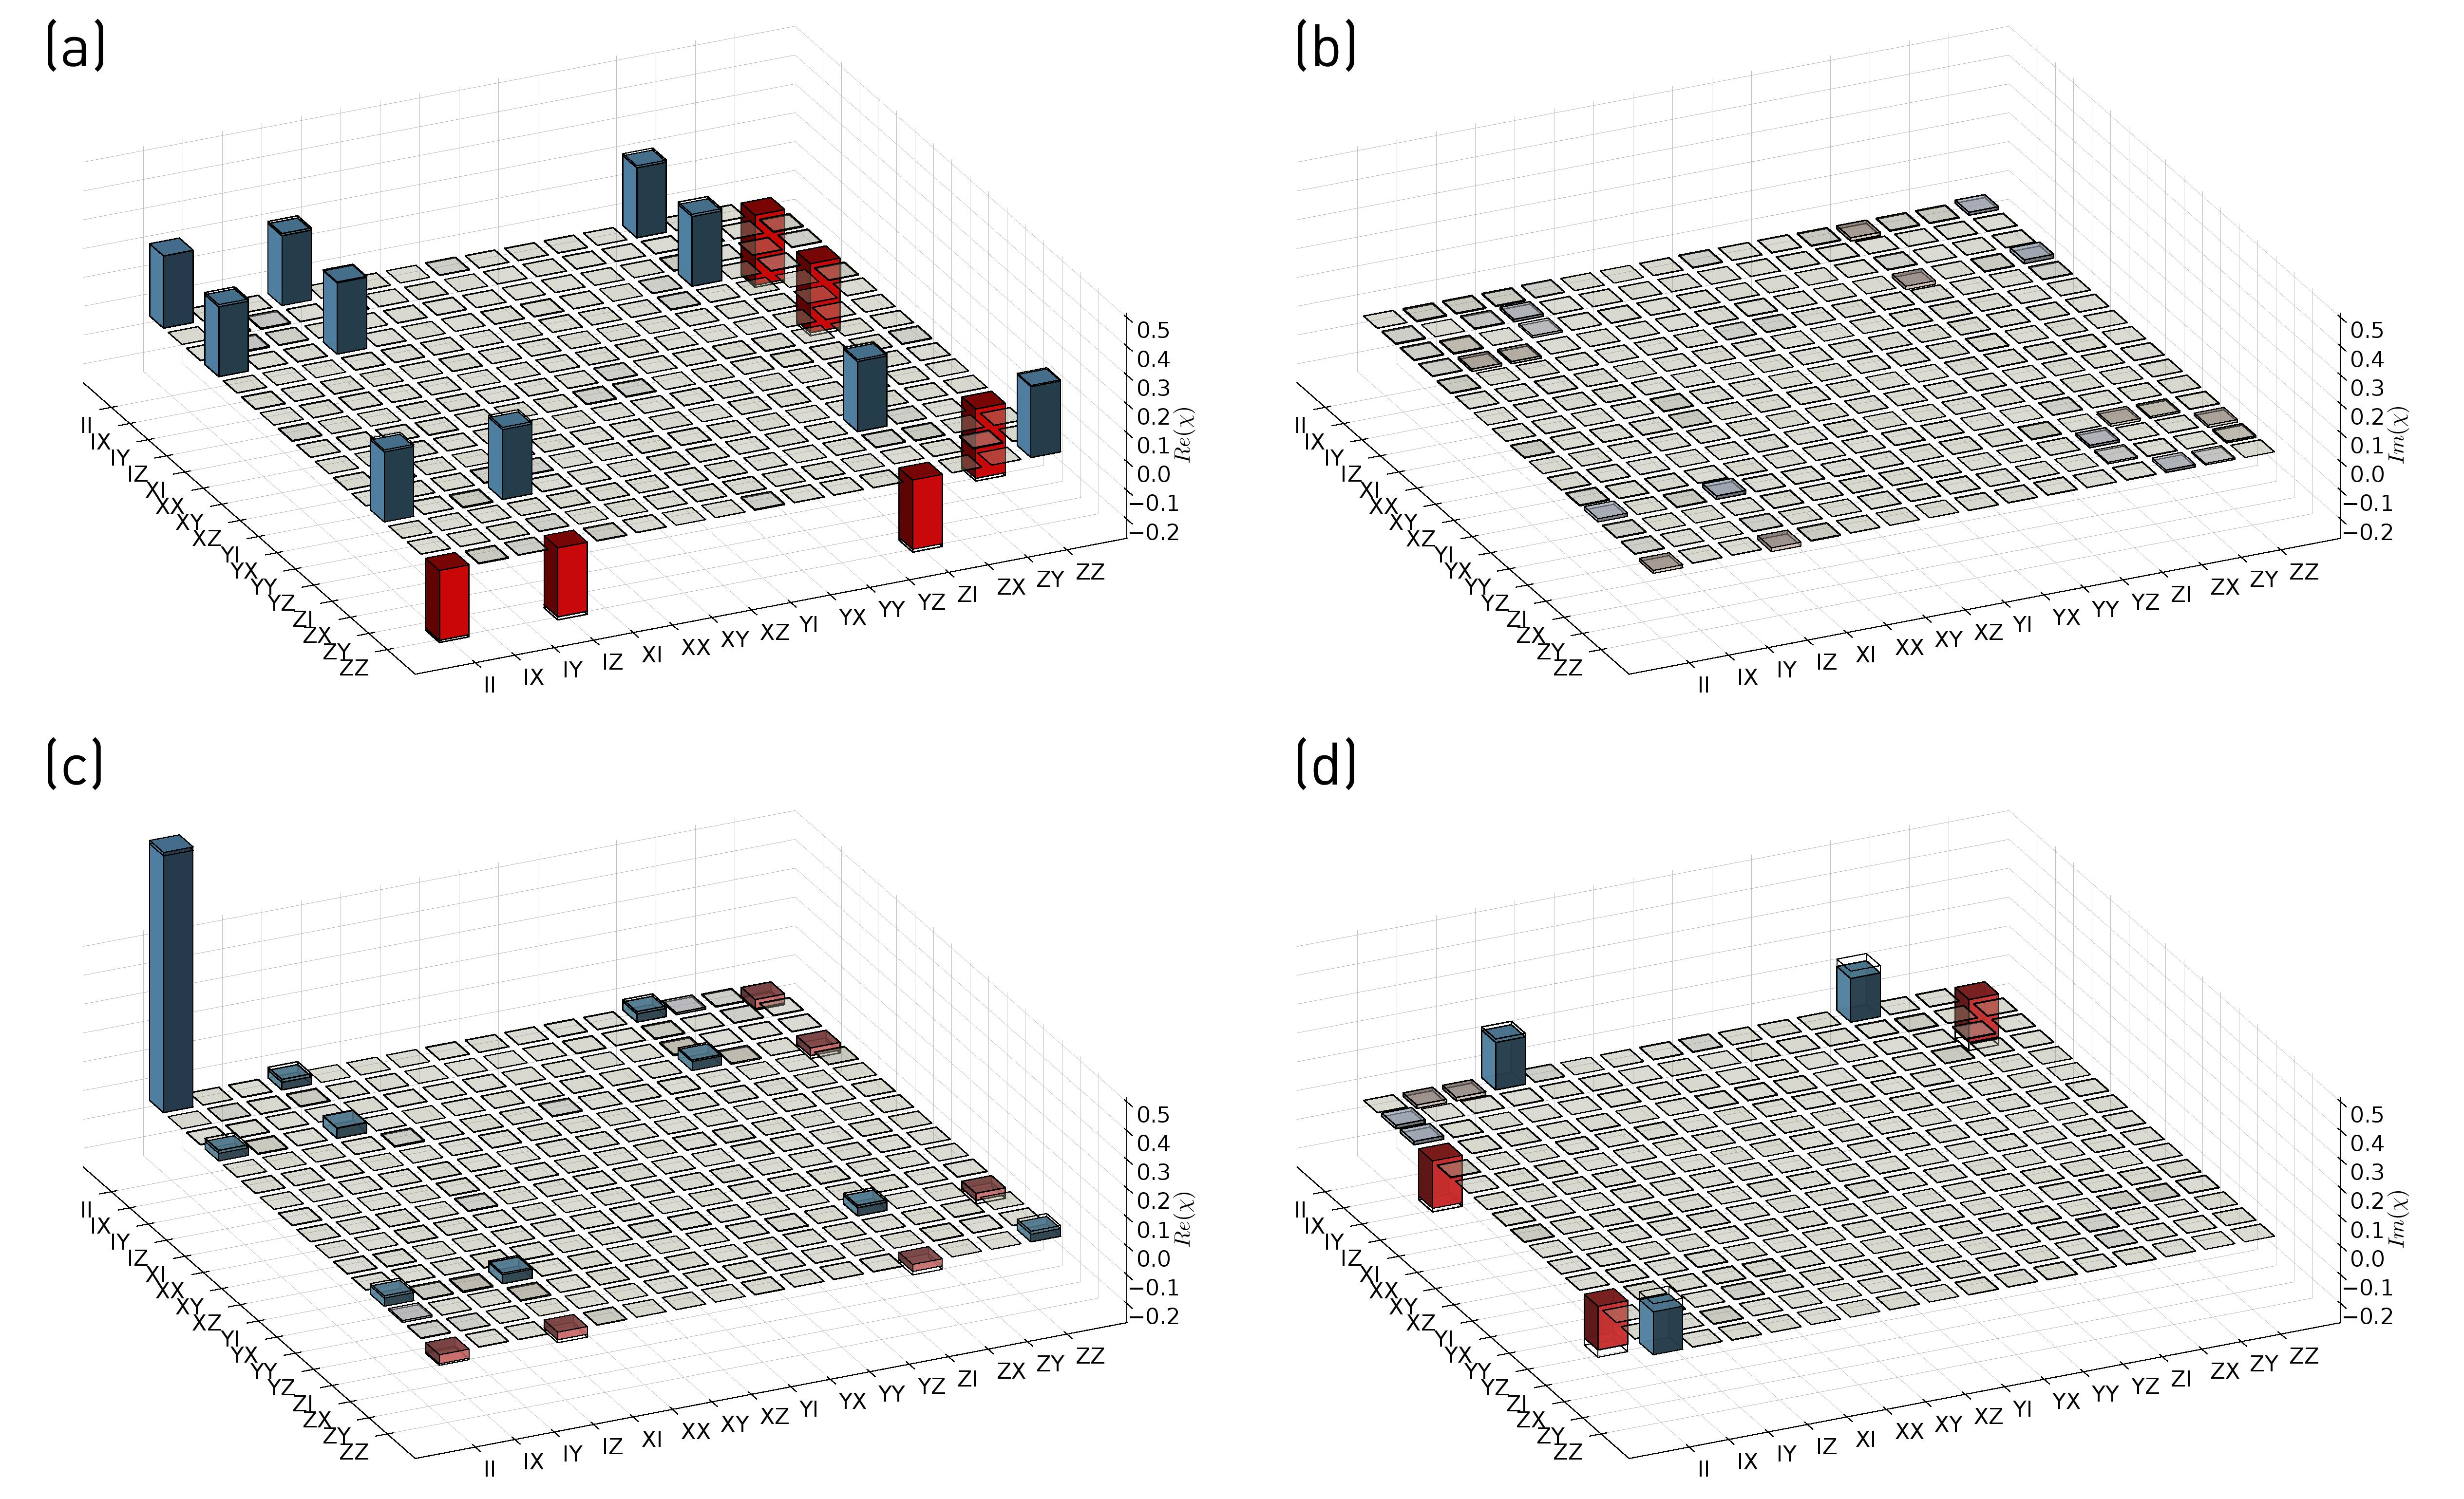
\includegraphics[width=\textwidth]{chapters/carb_gate/figs/process_tomography_chi_mtx.jpg}
    \caption{Real (a, c) and imaginary (b, d) elements of the process matrices $\chi^\pi$ and $\chi^{7\pi/4}$ respectively. The black wire frame corresponds to the target process matrix, while the blue (positive values) and red (negative values) filled bars correspond to the recontructed process matrix from measurements. The process fidelity for the phase  $\pi$ ($7\pi/4$) is 97.3\% (98.3\%).   }
    \label{fig:carb_characterization_chi_matrices}
\end{figure}

In Fig.~\ref{fig:carb_characterization_process_fidelity}, we show the process fidelity for 7 phase angles of the \gls{carb}. The maximum (minimum) fidelity is $98.3\%$ ($97.3\%$), for a phase of $7\pi/4$ ($\pi$). The expected fidelity from a master equation simulation including effects of decoherence during the gate is shown as dotted line. It explains about 1 \%, and is largest near phases of $\pi$. Thermal population  (0.4\% (1.3\%) at the time of the measurement on qubit 2 (3)) also affects the fidelity of the gate. Nevertheless, evaluating its effect precisely is not trivial: during \gls{qpt} the thermal population is mixed into other states with the tomography preparation pulses. Therefore, we scale the fidelity obtained by simulation by the probability that both qubits are in the ground state before starting the measurement. We suggest that this constitutes an approximate lower bound for the fidelity. This lower bound corresponds to the dashed line in Fig.~\ref{fig:carb_characterization_process_fidelity}. While this lower bound closely matches the measured fidelities near phases of $\pi$, it underestimates the fidelity for small and large phases. We expect this underestimation arises because both low and large conditional phase gates are closer to an identity operation and in the limit of a fully mixed (thermal) state, any gate behaves the identity operation. A detailed theoretical analysis is beyond the scope of this thesis (see e.g.~\cite{Korotkov2013ErrorTomography}).

\begin{figure}[ht]
    \centering
    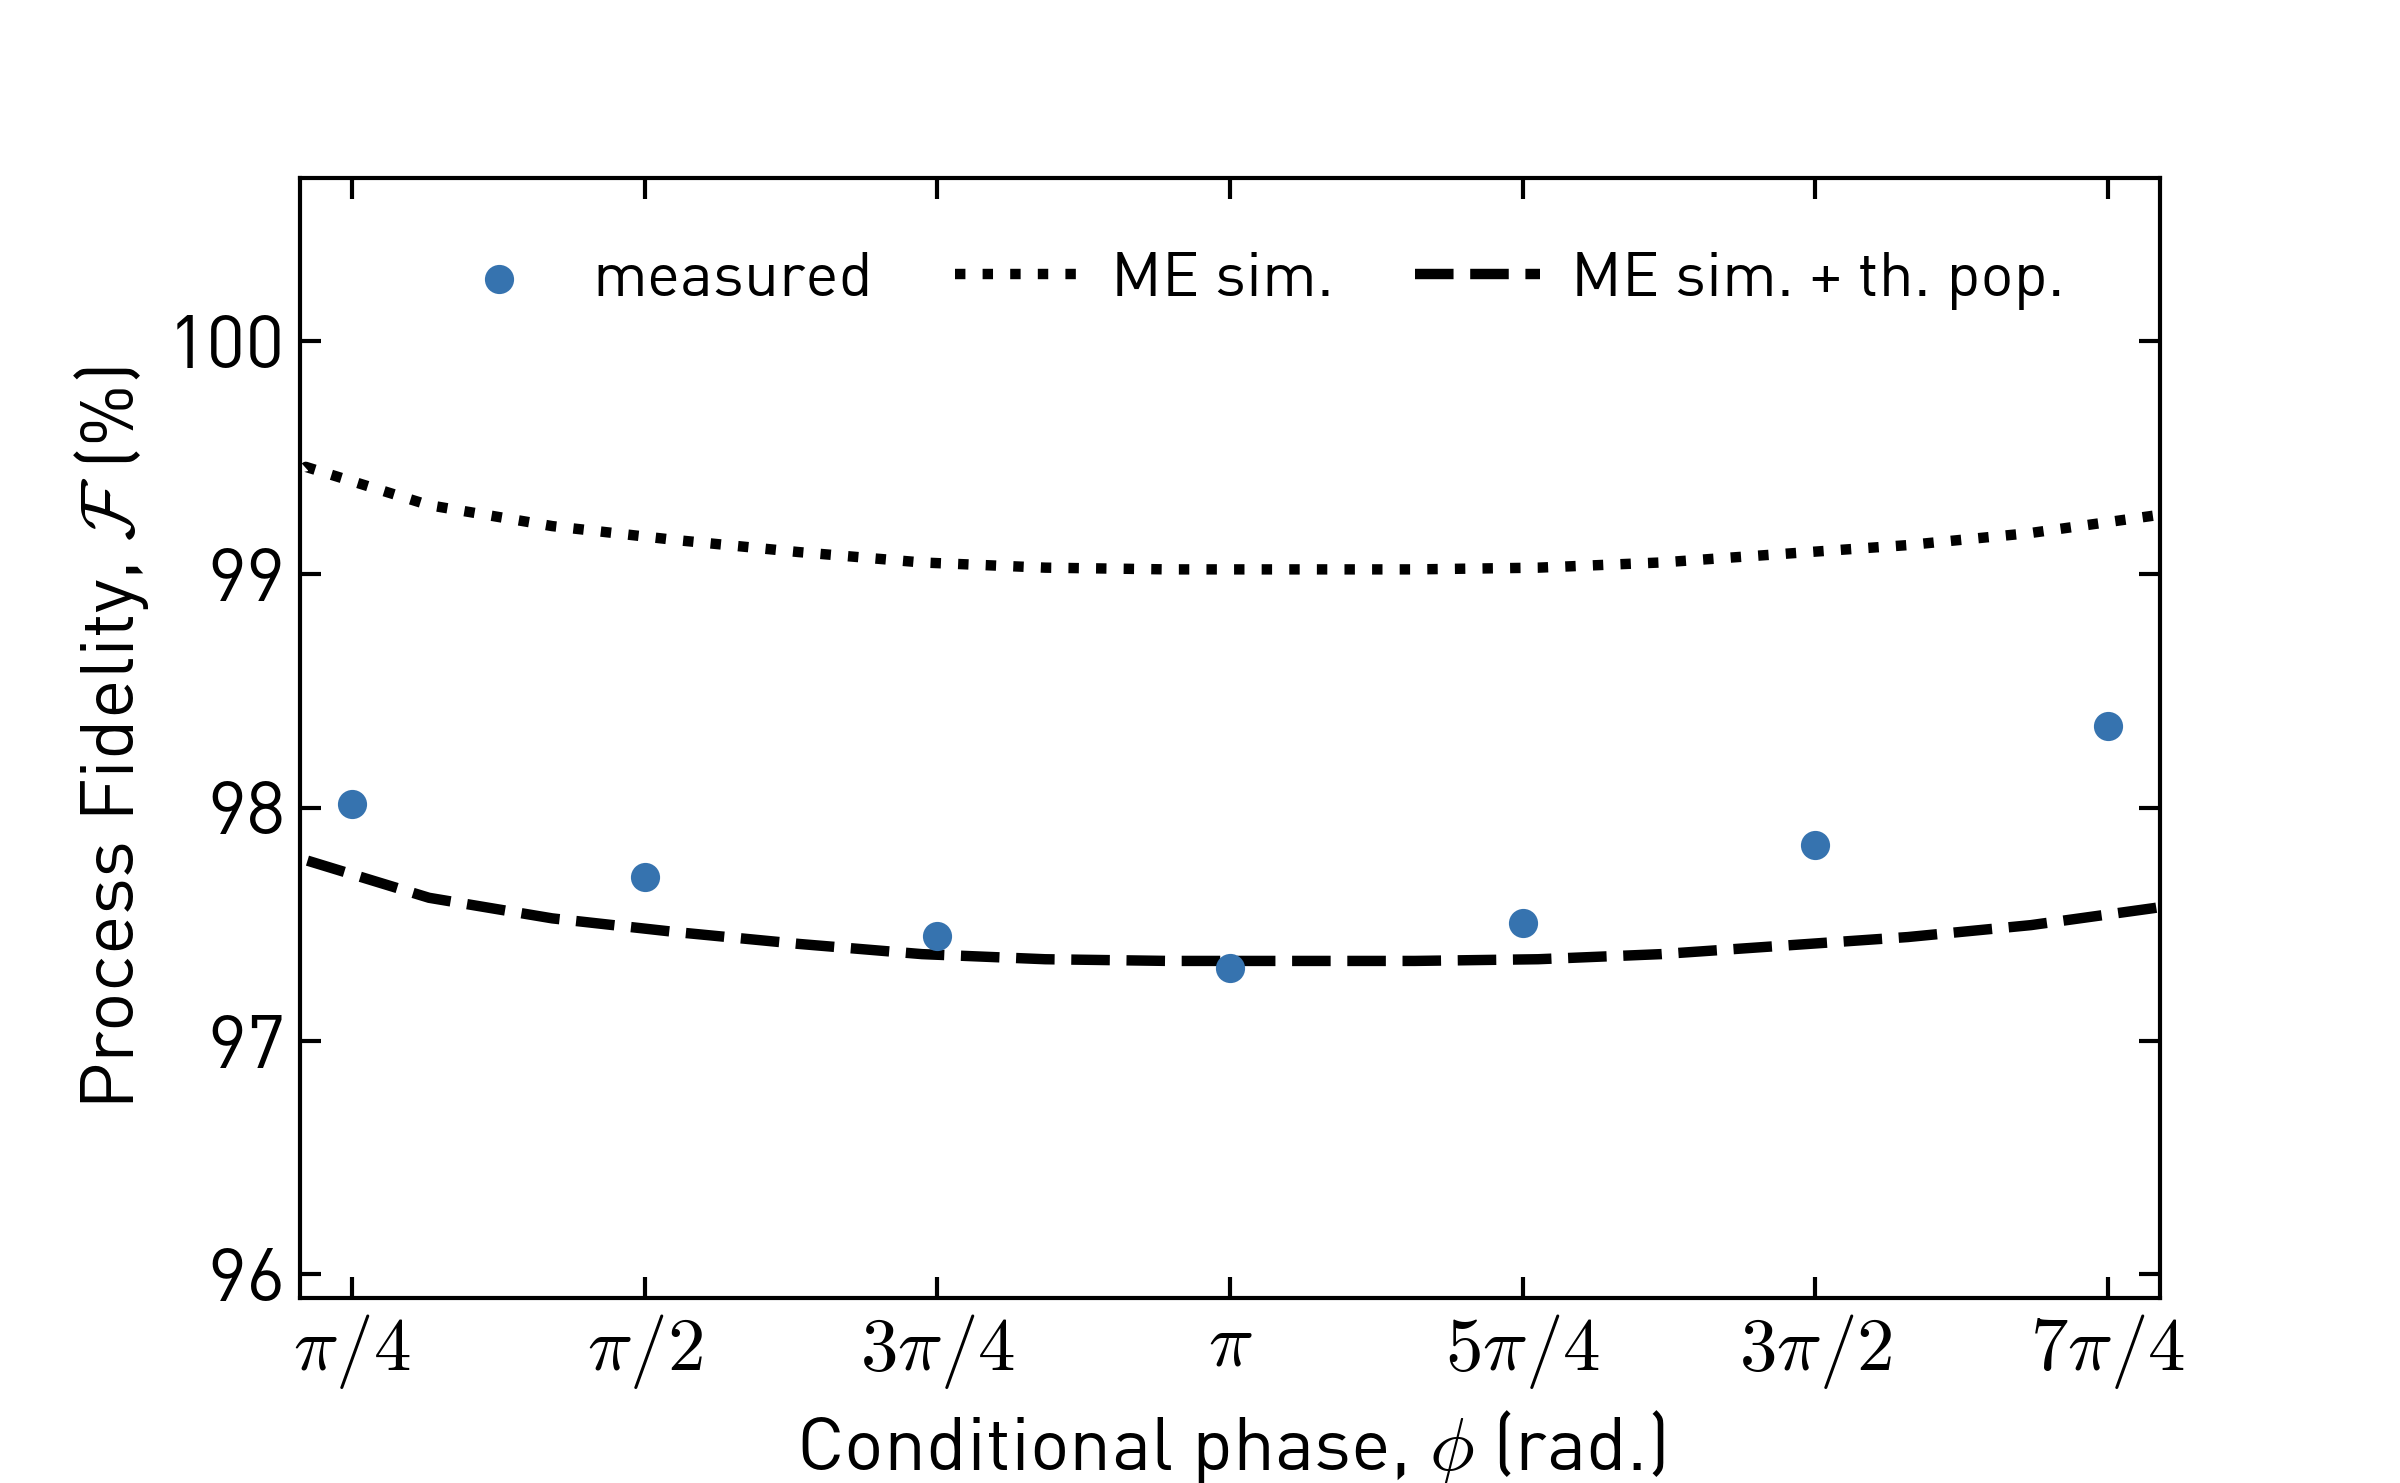
\includegraphics[width=\textwidth]{chapters/carb_gate/figs/ch4_characterization_tomo_all_angles_20200406_144758.png}
    \caption{Process fidelity as function of conditional phase angle of the \gls{carb}. Measurements are shown in scattered points.  Master equation simulation including effects of decoherence in dotted line. The dashed line corresponds to the fidelity of the simulation scaled by the probability of starting the measurement in the ground state. }
    \label{fig:carb_characterization_process_fidelity}
\end{figure}

Although \gls{qpt} yields full information of the quantum process, it also has several downsides. It is a time-consuming measurement and does not provide a direct and intuitive explanation about the different origin of errors. In addition, the maximum likelihood estimation of the process matrix relies on the assumption that state preparation and measurement errors are negligible, which is not necessarily the case when the length of the two-qubit pulse is on the same scale as the single-qubit tomography pulses (i.e. for small and large target conditional phases). Finally, it does not include information about leakage. We therefore perform additional characterization measurements in the next section which portray leakage and phase errors directly.

\subsection{Phases errors and leakage} \label{sec:carb_characterization_phase_errors_leakage}
A natural way to test the gate before its usage in an algorithm is to target a conditional phase and assess how close the measured conditional phase is from the target. When using 3-level readout, this measurement also characterizes, for each target phase, the \f{} level population of the qubit leaving the computational subspace (in this case, qubit 2). A similar approach allows to assess how well we are able to predict the dynamic phase the fluxed-qubit acquires.

We perform such a sweep over a target conditional phase in the range $[0\degree, 360\degree[$ with a spacing of 8\degree{} and present the results in Fig.~\ref{fig:carb_characterization_phase_errors_leakage}(a). The conditional (dynamic) phase error shows a distribution with mean and standard deviation of $0.23\pm0.97\degree$ ($-0.28\pm1.38\degree$) respectively. To reduce the phase error even further, we could investigate different interpolation strategies. However, we argue that these phase errors will not be the limiting factor when used in algorithms. Indeed, the fidelity\footnote{We use the  definition of fidelity between two pure states $\psi_{\rho}$ and $\psi_{\sigma}$ as the squared overlap between the amplitudes: $\mathcal{F} = \left|\left\langle\psi_{\rho} | \psi_{\sigma}\right\rangle\right|^{2}$~\cite{Jozsa1994FidelityStates}. We define the gate fidelity as by the fidelity between the state resulting for the ideal gate and the state resulting from the faulty gate implementation, minimized over all input
states~\cite{Reiner2018EffectsSystems}.} of a gate subjected to an over-rotation $\delta\phi$ degrades with $\cos^2{\delta\phi}$~\cite{Reiner2018EffectsSystems}. Therefore, for $\delta\phi = 2 \degree \approx 2\sigma_{\textrm{err}}$, the expected infidelity is on the order of $0.1\%$ ($0.2\%$ when adding both conditional and dynamic phase errors). By comparison, the effect of decoherence leads to a 5 times larger infidelity, and the 400\unit{kHz} residual $ZZ$-coupling for a duration of $100 \unit{ns}$ induces a phase error of 14.4\degree{} on the \oo{} state\footnote{Note that errors resulting from residual $ZZ$-coupling do not accumulate during the two-qubit gate but rather during single-qubit pulses and idle time because the calibration of the conditional phase includes the phase resulting from residual $ZZ$-coupling}. 

The leakage population shows an angular dependency. It is minimal ($P_f \approx 10^{-3}$) for conditional phases far from 180\degree, namely when the gate is short and the \oo{} and \tz{} states are off-resonant. By contrast, we observe leakage of up to $2\%$ when the \oo{} and \tz{} states are near resonance. At resonance, the population transfer is maximal, leading to a maximum in leakage population when assuming a fixed probability excitations being trapped in the \tz{} state. The dominant source of leakage are the short timescale distortions of the flux pulse~\cite{Rol2019Time-domainProcessor} which are not perfectly compensated by the \gls{fir} filters used for pre-distortion~\cite{Butscher2018ShapingFiltering}.  Leakage of qubit 3, which does not go into the \f{} level during the pulse, is on the order of $10^{-4}$ for all target conditional phases.

\begin{figure}[ht]
    \centering
    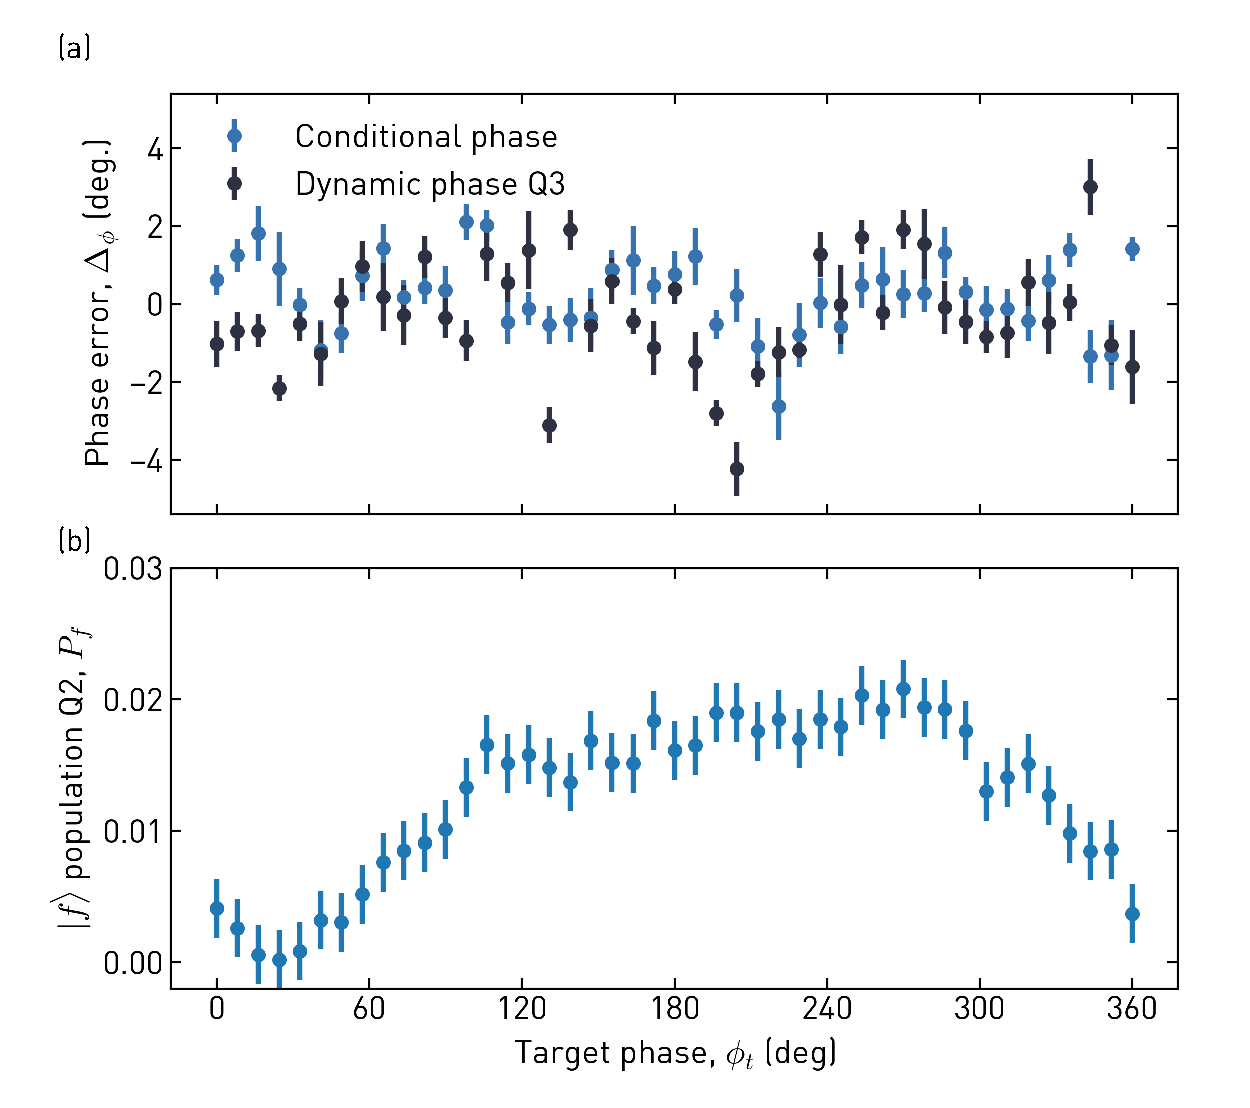
\includegraphics[width=\textwidth]{chapters/carb_gate/figs/ch4_characterization_phase_error_and_leakage_20200126_094856.pdf}
    \caption{Characterization of phase errors and leakage as function of target conditional phase with a granularity of 8\degree. Each point is averaged over 40000 single shots. (a) Conditional (light blue) and dynamic phase error (dark blue) show distributions with mean and standard distributions of $0.23\pm0.97\degree$ and  $-0.28\pm1.38\degree$ respectively. (b) We use 3-level readout to characterize leakage and measure up to 2\% leakage.}
    \label{fig:carb_characterization_phase_errors_leakage}
\end{figure}

\subsection{Comparison between C-ARB gates and CZ gates}
As final characterization procedure, we compare the \gls{carb} and \gls{cz} (implemented on the same qubits) in terms of phase errors, leakage and long term stability. We calibrate both gates and repeat the measurement described in Section~\ref{sec:carb_characterization_phase_errors_leakage}. For the \gls{cz}, we target a conditional phase of 180\degree, repeated $N$ times.  For the \gls{carb}, we sweep the range of target phases from 0 to 360\degree{} with $N$ points. These measurements are repeated for up to 15 hours after calibration. The full distributions of deviations from measured phases to target phases and leakages are presented as individual histograms, visualized as shaded filling in Fig.~\ref{fig:carb_characterization_drift}.

Both gates exhibit a similar range of conditional phase errors (standard deviation of $0.95\degree{}$ for the \gls{carb} versus $0.80\degree{}$ for the \gls{cz}). We conclude that extending the \gls{cz} to a \gls{carb} does not strongly impact the ability of preparing a target conditional phase. Note that the \gls{cz} shows a consistent offset of approximately 1\degree{} with respect to its target conditional phase. This originates from the fact that the gate is calibrated with a single point, which in this case was on the lower tail of the distribution. 

The \gls{carb} displays a wider distribution of dynamic phase errors, with an average standard deviation of 1.26\degree{} versus 0.83\degree{} for the \gls{cz}. This suggests it is harder to calibrate the dynamic phase for many flux pulse amplitudes and lengths simultaneously compared to calibrating only one. Preliminary analysis also suggest that the interpolation method has an influence on the standard deviation of the dynamic phase error. Using a cubic spline interpolation could help reduce the dynamic phase interpolation errors, compared to the implemented linear interpolation. 

The qubit 2 leakage trends are consistent with the discussion in Section~\ref{sec:carb_characterization_phase_errors_leakage}: the \gls{cz} experiences an average leakage of approximately 2\% since the \oo{} and \tz{} levels are on resonance. By contrast, the \gls{carb} experiences an average leakage of 1.4\% as several conditional phases result in low leakage. Its worse case leakage, however, is comparable to the one of the \gls{cz}. 

The phase error distributions stay relatively stable in time for both gates which suggests they will provide stable performance in algorithms for up to 15 hours after calibration.

The gates also differ in their average lengths. This effect is best visualized in Fig.~\ref{fig:ch4_calibration_carb}(a). While the \gls{cz} has a fixed flux pulse length of $107\unit{ns}$, the \gls{carb}'s flux pulse length is target phase dependent.  Averaged over all conditional phases, the flux pulse length is $84\unit{ns}$ long or $\sim 20\%$ shorter than for a conditional phase of 180 \degree. For both implementations, we add a $10\unit{ns}$ ($15\unit{ns}$) buffer at the start (end) to avoid overlap of other gates with the rising and falling edges of the flux pulse.

\begin{figure}[ht]
    \centering
    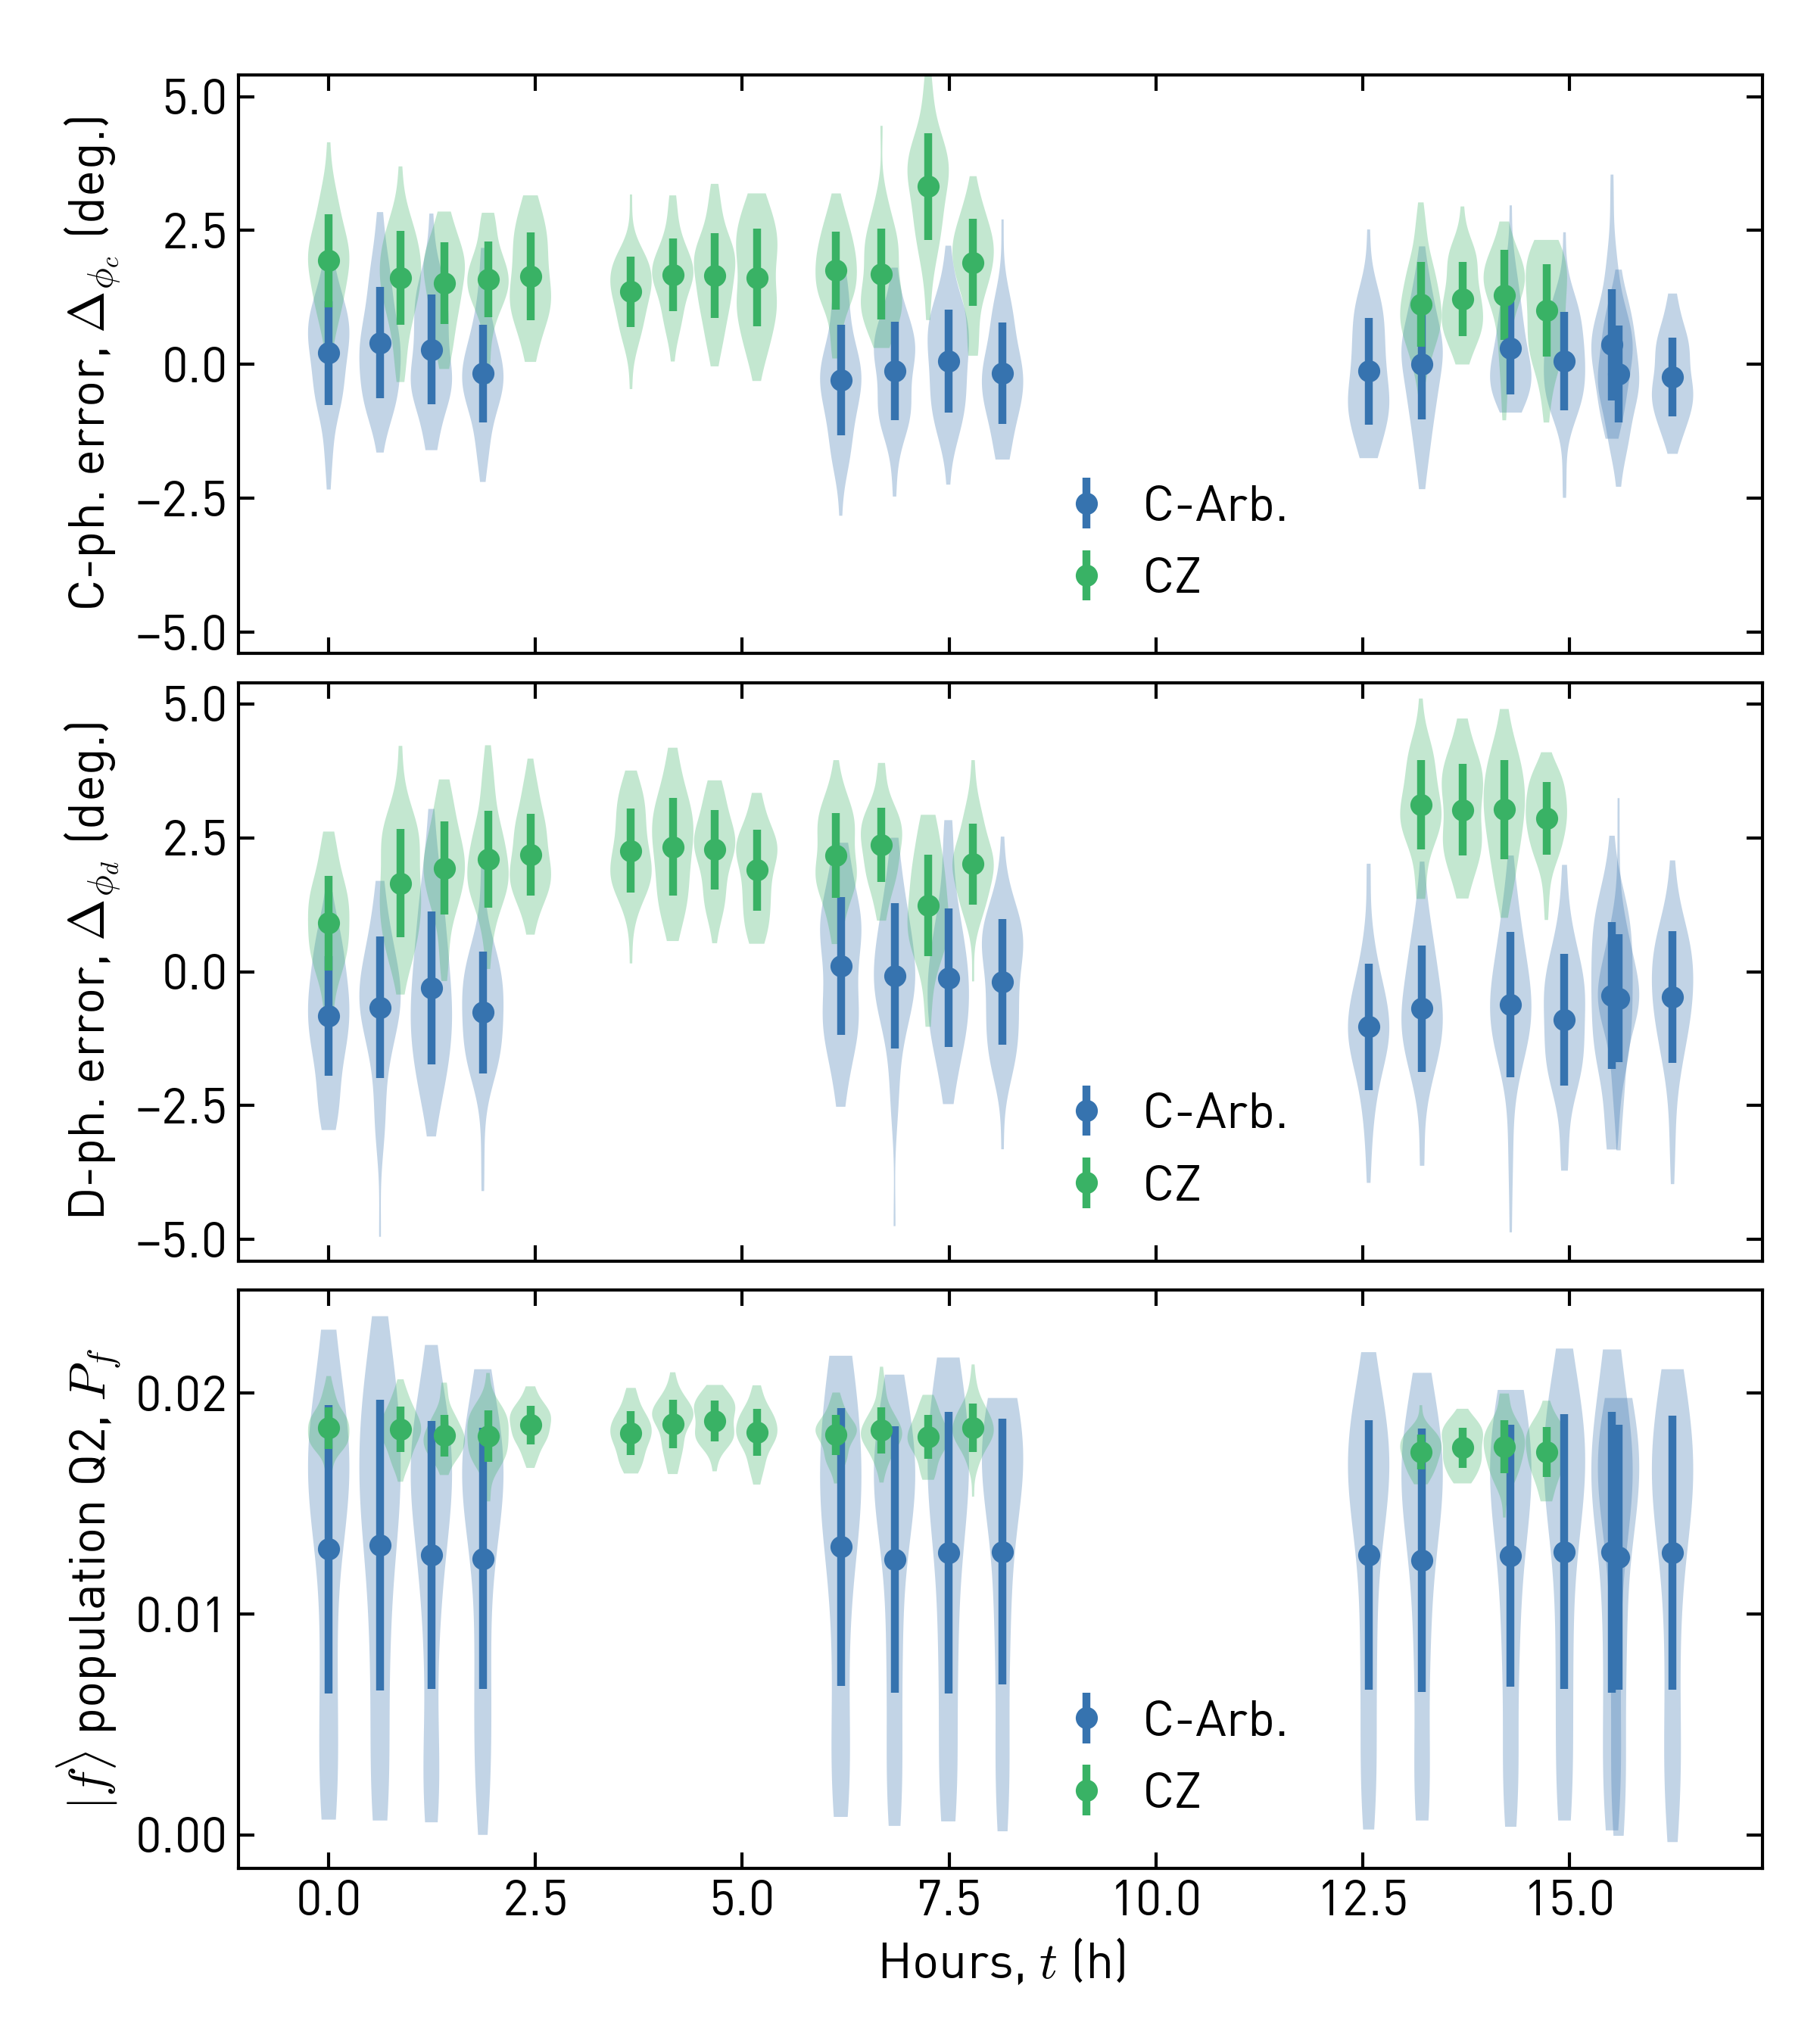
\includegraphics[width=\textwidth]{chapters/carb_gate/figs/ch4_characterization_drift_20200124_175455.png}
    \caption{Comparison between the \gls{cz} (green) and \gls{carb} (blue) in terms of phase errors and leakage as a function of time elapsed since calibration. The error bars correspond to the mean and standard deviation while the full distribution ($N$ = 45 points) is shown as shaded filling.}
    \label{fig:carb_characterization_drift}
\end{figure}

\section{Conclusion}
 In this chapter we have shown how to achieve a two-qubit unitary operation $U_{\textrm{C-ARB}}$ which adds an arbitrary phase $\phi$ on the \oo{} state. We implement this unitary by varying the frequency detuning between the \oo{} and the non-computational \tz{} state with a square,  Gaussian-filtered flux pulse. We adjust the length of the flux pulse to ensure high population recovery in the computational subspace. In practice, we calibrate the gate for a finite number of conditional phases (45) and interpolate linearly all parameters to reach phases between the calibration points. 
 
 We have characterized the gate using quantum process tomography for different conditional phases yielding a fidelity between 97.3\% and 98.3\%. The infidelity is dominated by decoherence and thermal population. In addition, we have shown that phase errors are small compared to other error mechanisms such as decoherence and residual $ZZ$-coupling. The average leakage amounts to 1.4\% and originates from the distortions of the flux pulse which are not corrected by the finite impulse response filter. The \gls{carb} shows similar time stability and phase error distributions as a \gls{cz} implemented on the same qubits while being 20\% shorter on average. 
 
 Although its calibration procedure is more elaborate, the \gls{carb} enables a significant gate count reduction for of \gls{vqa} circuits. In the next chapter, we implement a three-qubit problem instance which we solve using the \gls{qaoa} to demonstrate this advantage.



\chapter{Solving an exact cover problem instance using the QAOA} \label{ch:qaoa}
\glsreset{qaoa}
In this chapter, we first introduce combinatorial optimization. Next, we explain the \gls{qaoa}, a quantum heuristic algorithm providing approximate solutions to combinatorial optimization problems. We show that using \glspl{carb} can reduce the length of a \gls{qaoa}'s gate sequence implemented on the quantum computer. Next, we demonstrate this advantage experimentally by solving an exact cover problem instance on a three-qubit quantum processor.

\section{Combinatorial optimization}
An optimization problem for which the aim is to find the optimal (or close to optimal) solution amongst a finite set of possibilities is called a \textit{combinatorial optimization problem}.  Such problems are pervasive and appear in applications such as logistics, hardware verification, telecommunication network design, task scheduling and many more~\cite{Sbihi2007CombinatorialA, Coles2018QuantumBeginners, 2014ApplicationsOptimization}.

In its general form, a combinatorial optimization problem is specified by a set of rules, called clauses, acting on strings of $N$ bits, in which each bit represents a binary decision variable~\cite{Farhi2014AAlgorithm}.  Each clause is satisfied for certain assignments of the bits and unsatisfied for other assignments. Solving the problem consists in finding a combination of bits (forming together the bit string, $b := b_1 \, ...\, b_N$) satisfying the largest (weighted) amount of clauses. The objective function can be written as 
\begin{equation} \label{eq:qaoa_clauses}
    C(b) = \sum_{m=1}^M w_m C_m(b)
\end{equation}
where $C_m(b)$ is the $m$-th clause and $w_m$ is its corresponding (real and non-negative) weight. If $C_m(b)$ is satisfied by the bit string $b$ then its value is 1 and otherwise 0. In these terms, solving the problem is expressed as finding the bit string $b_\text{opt}$ maximizing $C$. An approximate solution provides a bit string $b_{\text{approx}}$ for which  $C(b_{\text{approx}})$ is close to the maximum of $C$.

We illustrate this abstract concept with a simple example. Imagine you  have to choose an outfit -- consisting of one t-shirt and one pair of pants -- from your closet. You have 2 shirts to choose from, a white and blue one. Similarly, you have a white and a blue pair of pants. You believe you look better when your whole outfit is of the same color. Additionally, you think your blue shirt suits you better than the white one. Which outfit should you choose for the party? 

While the answer is trivial in this example, we formalize the problem with the terminology introduced above. The outfit, $b = b_1b_2 $, can be formulated as a 2-bit string, one bit for the shirt ($b_1$), and one for the pair of pants ($b_2$). Colors are encoded by the values of the bits: 0 for white and 1 for blue. The four possible outfits are: 00 (white-white), 01 (white-blue), 10 (blue-white) and 11 (blue-blue). The problem has two clauses. $C_1(b) = \neg (b_1 \oplus b_2)$, leading to a value of 1 if you choose a shirt and pair of pants of the same color and 0 otherwise\footnote{$\oplus$ denotes the "XOR" operation and $\neg$ is the logical not.}. $C_2(b) = b_1$ has a value of 1 only if you decide on wearing your blue shirt. The objective function is then:
\begin{equation}
    C(b) = C_1(b) + C_2(b) = \neg (b_1 \oplus b_2) + b_1
\end{equation}
where we assigned equal weights $w_1 = w_2 = 1$ to both clauses.
The score of each output is then:
\begin{subequations}
\begin{equation}
     C(00) = 1 + 0 = 1
\end{equation}
\begin{equation}
    C(01) = 0 + 0 = 0
\end{equation}
  \begin{equation}
      C(10) = 0 +  1 = 1
  \end{equation}
  \begin{equation}
         C(11) = 1 + 1 = 2
  \end{equation}
\end{subequations}

The bit string maximizing $C(b)$ is indeed 11 (blue shirt, blue pants). An algorithm capable of providing this bit string is a combinatorial optimization algorithm. In this case, we used the exhaustive search algorithm, meaning that we enumerated all possible answers and picked the best one. 

In many real applications, exhaustive search is not tractable. In fact, even a slight modification of the presented problem makes it unrealistic to use exhaustive search. Instead of 2, imagine having to choose 25 items, each available in 8 different colors (each item has now 3 bits to encode the colors). The number of possible outfits becomes $2^{3 \cdot 25} \approx 4\cdot 10^{22}$. It would take about a million years to search sequentially through all possibilities for a computer requiring $1\unit{ns}$ to evaluate the cost of each outfit\footnote{Note that you are confronted to a similar situation every morning when dressing up. But you do not use the exhaustive search algorithm to decide what you wear, otherwise you would never get out of your house.}.

Several (classical) heuristic algorithms exist providing an approximate solution for this type of problems. In the next section, we explain the \gls{qaoa}, a quantum heuristic algorithm capable of finding approximate solutions to this type of problems.

\section{The quantum approximate optimization algorithm}\label{sec:qaoa}
The \gls{qaoa}~\cite{Farhi2014AAlgorithm} (depicted in Fig.~\ref{fig:qaoa_scheme}(a)) is a \gls{vqa} designed to find approximate solutions to combinatorial optimization problems. It is a hybrid algorithm executed partially on a quantum computer and partially on a classical computer. 

First, the quantum computer prepares a quantum state $\ket{\vec{\gamma}, \vec{\beta}}$ based on the objective function\footnote{Also often named cost function in the context of a minimization problem.} $C$ characterizing the clauses of the problem (see Eq.~\eqref{eq:qaoa_clauses}), and a set of variational parameters $\theta = (\vec \gamma, \vec \beta)$. The state is prepared with $p$ layers of two unitaries corresponding to the time-evolution of two non-commuting Hamitltonians, $\hat C$ and $\hat B$, applied to a uniform superposition state of $N$ qubits,
\begin{equation}
    |\vec{\gamma}, \vec{\beta}\rangle=\underbrace{\sexp{-\i \beta_{p} \hat B} \sexp{-\i \gamma_{p} \hat C}}_{\text {layer } p} \cdots \underbrace{\sexp{-\i \beta_{1} \hat B} \sexp{-\i \gamma_{1} \hat C}}_{\text {layer } 1}|+\rangle^{\otimes N}
\end{equation}
where  $\ket{+}^{\otimes N} = \left(\frac{1}{\sqrt{2}}(\ket{0}+\ket{1})\right)^{\otimes N}$ is the initialization state, and $\vec\gamma = (\gamma_1, ..., \gamma_p)^\text{T}$ and $\vec\beta = (\beta_1, ... , \beta_p)^\text{T}$ are the real variational parameters for the $p$ layers. Referring to the number of layers, we say that the implementation is of depth $p$. $\hat C$ is the cost Hamiltonian, which for all objective functions of NP-complete problems can be mapped to an Ising Hamiltonian in polynomial time~\cite{Lucas2014IsingProblems},
\begin{equation} \label{eq:ising}
    \hat C =\sum_{n < m} J_{n m} \sigma_{n}^z \sigma_{m}^z + \sum_{n} h_n \sigma_{n}^z
\end{equation}
and $\hat B$ is the mixing Hamiltonian 
\begin{equation}
    \hat B = \sum_{n} \sigma_n^x
\end{equation}
where $\sigma_n^{z}$ ($\sigma_n^{x}$) are the Pauli Z (X) operators applied to the $n$-th qubit, and $h_n$ and $J_{n m}$ are real coefficients. In the combinatorial optimization picture, these coefficients represent the relative weights of each clause, see Eq.~\eqref{eq:qaoa_clauses}.

\begin{figure}[H]
    \centering
    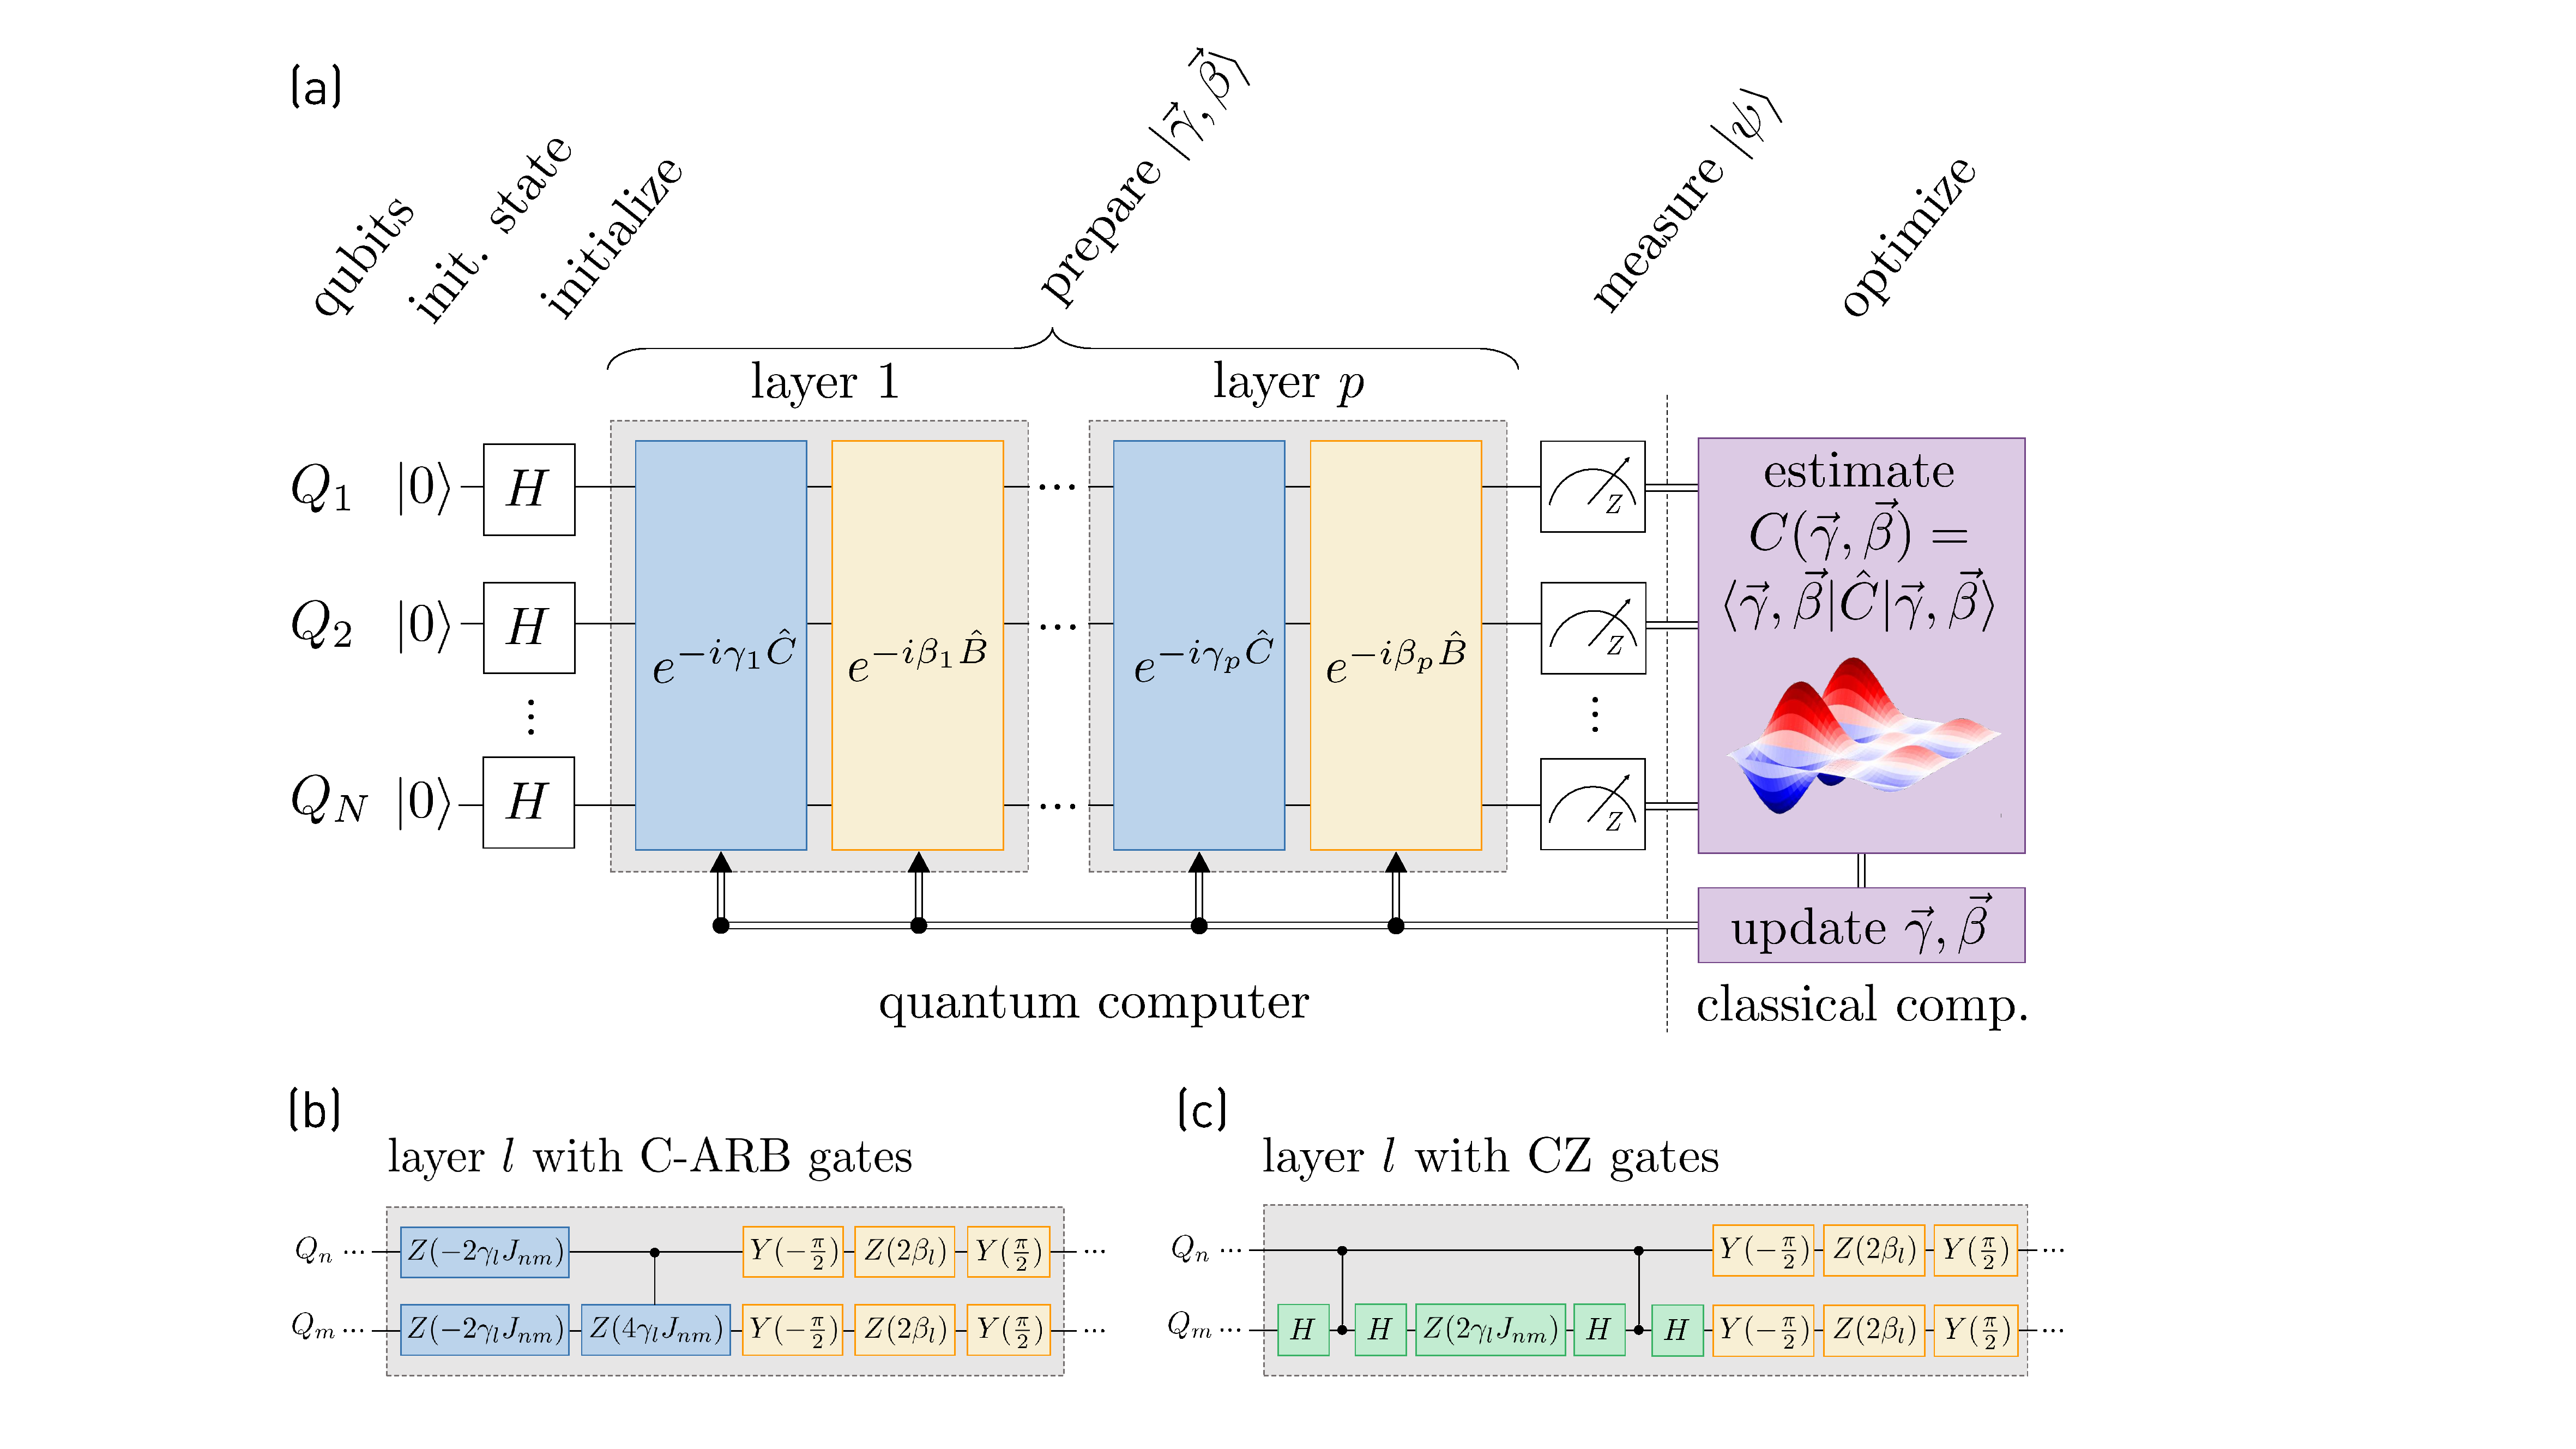
\includegraphics[width=\textwidth, trim ={9cm, 0 15cm, 0}]{chapters/qaoa/figs/qaoa_scheme-v6.pdf}
    \caption{The \gls{qaoa} scheme. $Z(\cdot)$ and $Y(\cdot)$ correspond to single-qubit z- and y-rotations while $H$ is the Hadamard gate. (a) The scheme consists of two steps. First, the quantum computer applies $p$ alternating sequences -- called layers -- of two unitaries corresponding to the time evolution of two Hamiltonians $\hat C$ (blue), $\hat B$ (yellow) scaled by layer-dependent variational parameters to an equal superposition state. The resulting state, \qaoaMeasuredState, is prepared and measured several times to obtain an estimate for the expectation value of a cost function \cost{}, based on the expectation values of single and two-qubit terms. Based on this estimate, a classical optimizer alters the variational parameters to minimize \cost{}. The output of the algorithm is the projection in the z-basis of state \optimalstate{} yielding a bit-string with a low cost. (b) Implementation of a layer of the \gls{qaoa} for a cost Hamiltonian consisting only of two-qubit interaction terms. Only two generic qubits, $Q_n$ and $Q_m$, are represented. The gate's background color indicates which part in (a) it implements. The single-qubit Z gates are virtual gates implemented by adding phase on the subsequent pulses. The two-qubit interaction is mediated by a \gls{carb}. The arbitrary single-qubit x-rotations are not calibrated on the device and are thus decomposed into two y-rotations and a z-rotation. (c) Equivalent gate sequence diagram as in (b) but featuring a decomposition of the \gls{carb} into \glspl{cz} and single-qubit gates.}
    \label{fig:qaoa_scheme}
\end{figure}

The resulting state \qaoaMeasuredState{} is measured in the $Z$ basis. A classical computer uses the measurement outcome (i.e.\ bit strings corresponding to the eigenstates of \qaoaMeasuredState{}) to compute the expectation value of $\hat C$ and iteratively updates the variational angles to optimize the objective function. When the objective function is mapped to the Ising Hamiltonian, the resulting problem consists in finding the lowest energy state of the system, i.e.\ minimizing the expectation value of the cost Hamiltonian. Once the optimizer has converged, the state \optimalstate{} constitutes an approximate solution for the optimization problem.

\subsection{Success probability} \label{sec:qaoa_success_prob}
Measuring successive preparations of \optimalstate{} yields a distribution on the eigenstates $\ket{\psi_i}$.
We define the success probability, $P_s$, as the probability of measuring an eigenstate that is a solution to the combinatorial problem. 

Note that the optimization is performed on the smooth landscape of the objective function \cost{} and not on $P_s$ directly. But for problems with a discrete domain of real values, a low expectation value of the cost function generally guarantees a high concentration of probability on optimal solutions upon measurement~\cite{Cook2019TheCover, Wang2019XY-mixers:QAOA}.

\subsection{Layer implementation}
The algorithm is subdivided into layers, in which each layer $l$ includes the unitary $\sexp{-\i\gamma_l\hat C}$. Since $\hat C$ is diagonal in the computational basis, all its terms commute. In addition, in this thesis we consider the case where all $h_n = 0$. Therefore, we look at the implementation of a single generic term $J_{nm}\sigma_n^z\sigma_m^z$ involving qubit $Q_n$ and qubit $Q_m$. Any other term in $\hat C$ can be applied before or after in the exact same way. 

The corresponding unitary to implement is $\sexp{-\i J_{nm} \gamma_l \sigma_n^z\sigma_m^z}$, yielding in the $nm$-two-qubit subspace,
\begin{equation} \label{eq:qaoa_two_qubit_cost_unitary}
    U_{nm}^l = 
    \begin{pmatrix}
    \sexp{-\i\gamma_l J_{nm}} & 0 & 0 & 0\\
    0 & \sexp{\i\gamma_l J_{nm}} & 0 & 0 \\
    0 & 0 & \sexp{\i\gamma_l J_{nm}} & 0 \\
    0 & 0 & 0 & \sexp{-\i\gamma_l J_{nm}}
    \end{pmatrix}
\end{equation}{}
We present two approaches to implement this unitary. The first one, which we call the \textit{\gls{dir}}, implements Eq.~\eqref{eq:qaoa_two_qubit_cost_unitary} with a single \gls{carb} and two single-qubit $Z$-gates (see Fig.~\ref{fig:qaoa_scheme}(b)). The \gls{carb} introduces a phase of $4\gamma_l J_{nm}$ on the \oo{} state which is then redistributed to the other diagonal terms by single-qubit $Z$-gates rotating their respective qubit subspace in the opposite direction with half the angle, i.e.\ $2\gamma_l J_{nm}$. Up to a global phase, this implements Eq.~\eqref{eq:qaoa_two_qubit_cost_unitary}. Note that, due to the presence of the variational parameter $\gamma_l$, the angle on the \oo{} state may have any real value and therefore indeed requires a \gls{carb} to rotate the \oo{} state with a single gate.

In case we choose to limit the gate set to the use of \glspl{cz} only (i.e.\ rotation of $\pi$ on the \oo{} state), we use a \textit{\gls{dec} } consisting of two \glspl{cz} and additional single-qubit gates (see green colored elements in Fig.~\ref{fig:qaoa_scheme}(c)).

In Section~\ref{sec:qaoa_experiment}, we compare experimentally the performance of both implementations.

\subsection{Relation to adiabatic quantum computing}\label{sec:qaoa_relation_to_adiabiatic_computing}
The depth $p$ of a \gls{qaoa} implementation is defined as the number of layers used for the state preparation. This parameter plays an important role both in theory and in experiments.

For $p \rightarrow \infty$, the \gls{qaoa} finds the global optimium of $C$~\cite{Farhi2014AAlgorithm}. Intuitively, this is because the \gls{qaoa} can be seen as a Trotterized approximation~\cite{TrotterMathematics} of the quantum adiabatic algorithm~\cite{Farhi2000QuantumEvolution}. Similarly to the \gls{qaoa}, the quantum adiabatic algorithm starts in the lowest energy state of the mixing Hamiltonian $\hat B$, i.e.\ the equal superposition over all qubits in the $Z$ basis, and then evolves adiabatically to the lowest eigenstate of the cost Hamiltonian $\hat C$. The time-dependent Hamiltonian during this evolution is

\begin{equation} \label{eq:qaoa_adiabatic_evolution}
 \hat H(t)=\hat H_1(t) +\, \hat H_2(t) = (1-t / T) \hat B + \, (t / T) \hat C
 \end{equation}
where $T$ is a real and positive parameter called run time. As long as the evolution is sufficiently slow i.e.\ $T$ is sufficiently large, this process forces the state of the system to remain in the ground state of the slowly varying Hamiltonian $\hat H(t)$, ultimately resulting to the ground state of $\hat C$~\cite{Farhi2000QuantumEvolution, Farhi2014AAlgorithm}. 

To implement this on a quantum computer, we break down the total time evolution $U(0, T)$ from 0 to $T$ into $K$ smaller intervals $U_k((k-1)\Delta t,\, k\Delta t)$ of length $\Delta t$ such that
\begin{equation} \label{eq:qaoa_discretized_adiabatic_evolution}
    \ket{\psi_{\textrm{opt}}} = U(0, T)\ket{+}^{\otimes N} = U_K((K-1)\Delta t, \,K\Delta t) ... U_0(0,\, \Delta t) \ket{+}^{\otimes N}
\end{equation}
with the time evolution in each interval given by 
\begin{equation}
    U_k(k\Delta t, (k+1)\Delta t) = \mathcal{T}\exp{\left(-\i\int_{k\Delta t}^{(k+1)\Delta t} \hat H(t)\d t\right)}
\end{equation}
 and the time ordering operator $\mathcal{T}$~\cite[p. 143]{Weinberg1995TheFields}. It is shown that removing the time ordering operator introduces an error $\epsilon \propto \Delta t^2$~\cite{Poulin2011QuantumSpace}. Intuitively, this suggests that as long as the time intervals are small, the order of operations within the step leads to negligible errors. It is also more practical to approximate the integral by a sum, for instance using Monte-Carlo integration~\cite{Poulin2011QuantumSpace}. The latter replaces the integral by the average of $M$ evaluations of the function at random times $\tau_m^k$ within the interval $\Delta t$ which introduces an error $\epsilon_{\textrm{MC}} \propto \Delta t/\sqrt{M}$. The time evolution step becomes
 \begin{equation}
     U_k(k\Delta t, (k+1)\Delta t) = \exp{\left(-\frac{\i}{M}\sum_{m=1 }^{M} \hat H(\tau_m))\right)} =  \prod_{m=1}^M \sexp{-\frac{\i}{M}\hat H(\tau_m^k)}
 \end{equation}
 Within the product, the Hamiltonian is not time dependent anymore, such that we can apply the Trotter formula to decompose it into the two components $\hat B$ and $\hat C$. 
 The Trotter product formula stipulates for two non-commuting time-independent Hamiltonians $\hat H_1$ and $\hat H_2$~\cite{TrotterMathematics}:
\begin{equation} \label{eq:qaoa_product_formula}
    \sexp{-\i\left(\hat H_{1} + \hat H_{2}\right) t}=\lim _{N \rightarrow \infty}\left(\sexp{-\i \hat H_{1} t / N} \sexp{-\i \hat H_{2} t / N}\right)^{N}
\end{equation}
Truncating this equation to a finite value for $N$ yields an error with lowest order term in $\mathcal{O}\left(\frac{t^2}{2N} [\hat H_1, \hat H_2]\right)$~\cite{Heyl2018QuantumSimulation, Lloyd1996UniversalSimulators}. 

In this case, we make an approximation of order $N=1$ with $\hat H_1 = (1-\frac{\tau_m^k}{T})\hat B$ and $\hat H_2 = \frac{\tau_m}{T} \hat C$. The full adiabatic evolution of Eq.~\eqref{eq:qaoa_discretized_adiabatic_evolution} becomes the alternating sequence between the two Hamiltonians $\hat B$ and $\hat C$,
\begin{equation} \label{eq:qaoa_prod_formula}
    U(0,T) = \prod_{k=0}^{K-1} U_k(k\Delta t, \,(k+1)\Delta t)= \prod_{k=0}^{K-1}\prod_{m=1}^M \sexp{-\i\frac{ \overbrace{1-\tau_m^k/T}^{\beta_{km}}}{M}\hat B}\sexp{-\i\frac{\overbrace{\tau_m^k/T}^{\gamma_{km}}}{M}\hat C}
\end{equation}
Note that applying this discretized adiabatic time evolution on $\ket{+}^{\otimes N}$ as presented in Eq.~\eqref{eq:qaoa_discretized_adiabatic_evolution} ends in the global extremum of $\hat C$ \textit{only} for $K \rightarrow \infty$ and large $T$. In that case, the number of layers is given by $p = K\cdot M$ and corresponds intuitively to approximating the time evolution from 0 to $T$ by infinitely many time steps. The error in the approximation of the integral intrinsically tends to zero if $\Delta t \rightarrow 0$. In such a scenario, the  set of variational parameters $(\vec\gamma, \vec\beta) = \{(\gamma_0, \beta_0), ... (\gamma_p, \beta_p)\}$ highlighted in Eq.~\eqref{eq:qaoa_prod_formula} suffices to find the optimum. 

However, in practice the number of layers we can implement on a quantum computer is limited. Therefore, we truncate Eq.~\eqref{eq:qaoa_prod_formula} to a finite value for both $K$ and $M$. This truncation introduces approximation errors and finding the global optimum is no longer guaranteed. 

To mitigate this approximation, we relax the adiabatic constraint ($\beta_l = 1 - \gamma_l$) at each layer to allow for a potentially more direct path to the ground state than the adiabatic one. By optimizing these parameters at each layer variationally, the \gls{qaoa} can reach the ground state with high accuracy for some problem instances even with a relatively small number of layers~\cite{Moll2017QuantumDevices}. 

\subsection{Quantum speedup and the importance of depth}
At the time of its first publication, the \gls{qaoa} achieved a higher approximation ratio on MAX-3-LIN-2 -- a specific instance of the NP-complete MaxCut problem~\cite{GareyM1990} -- than any other classical algorithm. This is no longer the case~\cite{Barak2015BeatingDegree, Hastings2019CLASSICALALGORITHMS}. In fact, several research articles have shown that classical algorithms could outperform the \gls{qaoa} on a variety of problem instances~\cite{Barak2015BeatingDegree, Hastings2019CLASSICALALGORITHMS, Bravyi2019ObstaclesProtection}. On the other hand, several articles claim to achieve Grover speedup for unstructured search~\cite{Jiang2017Near-optimalField} and state transfer~\cite{Niu2019OptimizingDepth} using the \gls{qaoa}. Whether or not the \gls{qaoa} will provide a provable or practical speedup compared to classical algorithms remains unanswered. 

Understanding the number of layers required to open a path to the ground state as function of (i) the number of qubits in the Hamiltonian, and (ii) the chosen problem instance are both open research questions. In addition, it remains unclear whether the path can be found efficiently as the number of variational parameters grows with $2p$. Early results suggests that, for \gls{qaoa} to provide any quantum speedup, the scaling of $p$ must be faster than $\mathcal{O}(1)$ otherwise the circuit is likely simulated efficiently on a classical computer~\cite{Bravyi2019ObstaclesProtection}. On the other hand, to ensure a quantum speedup the scaling of $p$ should also not grow faster than $\mathcal{O}(\log N))$ because faster scaling could imply that finding good variational parameters becomes exponentially hard~\cite{Cerezo2020Cost-Function-DependentNetworks}. 

While the above considerations provide insights into the theoretical performance of the \gls{qaoa} as function of depth, they do not provide insights into the experimental performance on \gls{nisq} devices. In this work, we highlight a crucial experimental trade-off related to the number of layers. Namely, in theory the performance of \gls{qaoa} circuits can only improve with increasing number of layers~\cite{ZhouQuantumDevices}. However, the performance on near-term quantum computers will not increase monotonically with depth due to decoherence and other noise sources. There will be an optimal number of layers beyond which additional layers only decrease the performance of the algorithm. We illustrate this trade-off in the next section and show that the \gls{dir} increases the number of layers which can be executed reliably compared to the \gls{dec}
This in turn allows to solve more complex problem instances using the \gls{dir}

\section{Exact cover} \label{sec:qaoa_exact_cover}
We choose to solve an instance of the exact cover problem~\cite{Karp1972ReducibilityProblems} to compare the direct and decomposed implementation of \gls{qaoa}. The exact cover is NP-complete~\cite{GareyM1990}, meaning that there is no known algorithm to find answers in polynomial time\footnote{An algorithm runs in polynomial time if its execution time, in the worst case scenario, is upper-bounded by a polynomial function of the input $N$, i.e.\ its time complexity scales as $\mathcal{O}(N^k)$ with $k$ a positive and real constant.}, but answers can be checked in polynomial time. In other words, the problem is "hard to solve" but it is "easy" to check the validity of a proposed solution. In addition, the NP-completeness guarantees that any problem in NP can be reduced to the exact cover in polynomial time, such that studying the exact cover is closely related to studying other NP problems. Finally, the exact cover can be easily construct via a problem graph that is not complete, which allows to create instances respecting the hardware connectivity of the quantum device (see Chapter~\ref{ch:outlook} for a discussion on hardware connectivity).

In this section, we provide the formal definition of the exact cover and introduce a problem instance which we the solve in Section~\ref{sec:qaoa_experiment} using \gls{qaoa}. 

\subsection{Definition}
The exact cover is an NP-complete decision problem formulated as follows: \textit{given a set $\mathcal{N}$, and a collection $\mathcal{L}$ of subsets of $\mathcal{N}$, is there a subcollection $\mathcal{L}'$ of $\mathcal{L}$ for which each element in $\mathcal{N}$ is included exactly once?} In other words, elements of the subcollection $\mathcal{L}'$ must be disjoint and their union must be $\mathcal{N}$.

As mentioned in Section~\ref{sec:qaoa}, any NP-complete problem can be mapped onto an Ising Hamiltonian in polynomial time. For the exact cover, this is most conveniently done using an incidence matrix $M$~\cite{WeissteinIncidenceMatrix}, where each row corresponds to an element of $\mathcal{L}$ and each column to an element of $\mathcal{N}$. The matrix element $M_{ln}$ is equal to 1 if the $l$-th element of $\mathcal{L}$ contains the $n$-th element of $\mathcal{N}$ and 0 otherwise.
The Ising parameters $J_{nl}$ and $h_l$ are obtained from $M$~\cite{Lucas2014IsingProblems, Vikstal2019ApplyingProblem}:
\begin{subequations}
\begin{equation}
    J_{l n}=\frac{1}{2} \sum_{k=1}^{N} M_{l k} M_{n k}
\end{equation}
\begin{equation}
h_{l}=\frac{1}{2} \sum_{n=1}^{N} M_{l n}\left(\sum_{k=1}^{L} M_{k n}-2\right)
\end{equation}
\end{subequations}
This formulation requires $L = |\mathcal{L}|$ binary variables $\{b_1, ..., b_L\}$ with $b_l\in\{0,1\}$. To yield an Ising Hamiltonian formulation, see Eq.~\eqref{eq:ising}, each binary variable $b_l$ is mapped to a spin variable $\sigma_l \in \{-1,1\}$ with the mapping, 
\begin{equation}
\sigma_l = 1 - 2 b_l
\end{equation}
Finally, each spin in the problem is modelled by a qubit on the quantum processor. 

\subsection{Example problem instance}
In this work, we consider the 3-qubit problem instance depicted in Fig.~\ref{fig:qaoa_exact_cover_matrix}.  $\mathcal{N} := \{1,2,3\}$ and the elements of $\mathcal{L}$ are $A := \{1,2\},\,\, B := \{1,2,3\}$ and $C := \{2,3\}$, encoded in qubit 1, 2 and 3 respectively. In this picture, the decision problem becomes: \textit{is there a subcollection $\mathcal{L}'$ of letters for which each number in $\mathcal{N}$ is included exactly once?} The answer is yes, and the corresponding subcollections are $\mathcal{L}_1' = \{A,C\}$ and $\mathcal{L}_2' = \{B\}$. These subcollections are encoded in the states $\ket{\psi}=\ket{101}$ and $\ket{010}$, where a 1 in position $l$ indicates that the $l$-th element of $\mathcal{L}$ is included in the subcollection $\mathcal{L'}$.

"Solving" this problem instance corresponds to measuring $\ket{\psi}=\ket{010}$ and $\ket{\psi}=\ket{101}$ with high probability as measuring and checking whether this state is part of the solution set would allow to answer the yes/no-decision problem.

The cost Hamiltonian of the problem is
\begin{equation}
    \hat C = \frac{1}{2}\hat\sigma_1^z\hat\sigma_2^z + \hat\sigma_2^z\hat\sigma_3^z
\end{equation}
and the corresponding cost function $\cost = \bra{\vec\gamma, \vec\beta} \hat C \qaoaMeasuredState{}$ reaches its minimum value of $\cost = -1.5$ when $\qaoaMeasuredState{} = \ket{101}$ or $\ket{010}$. 

\begin{figure}[t]
    \centering
    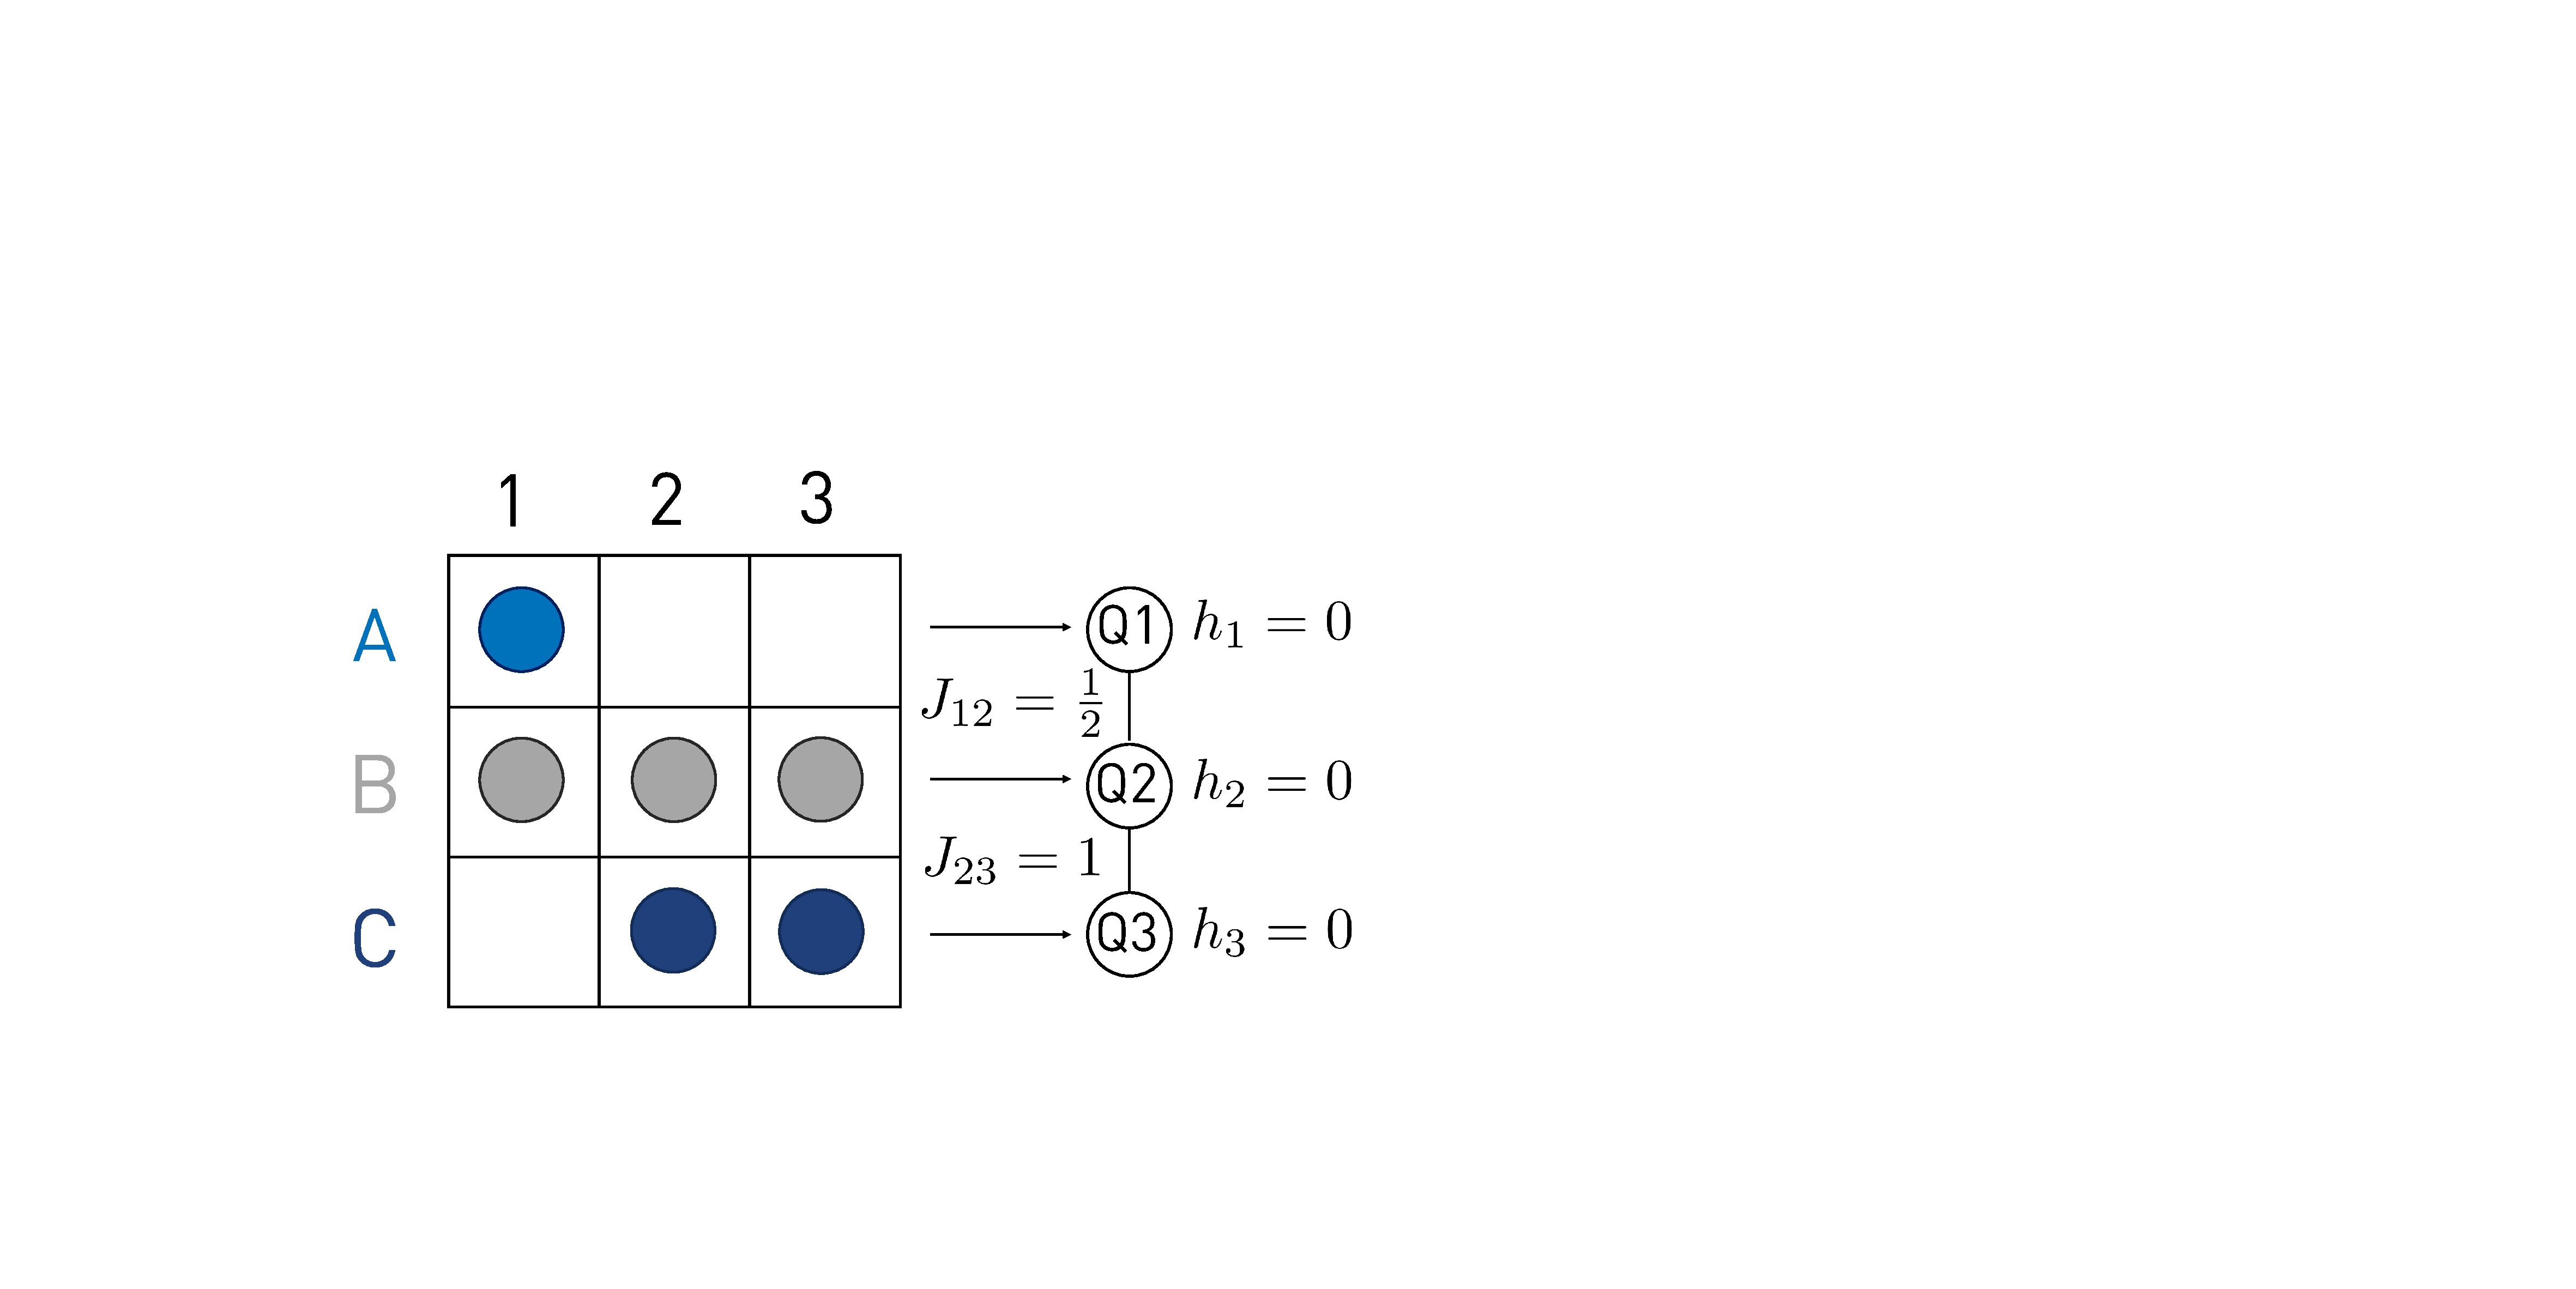
\includegraphics[width=0.8\textwidth, trim={11cm 8cm 38cm 13cm},clip]{chapters/qaoa/figs/exact_cover_matrix.pdf}
    \caption{Incidence matrix representation of the exact cover problem instance implemented in this work. A dot indicates a 1 and an empty square indicates a 0. The mapping to the 3 qubit chain and the corresponding Ising Hamiltonian parameters are indicated on the right hand side.}
    \label{fig:qaoa_exact_cover_matrix}
\end{figure}

\section{Experiment} \label{sec:qaoa_experiment}
In this section, we implement the \gls{qaoa} on a quantum processor to find an approximate solution to a combinatorial optimization problem with 3 qubits. In addition, we compare the performance of the \gls{dir} and \gls{dec} for different depths. We use qubits 1, 2 and 3 of the device presented in Appendix~\ref{app:setup}. Information relative to the single- and two-qubit gates are reported in Appendix~\ref{app:setup}, Table~\ref{tab:cz_gate_params}. All measurements are performed with 3-level single shot readout, see Appendix~\ref{ch:qutrit_readout}. In the context of the \gls{qaoa}, leakage events can be seen as measuring bit strings which do not belong to the space of possible solutions. We therefore condition the measurements outcome on no leakage event. Hence, leakage events reduce the effective number of shots on which we compute estimates. They do not, however, influence the algorithm as long as as the excitation stays in the \f{} level until the state is measured. We make this assumption, as sequences of interest are shorter than $4\,\mu\text{s}$, and the shortest \f{} level $T_1$ is approximately $10\,\mu\text{s}$. All measurements are done without ground state heralding or readout error correction.

\subsection{Cost function landscapes}
Although $p=1$ does not always yield a good approximate solution to the optimization problem, it is a useful intermediate benchmark towards implementing multi-layer \gls{qaoa} circuits ~\cite{Pagano2019QuantumSimulator, Bengtsson2019QuantumProcessor}. A single layer implementation has two variational parameters, $\gamma$ and $\beta$, such that the cost function landscape can be mapped out and visualized with a grid search over $\gamma$ and $\beta$. We make several observations to restrict the search space for each parameter. 

First, if $\hat C$ has only integer eigenvalues\footnote{$\hat C$ is diagonal and therefore elements on its diagonal are the eigenvalues by definition.}, then $\gamma$ is at least $2\pi$-periodic because $\sexp{-\i(\gamma + 2\pi) \hat C} = \sexp{-\i 2\pi \hat C} \sexp{-\i \gamma \hat C} = \sexp{-\i \gamma \hat C}$ since $2\pi \hat C$ yields integer multiples of $2\pi$ for all elements on the diagonal. If in addition the eigenvalues are either all odd or all even, then $\gamma$ shows a periodicity of $\pi$, as $\sexp{i\pi\hat C}$ yields in that case $\pm I$ depending on whether the eigenvalues are all odd or all even. By construction, this is the case when all $J_{nm}$ in $\hat C$ are integers. 

Second, the parameter $\beta$ yields single-qubit $x$-rotations of angle $2\beta$ on all qubits and is therefore at least $\pi$-periodic.

We thus restrict our search space for this problem instance\footnote{In the problem instance we study, the eigenvalues are odd integers multiples of 1/2 and not odd integers. Therefore, the periodicity in $\gamma$ is only $2\pi$ and not $\pi$. We make use of the fact that the landscape is point symmetric around ($\gamma$, $\beta$) = ($\pi$, $\pi/2$) due to the linear connectivity to restrict the search space of $\gamma$ between 0 and $\pi$. Another option would have been to multiply $\hat C$ by a constant factor such that all eigenvalues are integers.} to the domain $(\gamma, \beta) \in [0, \pi] \,\times\, [0, \pi]$. For each parameter pair, we repeat the state preparation and measurement 20000 times to estimate the expectations values $\langle\szsz{1}{2}\rangle$ and $\langle \szsz{2}{3} \rangle$ from which the cost \cost{} is computed.

We execute this measurement with a resolution of 45 points per axis both for the \gls{dir} and the \gls{dec}, and present the result in Fig.~\ref{fig:qaoa_landscapes} along with the landscape obtained with a noise-free unitary evolution (which does not take into account decay and dephasing rates) simulated in QuTip~\cite{Johansson2013QuTiPSystems} .

The simulation reveals two global minima for \cost{} $\approx -1.05$ at $(\gamma, \beta) \approx (\frac{2\pi}{9}, \frac{\pi}{7})$ and $(\frac{2\pi}{9},\pi/2 + \frac{\pi}{7})$.  The landscape also exhibits two pairs of local minima with slightly different depths; one at $\gamma \approx \frac{5\pi}{8}$ and one at $\gamma \approx \frac{7\pi}{8}$ also separated by $\pi/2$ in the $\beta$ direction. The $\pi/2$ periodicity in $\beta$ can be understood intuitively from the Bloch sphere perspective: for $p=1$, we start on the equator and apply parametrized entangling $Z$-rotation between qubits. Each qubit therefore stays on the equator of its Bloch sphere. Thereafter, we apply parametrized $X$-rotations on all qubits which rotate the vectors back towards the $z$-axis\footnote{Except if the vectors are degenerate with the $\pm x$-axis.}. For a $X$-rotation angle larger than $\pi$ (i.e.\ $\beta>\pi/2$), we simply inverse the polarity of all states (all $\ket{1}$ are now mapped to $\ket{0}$ and vice-versa). The correlations between qubits remain unaffected by this polarity inversion and therefore the landscape is periodic.

The locations of all extrema in the measurements are in good agreement with the simulations, suggesting a low amount of total coherent errors. Incoherent errors due to decoherence affect the contrast of the landscapes, resulting in a minimum measured cost of $\sim -0.95$ ($\sim -0.85$) for the direct (decomposed) implementation. The decomposed implementation does not reach the same cost value as its gate sequence is longer and thereby more affected by decoherence. In addition, it suffers more from coherent errors than the direct implementation. The latter are caused predominantly by residual $ZZ$-coupling, and therefore accumulate over the longer sequence. The combination of these effects could explain the diagonal feature observed in its landscape, which does not appear as strongly for the direct implementation. The average total leakage (any qubit measured in the \f-level) amounts to 4.5\% for the direct implementation and 7.8\% for the decomposed implementation. Most of the leakage occurs due to the two-qubit gate between qubit 1 and qubit 2, which suffers from higher leakage (see Appendix~\ref{app:setup}, Table~ \ref{tab:cz_gate_params} for a detailed discussion).

Note that even in the noise-free simulation, \cost{} never reaches its minimum value of -1.5 thereby indicating that the performance of the algorithm is limited by the chosen depth of $p=1$. Nevertheless, additional layers introduce new variational parameters, making grid search quickly intractable. Therefore, we use a classical optimizer to find the optimal variational parameters.

\begin{figure}[ht]
    \centering
    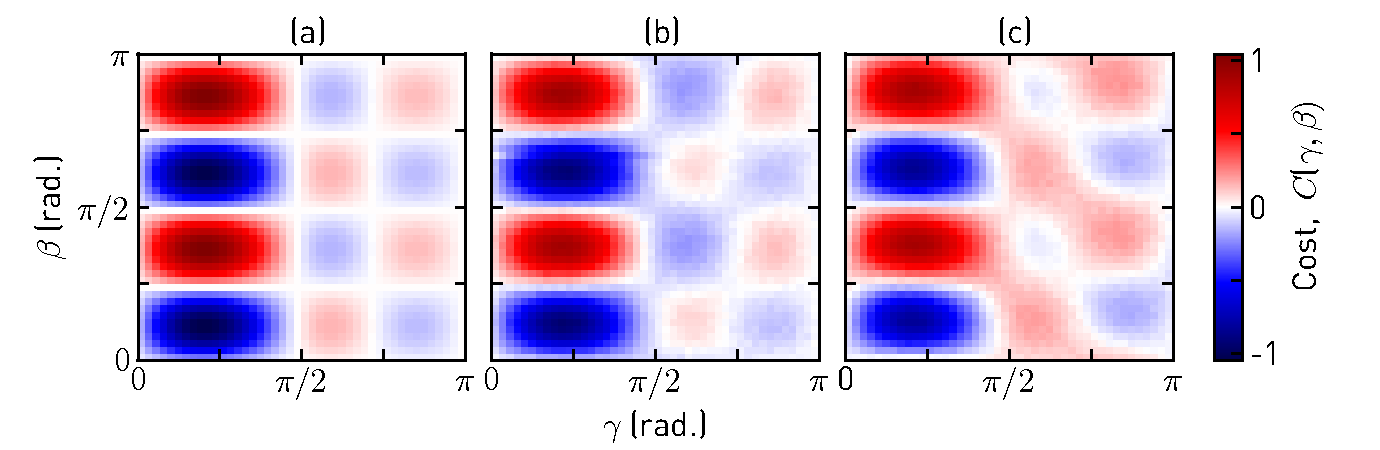
\includegraphics[width=\textwidth]{chapters/qaoa/figs/qaoa_landscapes_20200216_211657.pdf}
    \caption{Optimization landscapes for a \gls{qaoa} implementation with one layer. The two variational parameters, $\gamma$ and $\beta$ are swept over a 45x45 grid, and the cost function $\cost$ is evaluated for each parameter pair.  (a) Landscape obtained with noise-free simulation. The minimal cost function value is approximately -1.05. (b) Landscape obtained with the direct implementation of the \gls{carb}. Taken with 20000 single shot measurements per parameter pair. (c) Landscape obtained with the decomposed implementation of the \gls{carb}. Taken with 20000 single shot measurements per parameter pair. }
    \label{fig:qaoa_landscapes}
\end{figure}


\subsection{Variational parameter optimization} \label{sec:qaoa_optimization}
When no strategy is known to find the best variational angles and  $p > 1$,  classical optimizers constitute a way to navigate through the parameter space. Desirable properties to ensure rapid and consistent convergence to the optimal parameters are:
\begin{itemize}
    \item [--] \textbf{Low cost function sampling}. Each query to the quantum computer is costly in time. Therefore, optimizers minimizing the number of queries sent to the quantum computer are better suited for this task. Algorithms relying on Hessian matrix estimation are not suited, as the number of elements in the Hessian matrix grows quadratically with $p$.
    \item[--] \textbf{Robustness to noise}. Measurements from quantum computers are subject to noise. Especially when the gradient of the cost function is small, it is crucial for the algorithm to be robust to fluctuations.
    \item[--] \textbf{Capability of avoiding local minima}. At low depths, the cost functions show local minima. Algorithms capable of finding the global optimum are better suited.
\end{itemize}

We leave the task of finding the optimal classical optimizer for future work, and instead focus on comparing the performance difference of a simple optimizer between the \gls{dir} and \gls{dec}
For the sake of completeness, we briefly report on optimizers which have been applied to \gls{qaoa} in recent literature.

To find variational parameters for a single layer \gls{qaoa} implementation, Ref.~\cite{Otterbach2017UnsupervisedComputer} applied Bayesian optimization (BO)~\cite{Mockus1989GlobalApproach}, a gradient-free, global optimization method relying on Gaussian processes. Although BO performs excellently in low-dimensional parameter spaces, the number of evaluations grows exponentially with the number of parameters, rendering it impractical when $p$ is large. Ref.~\cite{Bengtsson2019QuantumProcessor} compared BO on a two-layer \gls{qaoa} implementation with the Nelder-Mead (NM) algorithm~\cite{Nelder1965AMinimization} and the covariance matrix adaptation evolution strategy (CMA-ES)~\cite{Hansen2016TheTutorial}. On their problem instance, NM has the lowest cost function sampling but is also the most sensitive to local minima due to its locality. By contrast, the CMA-ES requires more function evaluations but is stochastic and is believed to scale favorably with the number of parameters~\cite{Bengtsson2019QuantumProcessor}. For $p=2$, BO yielded a good trade-off between low cost function sampling and sensitivity to local minima. 
Ref.~\cite{Pagano2019QuantumSimulator} used problem-specific heuristics combined with a bootstrapping algorithm. Other heuristics~\cite{ZhouQuantumDevices} and deep-learning based approaches~\cite{Verdon2019LearningNetworks} have been proposed but not tested beyond simulations. Finally, the simultaneous perturbation stochastic approximation (SPSA)~\cite{Bhatnagar2013StochasticOptimization} is a promising stochastic global optimization approach not yet applied to \gls{qaoa}. The major advantage of SPSA is that it requires only two cost function evaluations per optimization step, independently of the dimensions of the parameter space.

In this work, we use the NM algorithm, due to its simplicity and low cost function sampling. To mitigate the effect of local minima, we increase the size of the initial simplex to the same order of magnitude as the distance between minima observed in Fig.~\ref{fig:qaoa_landscapes}.

 For each optimization trajectory, we initialize parameters randomly and then let the NM algorithm run 40 cost function evaluations. One function evaluation takes approximately 20-25 seconds such that an optimization trajectory takes approximately 12 minutes. In Fig.~\ref{fig:qaoa_optimization_traces}, we show the results of 15 optimization trajectories of both implementations for up to 4 \gls{qaoa} layers. Each data point of the cost function is estimated from 20000 shots. 

\begin{figure}[ht]
    \centering
    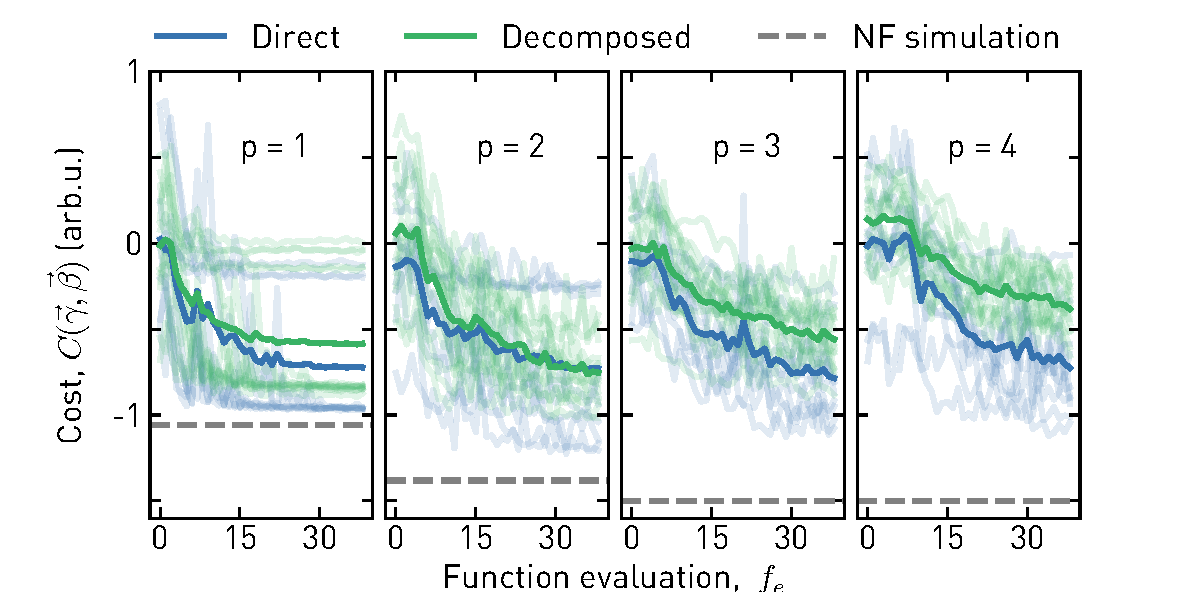
\includegraphics[width=\textwidth]{chapters/qaoa/figs/ch5_qaoa_optimization_traces_one_line_20200205_212444.pdf}
    \caption{Cost optimization trajectories for depths of $p=$ 1, 2, 3 and 4 as a function of the number of function evaluations, $f$. The variational parameters are initialized randomly and then optimized iteratively with the Nelder-Mead algorithm. Each cost value is computed from 20000 single shot measurements. The trajectories obtained with the direct (decomposed) implementation of the \gls{carb} are shown in blue (green). The faded lines correspond to the 15 individual trajectories while the darker color correspond to their average. The grey dashed line indicates the minimal achievable cost for each depth as calculated with a noise-free simulation.}
    \label{fig:qaoa_optimization_traces}
\end{figure}

The motivation for a higher number of layers becomes apparent. For $p=1$, we observe for either implementation three different convergence values of the cost function, two corresponding to the local minima and one to the global minimum, as expected from the three pairs of minima visible in Fig.~\ref{fig:qaoa_landscapes}. The local minima significantly impact the average cost at convergence. In addition, the best case performance is limited by the minimal achievable cost for $p=1$.

For $p=2$, the best trajectories of the direct implementation achieve cost below what is possible with only one layer and local minima are less apparent, although still present. 

 Three layers are required to reach the minimum cost of $-1.5$ in noise-free simulation. But adding layers does not always yield better performance. Indeed, it also results in longer gate sequences, aggravating the effect of decoherence. Moreover, additional layers increase the dimension of the parameter space, resulting in slower convergence, which is clearly visible by comparing the average trajectories for e.g.\ 1 and 4 layers. In fact, the average trajectories suggest 40 cost function evaluations do not allow the algorithm to fully converge for $p > 1$. 

For $p = 1,3,4$, the direct implementation reaches lower cost on average (for $p=2$, only its median is lower), indicating that the gate sequence length plays a major role in the performance of the algorithm. In the next section, we analyze this effect in more details. 

\subsection{Success probability as function of depth}
The previous section suggests there is an inherent trade-off: additional layers increase the performance of the algorithm in theory but also aggravate the effect of sequence-length-dependent errors in experiments. Similar conclusions were found by Alam et al.~\cite{Alam2019AnalysisQubits}. The goal of this section is to analyze how this trade-off affects the two implementations of the \gls{qaoa}.

Note that the (approximate) solution of a problem found with \gls{qaoa} is the measured bit-string after optimization of the variational parameters. Therefore, a crucial metric to assess the performance is the success probability, $P_s$ (see Section~\ref{sec:qaoa_success_prob}) and not the cost function used for classical optimization of the variational parameters. 

To investigate the effect of the depth $p$ on $P_s$ accurately, we seek to mitigate the influence of the classical optimizer on $P_s$ (namely, the influence of local minima and the convergence speed, which are expected to be equal for both implementations). To this extend, we provide an educated initial guess for the variational parameters. Namely, we first find optimal parameters for each depth in a noise-free simulation and provide these theoretically optimal parameters for the initialization of the quantum computer. Under the assumption of equal depolarization, bit-flip and dephasing channels for all qubits, the optimal variational parameters remain nearly the same in a noise-free and noisy environment, according to a recent theoretical investigation~\cite{Xue2019EffectsAlgorithm}. Because coherence times and coherent errors are not exactly equal for all qubits on our device, we additionally optimize locally with up to 20 function evaluations on the quantum computer. 

We show the result of the above-mentioned protocol in Fig.~\ref{fig:qaoa_sequence_lengths}. The success probability for various depths is plotted versus sequence length, $L$, to facilitate the comparison of sequences of similar lengths independently of the implementation. The dashed lines correspond to the expected success probability in a noise-free environment. 

\begin{figure}[ht]
    \centering
    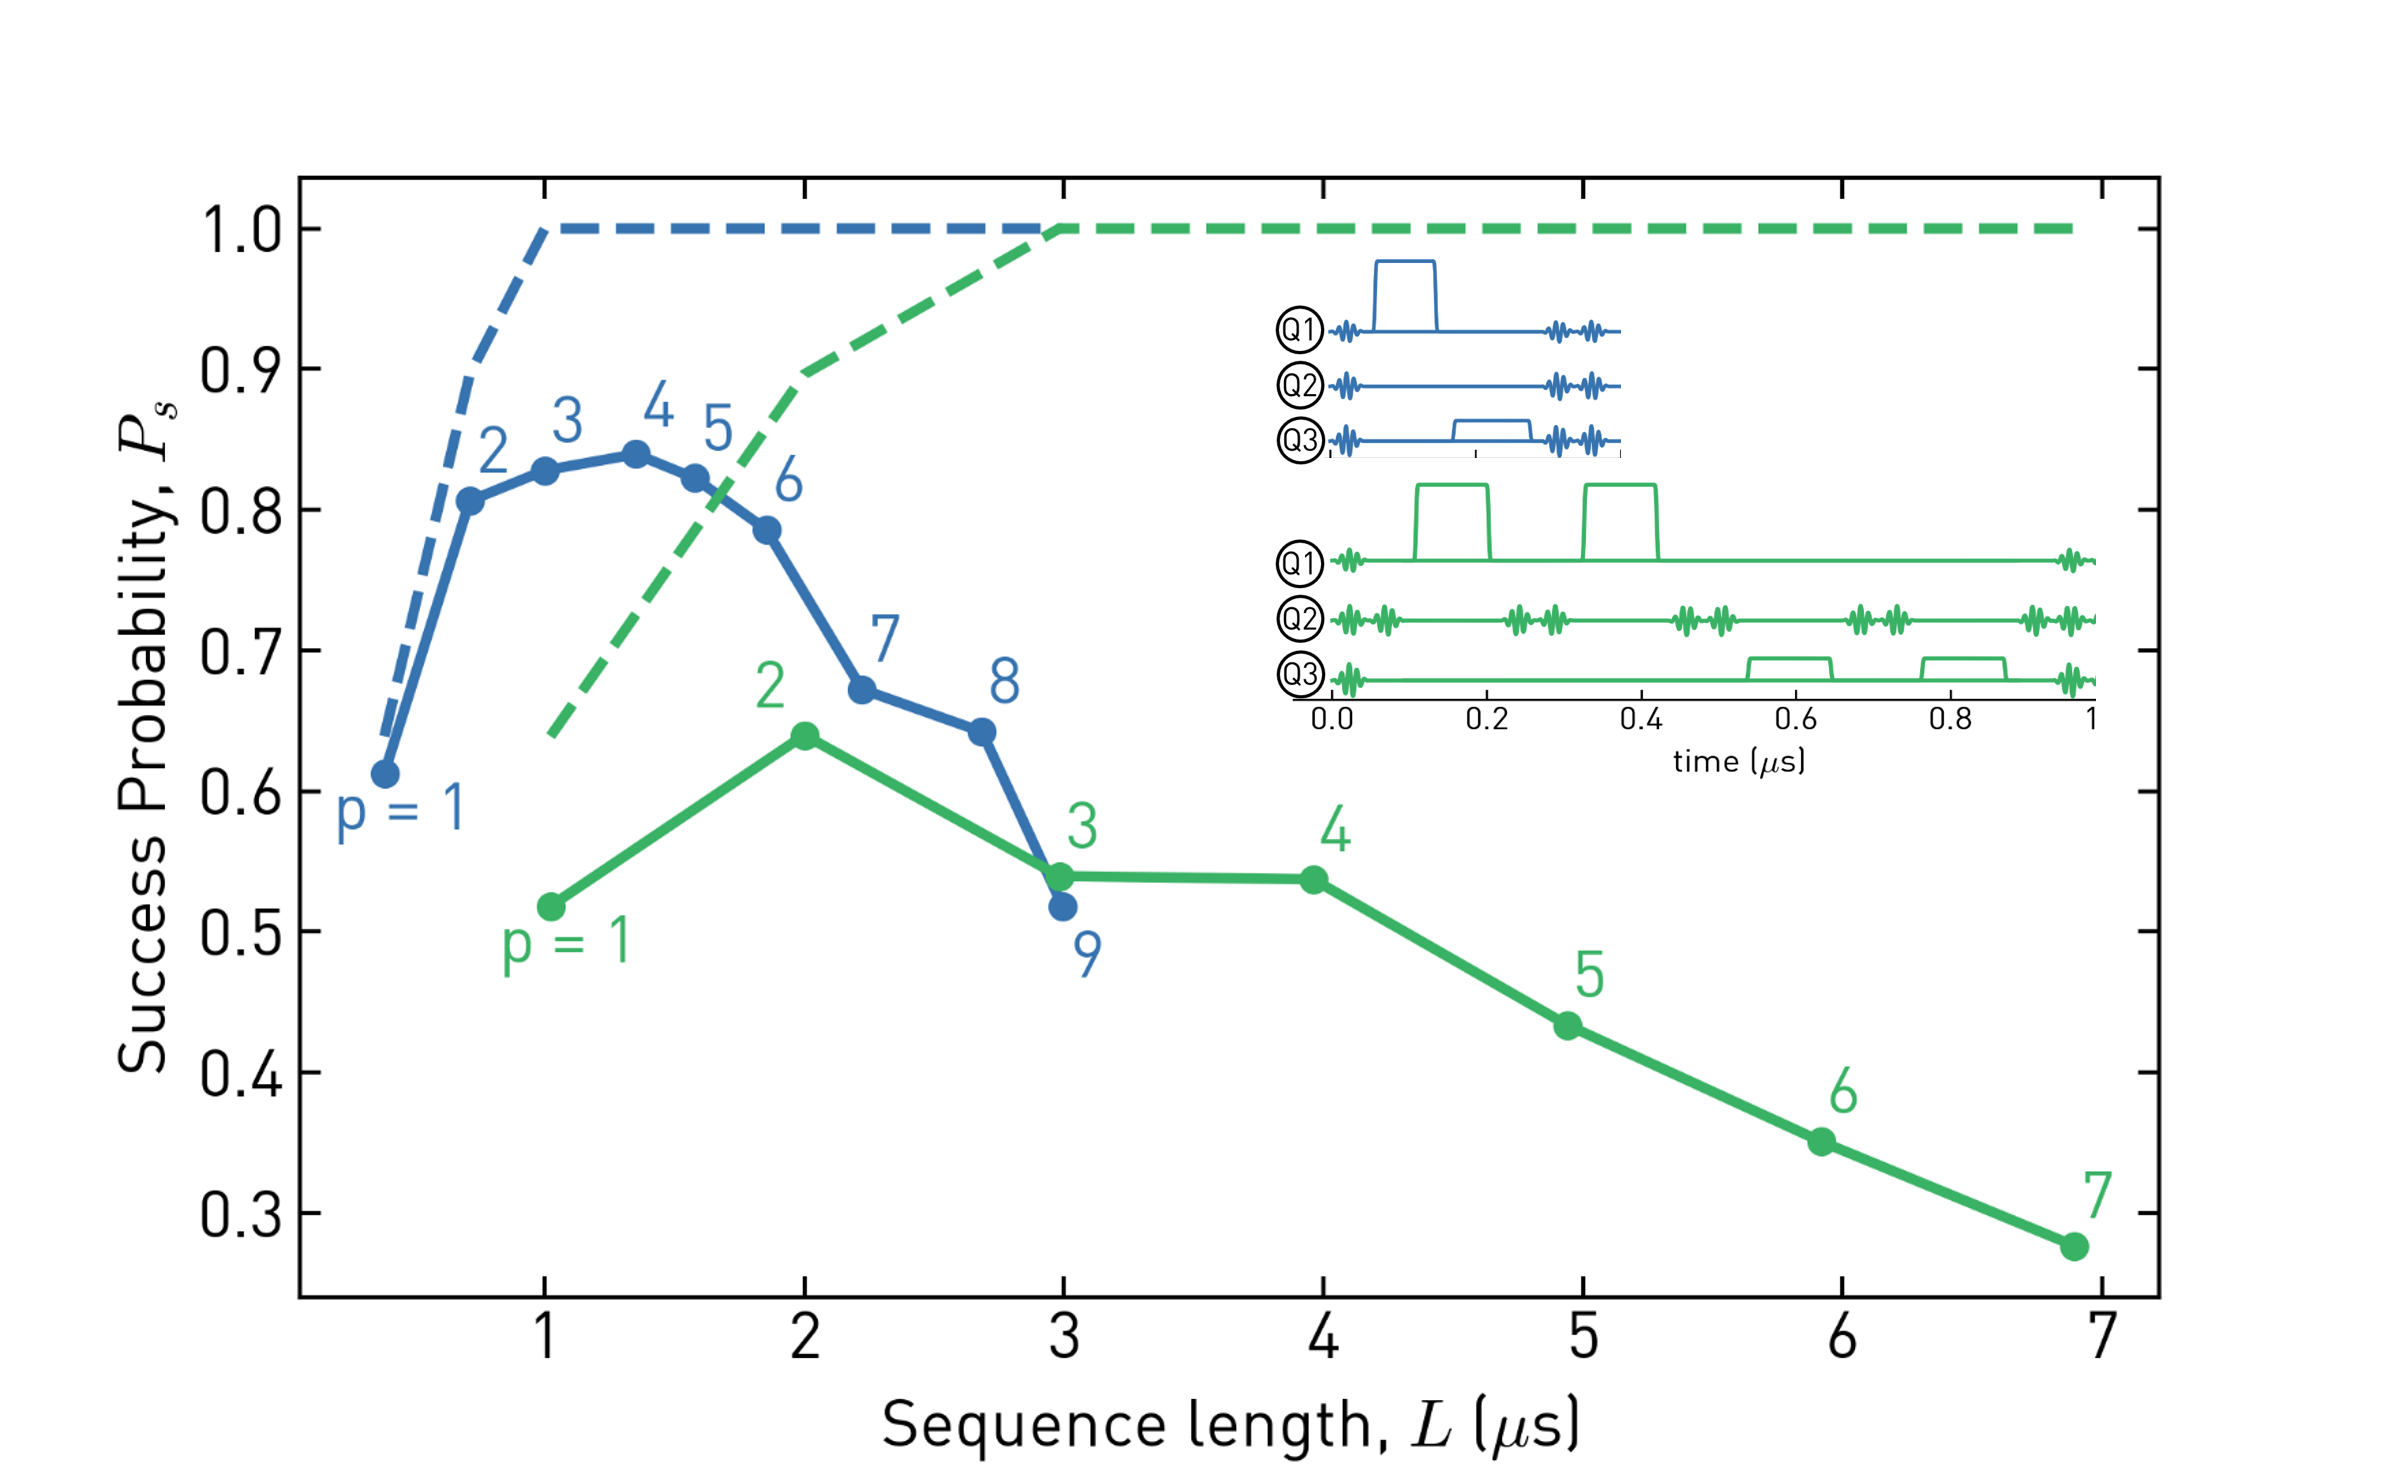
\includegraphics[width=\textwidth]{chapters/qaoa/figs/ch5_qaoa_sequence_lengths_v1_withinset_20200202_120000.png}
    \caption{Success probability as a function of sequence length for the direct (blue) and decomposed (green) implementations of the \gls{carb}. The dashed line of corresponding color indicates the success probability as calculated by a noise-free simulation. The depth is annotated next to the data points. For each depth, the quantum computer is initialized with variational parameters obtained from the noise-free simulation. The corresponding pulse schemes for one layer are shown in the inset.}
    \label{fig:qaoa_sequence_lengths}
\end{figure}

The \gls{dir} exhibits a clear advantage: in about $1\,\mu\text{s}$, it is able to execute a 3 layers of \gls{qaoa} while the decomposed implementation only carries out one. For a fixed depth, it consequently suffers less from errors scaling with the sequence length. 

The difference in sequence length arises from the combination of two factors (see inset of Fig.~\ref{fig:qaoa_sequence_lengths} for the full pulse sequence for $p=1$):
\begin{enumerate}
    \item The decomposition of each \gls{carb} requires two individual \gls{cz} and 4 single-qubit gates. 
    \item The \gls{carb} is shorter than the \gls{cz} for any conditional phase different from $\pi$.
\end{enumerate}
Moreover, the number of \glspl{carb} grows with $\mathcal{O}(m\cdot p)$, where $m$ indicates the number of two-qubit terms in \costh{} which cannot be executed simultaneously. Therefore, the total decomposed sequence length rapidly becomes much longer. 

As mentioned in Section~\ref{sec:qaoa_optimization}, noise-free simulations require in the ideal case 3 layers to reach $P_s \approx 1$, which for the \gls{dec} is realized with $L \approx 3\, \mu\text{s}$. For that sequence length, the \gls{dir} can implement up to nine layers. However, in Fig.~\ref{fig:qaoa_sequence_lengths} we observe that both implementations show similar performance for $L \approx 3\, \mu\text{s}$, which directly indicates that performance is limited by sequence length rather than the number of layers.
In particular, in our case we expect both conditional phase errors due to residual $ZZ$-coupling and decoherence to have a major impact which scales with sequence length.

To gain further insights into the performance of the algorithm, we present in Fig.~\ref{fig:qaoa_state_histogram} the full distribution of measured bit strings for each of the first 4 points ($p=1,2,3,4$ for each implementation) of Fig.~\ref{fig:qaoa_sequence_lengths}. The colored dots in the right panel indicate the respective success probabilities, i.e.\ the sum of the probabilities for states $\ket{010}$ and $\ket{101}$ (colored bars). The right panel also shows the success probability distribution (faded filling) of the optimization trajectories discussed in Section~\ref{sec:qaoa_optimization}. If the trajectories constitute a representative sampling of the parameter space, the dot should lie at the right edge of the distribution. A data point outside the distribution suggests the trajectories did not converge to the lowest possible value, or did not find the global cost optimum, for instance because of a local minimum. Conversely, a data point inside the distribution suggests the initialization from theoretically optimal variational parameters is not perfect, or fluctuating performance compared to when the trajectories were recorded.

\begin{figure}[ht]
    \centering
    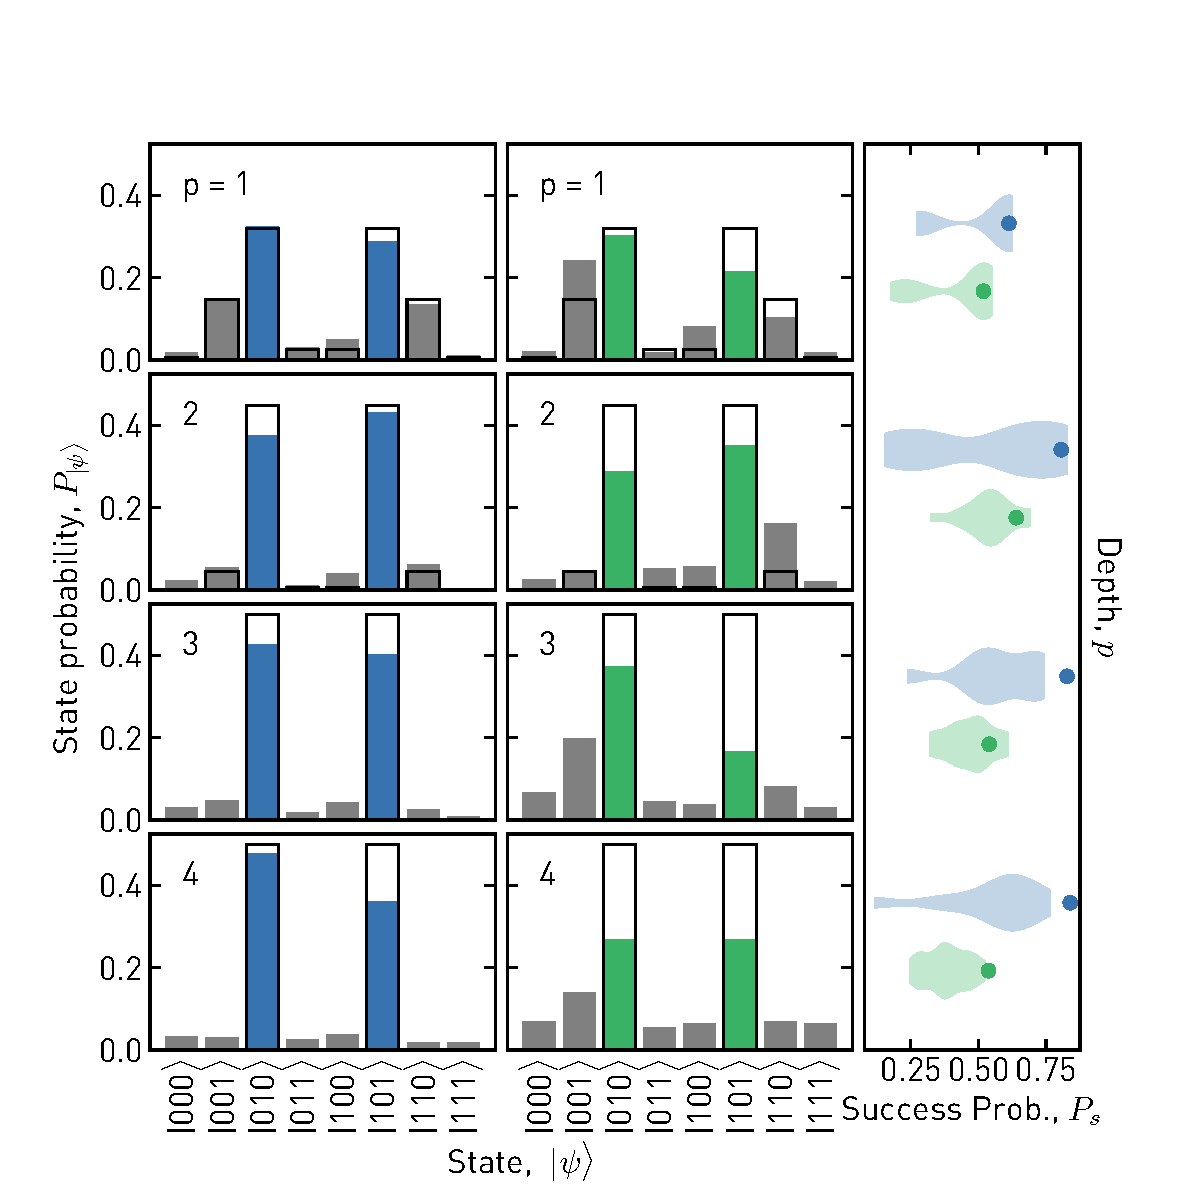
\includegraphics[width=\textwidth]{chapters/qaoa/figs/ch5_qaoa_state_histograms_20200202_134816.pdf}
    \caption{Distribution of measured states for the \gls{dir} (left) and \gls{dec} (middle) for $p=1,2,3,4$. The black wire-frame corresponds to the noise-free simulation distribution of states and is equal for both implementations, at fixed depth. For each distribution, the highlighted bars correspond to solutions of the exact cover problem. Their sum amounts to $P_s$, shown on the right panel with dots of corresponding color (also corresponding to the first 4 dots for each implementation in Fig.~\ref{fig:qaoa_sequence_lengths}). The faded distributions in the right panel correspond to the success probability of the optimization trajectories presented in Fig.~\ref{fig:qaoa_optimization_traces}.}
    \label{fig:qaoa_state_histogram}
\end{figure}

In the state distributions, the most likely states are $\ket{101}$ and $\ket{010}$, corresponding to the desired sets $\mathcal{L}_1' = \{A,C\}$ and $\mathcal{L}_2' = \{B\}$ defined in Section~\ref{sec:qaoa_exact_cover}. The \gls{dir} is in excellent agreement with the noise-free simulation (black wire-frame) for all depths, and achieves a success probability of $0.84$ at $p=4$\footnote{In principle three layers are sufficient to reach $P_s \approx 1$ and additional layers are expected to suffer from additional errors, thereby showing a decrease in success probability. However, the classical optimizer also allows to compensate for some errors and more parameters provide additional degree of freedom to correct for errors.}. By contrast, the \gls{dec} consistently shows more deviations from the simulation and achieves a maximal success probability of $0.64$\footnote{Note that one of the optimization trajectory starting from random initialization reaches a success probability of $0.69$ at $p=2$. We attribute this difference to fluctuations in coherence times and gate performance} at $p=2$. 

We conclude that the trade-off of additional layers affects the two implementations of the \gls{carb} differently. The success probability of the \gls{dir} increases for up to four layers before being decreasing due to decoherence and accumulated phase errors, thereby achieving a success probability of 0.84. On the other hand, the \gls{dec} can only execute two layers before being affected by sequence length dependent errors, which is not sufficient to reach the regime where the success probability is near unity even in the noise-free simulation.

\section{Conclusion}
\glsreset{qaoa}

In this chapter, we have found approximate solutions for a three-qubit exact cover problem instance using the \gls{qaoa}. The problem instance requires at least three layers of the \gls{qaoa} in the ideal case to reach a success probability approaching unity, as determined by noise-free simulations. To the best of our knowledge, this constitutes the deepest problem considered in the experimental \gls{qaoa} literature. 

We have shown that for this problem instance, the direct implementation of two-qubit interaction terms in each layer of the \gls{qaoa} reduces the two-qubit gate-count by 50\% and the executed gate-sequence length by a factor of $\sim 3$ compared to a decomposition into 2 \glspl{cz} and 4 single-qubit gates. Exploiting this advantage, we demonstrate a success probability of $0.84$ using 4 layers of \gls{qaoa}. In comparison, the decomposed implementation reached a maximal success probability of $0.64$ with 2 layers as it is more affected by decoherence and residual $ZZ$-coupling. Experimental observations also strongly suggest that decoherence and residual $ZZ$-coupling are the dominant error sources in both implementations.

The sequence length reduction factor enabled by \glspl{carb} scales approximately linearly with the number of two-qubit terms in the cost Hamiltonian which cannot be executed simultaneously. Typically, the number of two-qubit terms grows with the number of qubits in the problem instance. We therefore expect a considerable performance gain on near-term quantum processors with 10-1000 qubits, as a linear reduction in sequence length avoids exponentially increasing incoherent errors.  In summary, this work provides tangible evidence that \glspl{carb} open the door to solving more complex problem instances on quantum computers for as long as the algorithm's performance are limited by decoherence. 


\chapter{Conclusion}
\glsresetall{}

% Large-scale, fault-tolerant quantum computing has the potential to impact numerous fields such as chemistry, medical research, material science, information security and logistics. However, building large-scale and noise-free quantum computers is a substantial challenge. Consequently, near-term quantum computers will only have a limited number of quantum bits (qubits) and a limited computing time during which operations are executed reliably.

% \Glspl{vqa} are good candidates to take advantage of the quantum hardware in the near-term because they offset part of the computation to classical computers and are intrinsically more robust to noise mostly because they seek approximate solutions. The available computation time remains nevertheless limited by time-dependent errors such as decoherence and residual $ZZ$-coupling.

In  this  thesis,  we  demonstrated  a  way  to  enhance  the  performance  of \glspl{vqa} by reducing the  sequence length  required  to implement their circuit on quantum hardware. In particular, we enlarged the gate-set available on the quantum computer with a \gls{carb}, which enables us to avoid decomposition of higher order operations into multiple gates. 

The \gls{carb} is a generalized version of the controlled $\pi$-phase two-qubit gate (CZ gate). It is able to reach any phase on the \oo{} state between 0 and $2\pi$. Our implementation achieves an average process fidelity of 97.7\%, whereby the remaining errors are dominated by decoherence and effects of thermal population. The average leakage per gate amounts to 1.4\%, which is slightly lower than the leakage we obtain for a CZ gate implemented on the same physical qubits.

We demonstrated the advantage of \gls{carb} on a three qubit exact cover problem instance which we solved using the \gls{qaoa}, a \gls{vqa} that finds approximate solutions to combinatorial problems.  The instance we considered is the first experimental implementation requiring three QAOA layers to be solved with high success probability. 

We obtain a 50\% two-qubit gate count reduction and a gate sequence length reduction factor of 3 using the direct implementation of the \gls{carb} compared to a decomposition into \glspl{cz} and single qubit gates. Consequently, we achieve a higher success probability with the direct implementation (0.84 versus 0.64) because it executes more layers for a fixed sequence length. 

We foresee an even more pronounced advantage for larger-scale experiments because the number of layers required to solve problems typically scales with the number of qubits involved in the experiment. Therefore, for as long as quantum devices are limited by decoherence, \glspl{carb} will open the door to solving more complex problem instances with \gls{vqa}.

\appendix

\chapter{Setup}
\label{app:setup}

You can defer lengthy calculations that would otherwise only interrupt
the flow of your thesis to an appendix.


\backmatter

\bibliographystyle{plain}
\bibliography{references_mendeley}

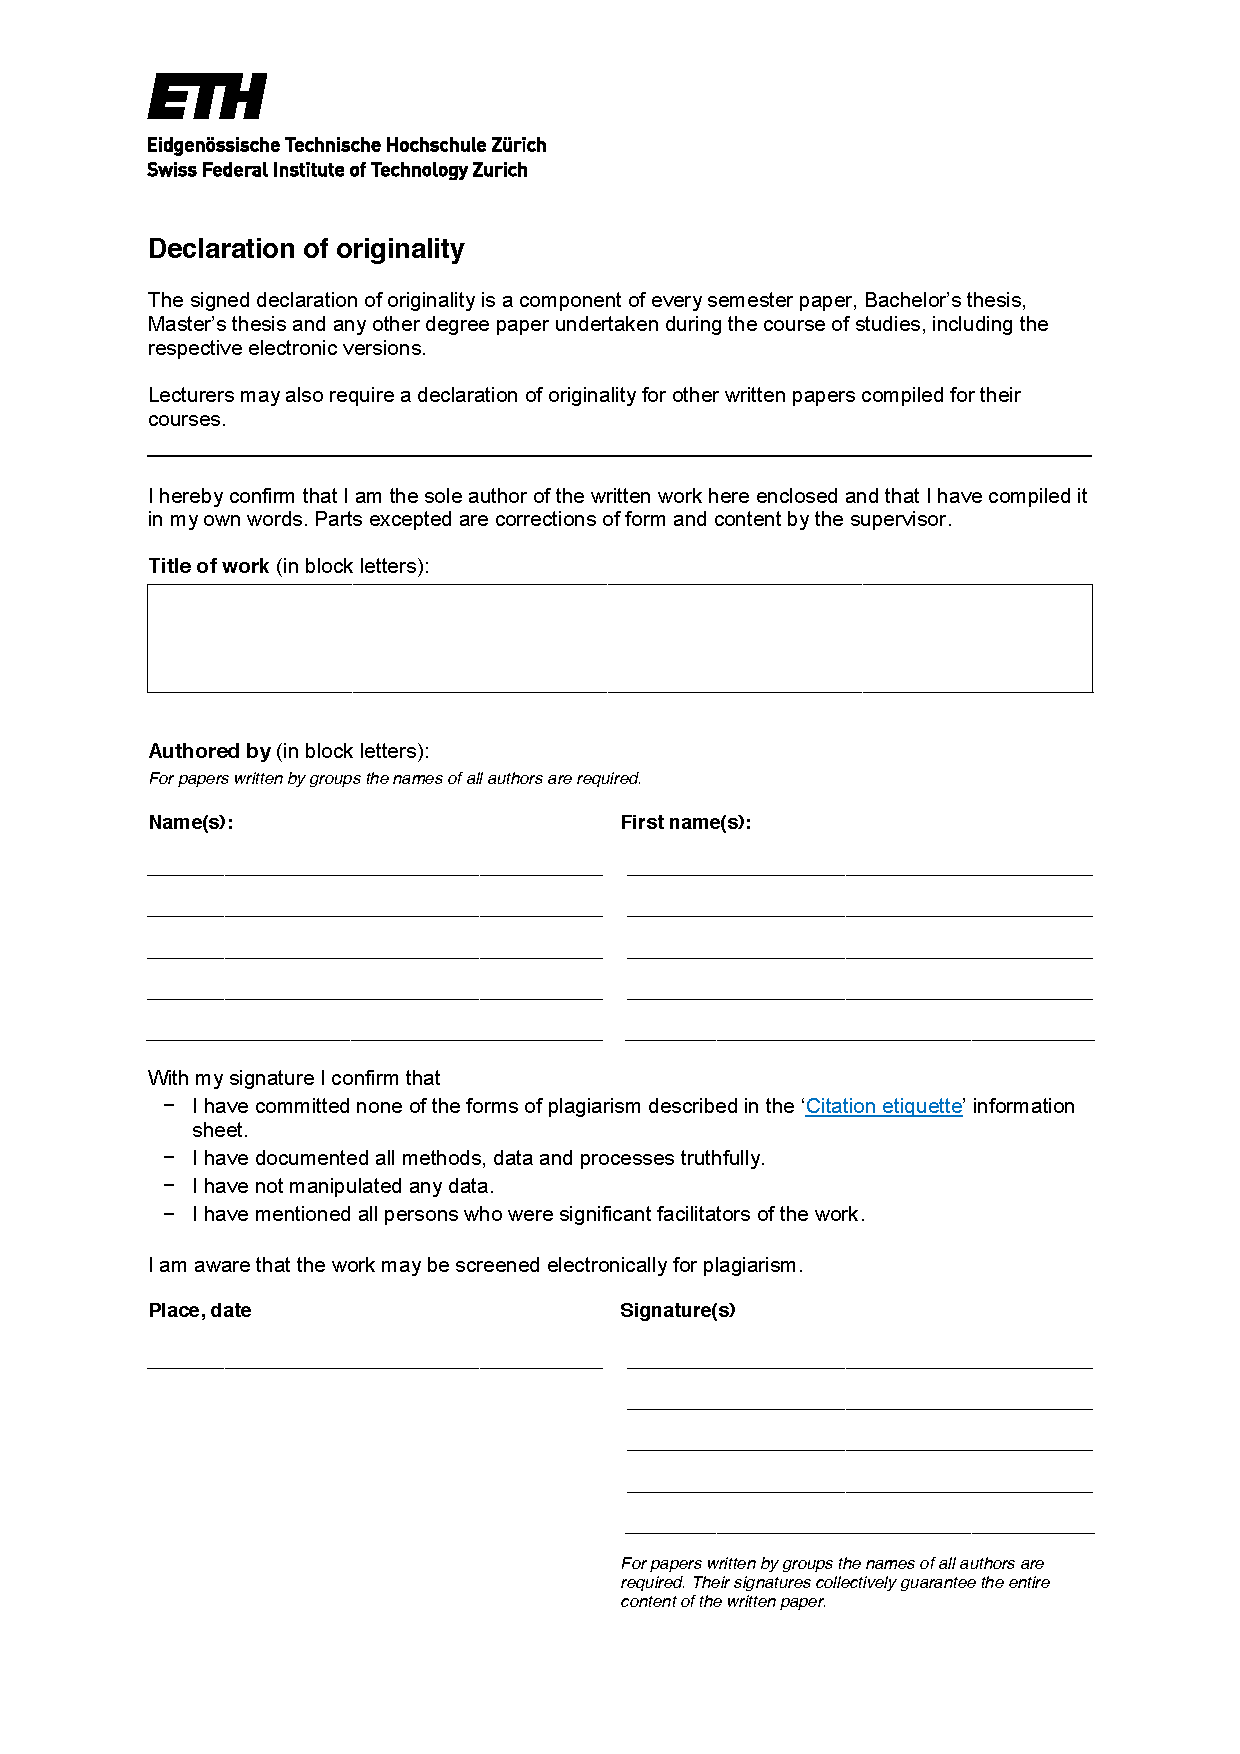
\includepdf[pages={-}]{declaration-originality.pdf}

\end{document}
